\section{Entities}\label{sec:01}
In order to access the Bakery System, You should be registered as a User therein. 
After the registration a User can log in to the system using their username and password.

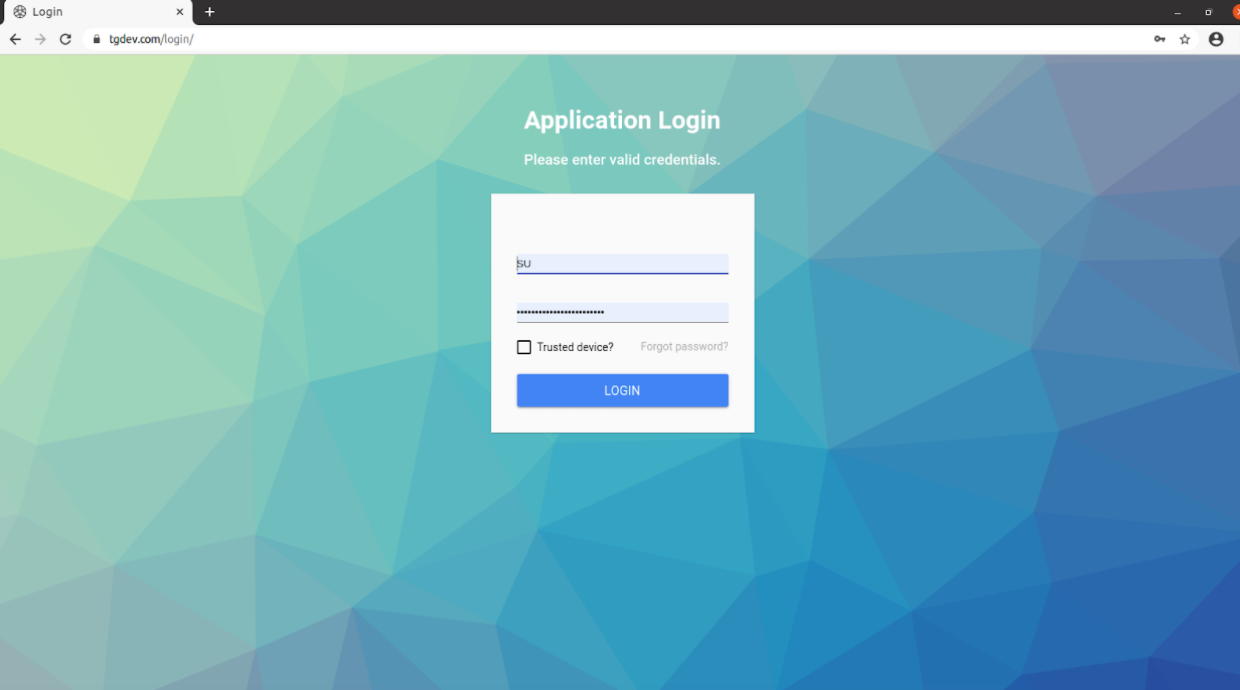
\includegraphics[width=\textwidth]{sections/01-chapter/images/login.png}

The System consists of multiple entities - key players in the system, which are used.

The System consists of 3 sections:

- User and Personnel 

- Logistics

- Production

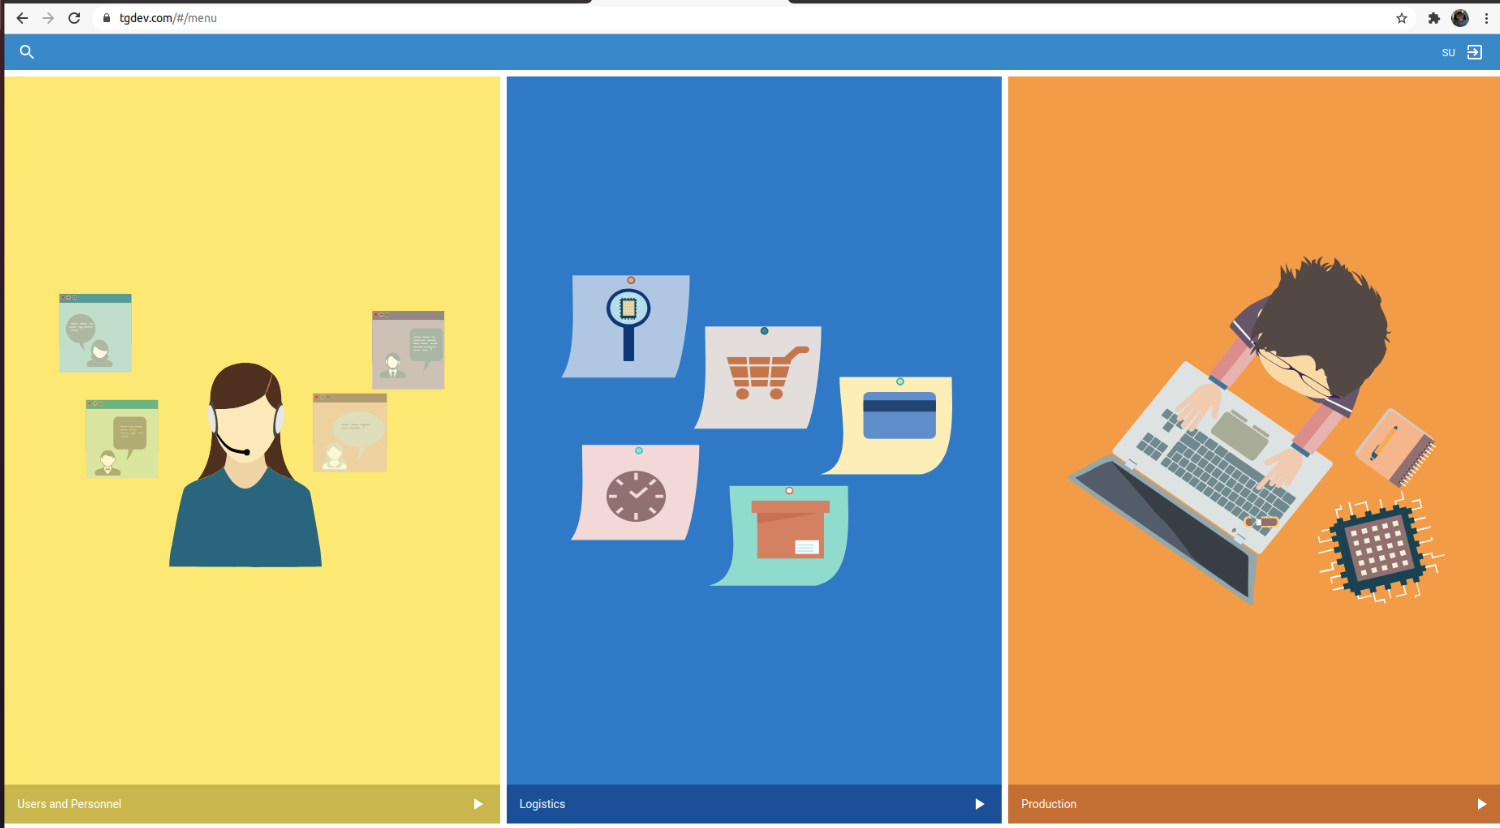
\includegraphics[width=\textwidth]{sections/01-chapter/images/main.png}


You can review them by clicking on the corresponding part of the screen.

\section{User and Personnel}

User and Personnel section includes all of the information regarding roles of persons and their employment. The roles are:

- Person 

- Manager

- Carrier

- Employment

You can review them by clicking:

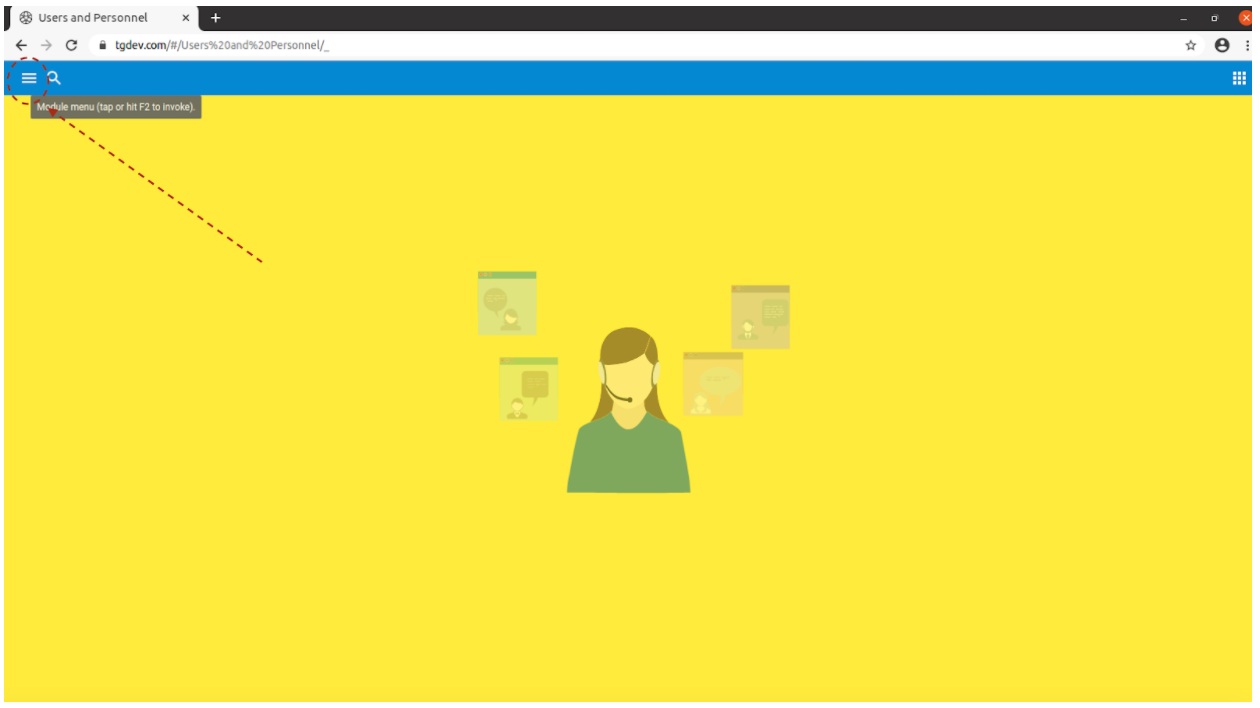
\includegraphics[width=\textwidth]{sections/01-chapter/images/review1.png}



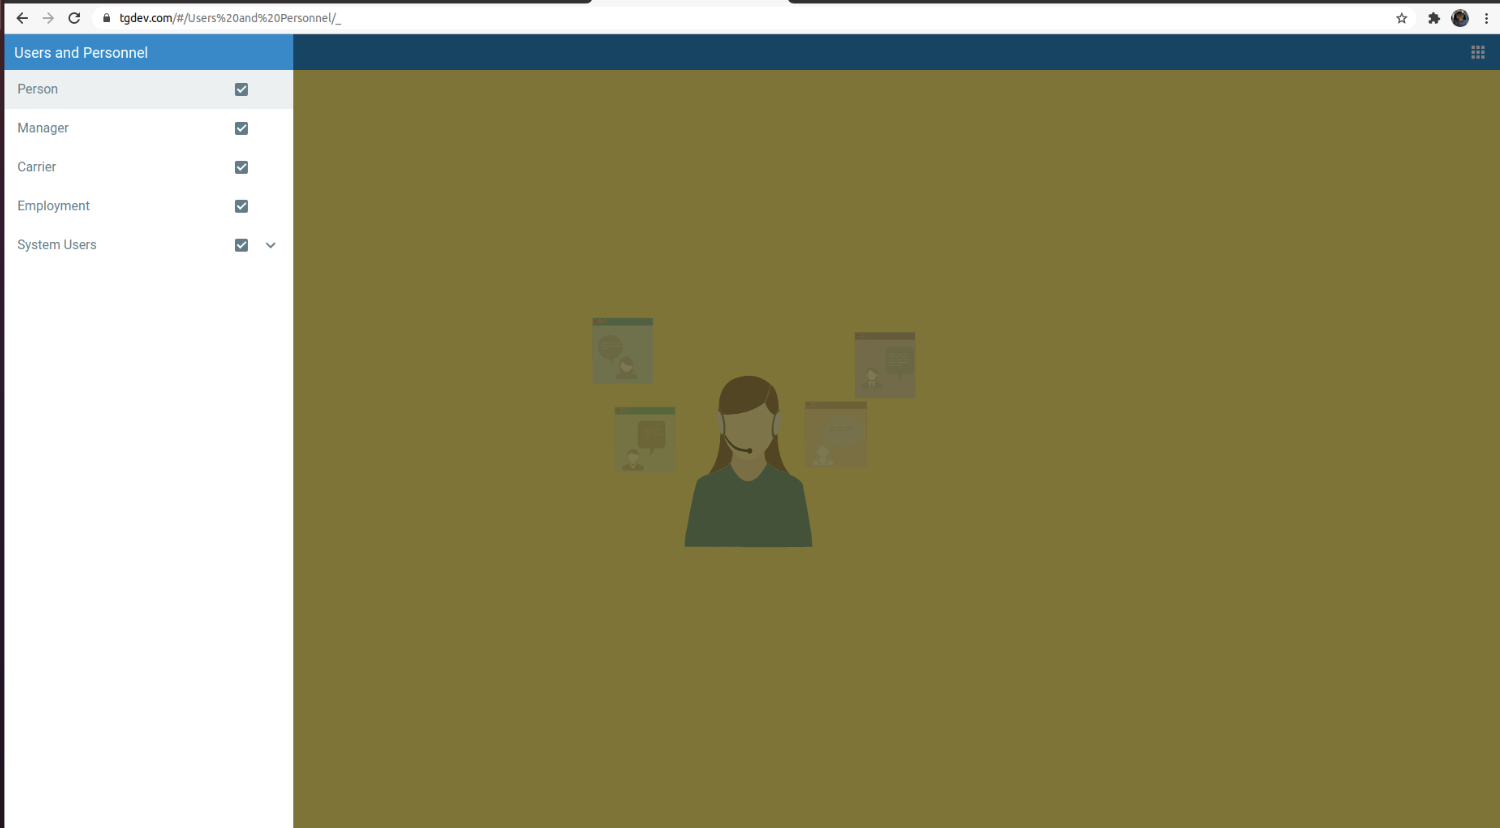
\includegraphics[width=\textwidth]{sections/01-chapter/images/personnel.png}



Depending on the role that a user has in the system, they can either have the ability to register and edit some entities or not. 

\subsection{Person}
A person represents an entity that is any person (they can be either one of the workers in a bakery or just a person).

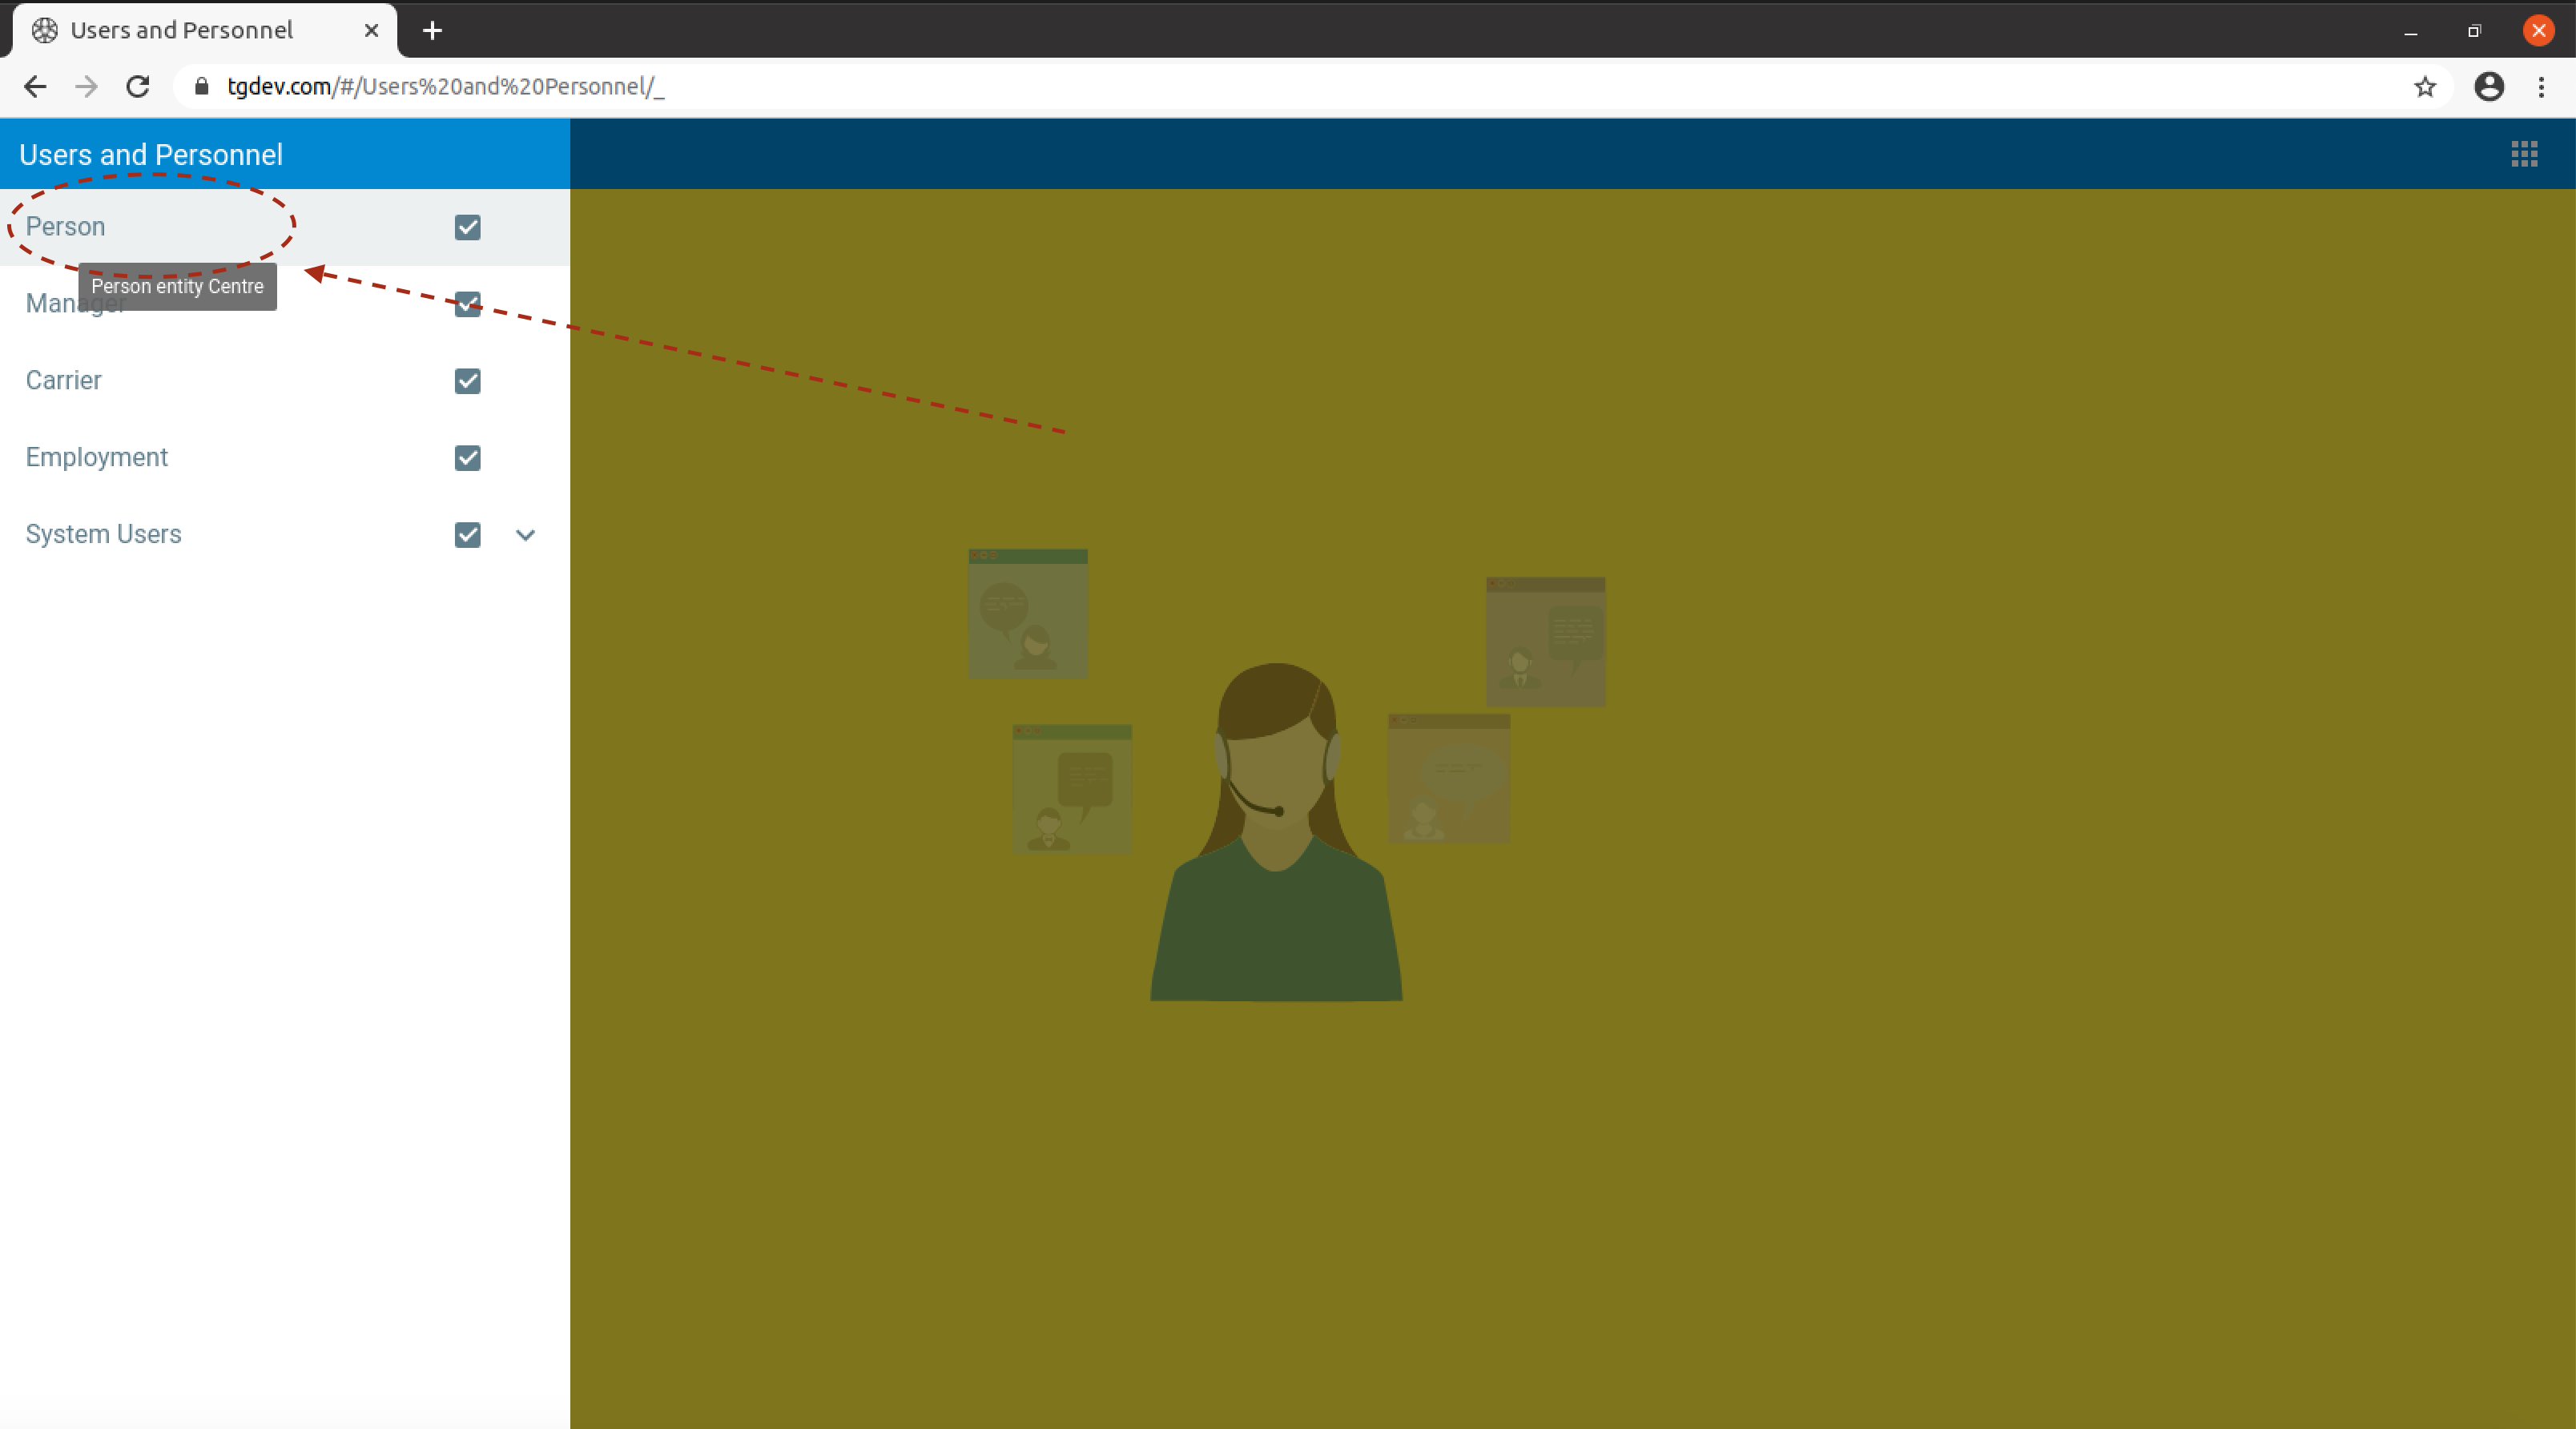
\includegraphics[width=\textwidth]{sections/01-chapter/images/person11.png}

\textbf{Creation of a new Person}

In order to create a new Person Entity you can click on: 

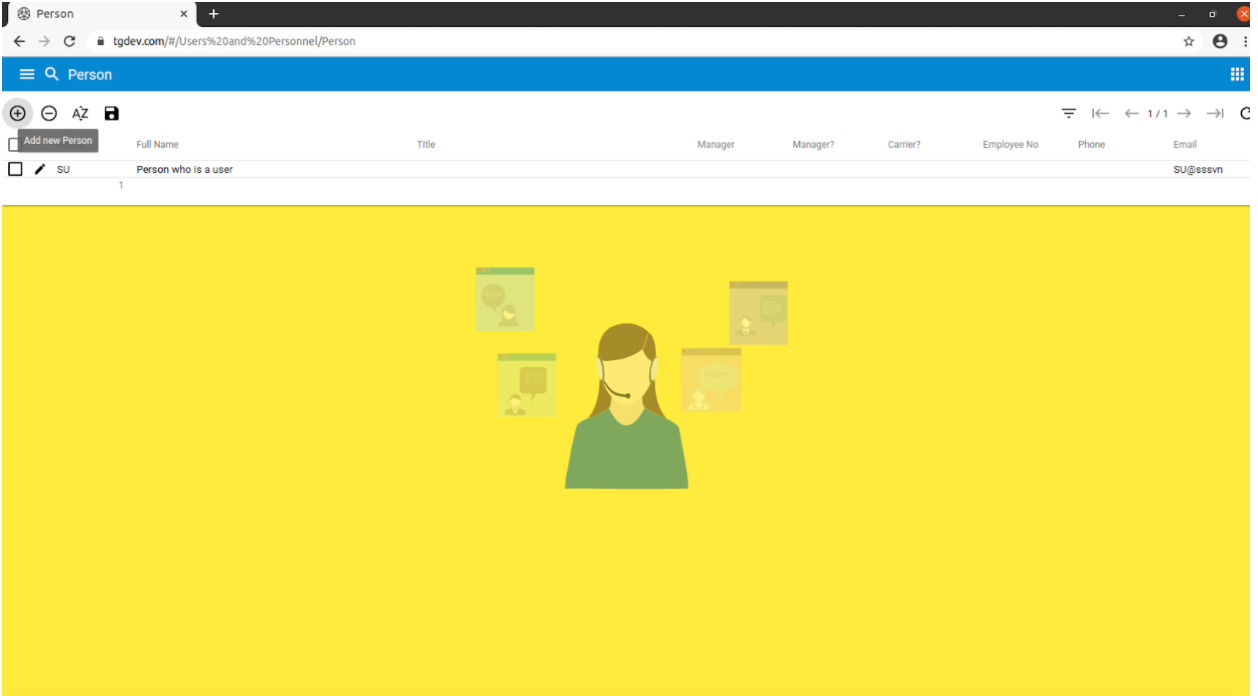
\includegraphics[width=\textwidth]{sections/01-chapter/images/person2.png}

And you need to  fill in the important fields such as:

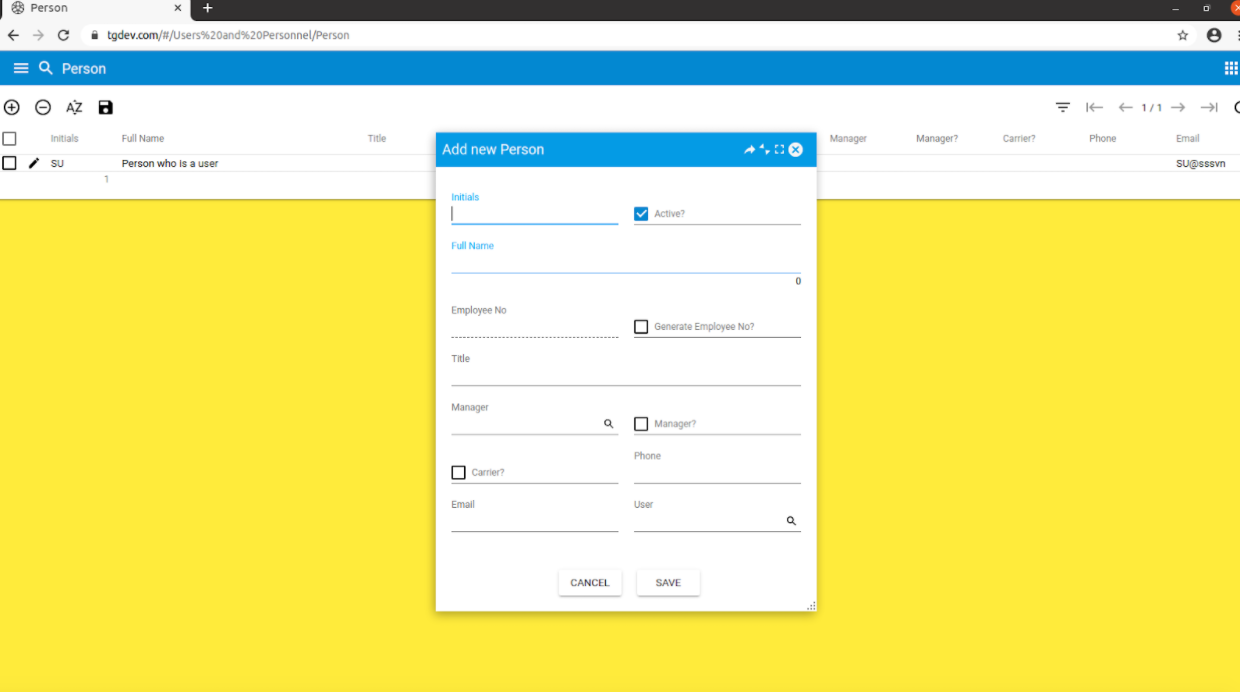
\includegraphics[width=\textwidth]{sections/01-chapter/images/person3.png}

- Initials →  required, string, spaces are not allowed in the initials

- Active → required, the indicator of an active participant in the system. The environment cannot interact with inactive Person.

- Title →  optional, person’s position.

- Employee Number → optional, the indicator number of the employee, can be generated automatically, if specified in the checkbox to the right, then position must be specified (cannot be left empty) as well. 

- Phone number → optional String, phone number of a Person

- Email →  optional, String, email

- aManager →  optional, Manager of this employee, this field is required if Employee Number is specified. In other words, every Person who has an employee number must also have a manager.

- Manager? →  optional checkbox, indicates whether this employee is in the manager role

- Carrier? → optional checkbox, indicator of whether this Person is a carrier

- User → optional, a system user associated with this Person

You can search for a Person using the following properties: 

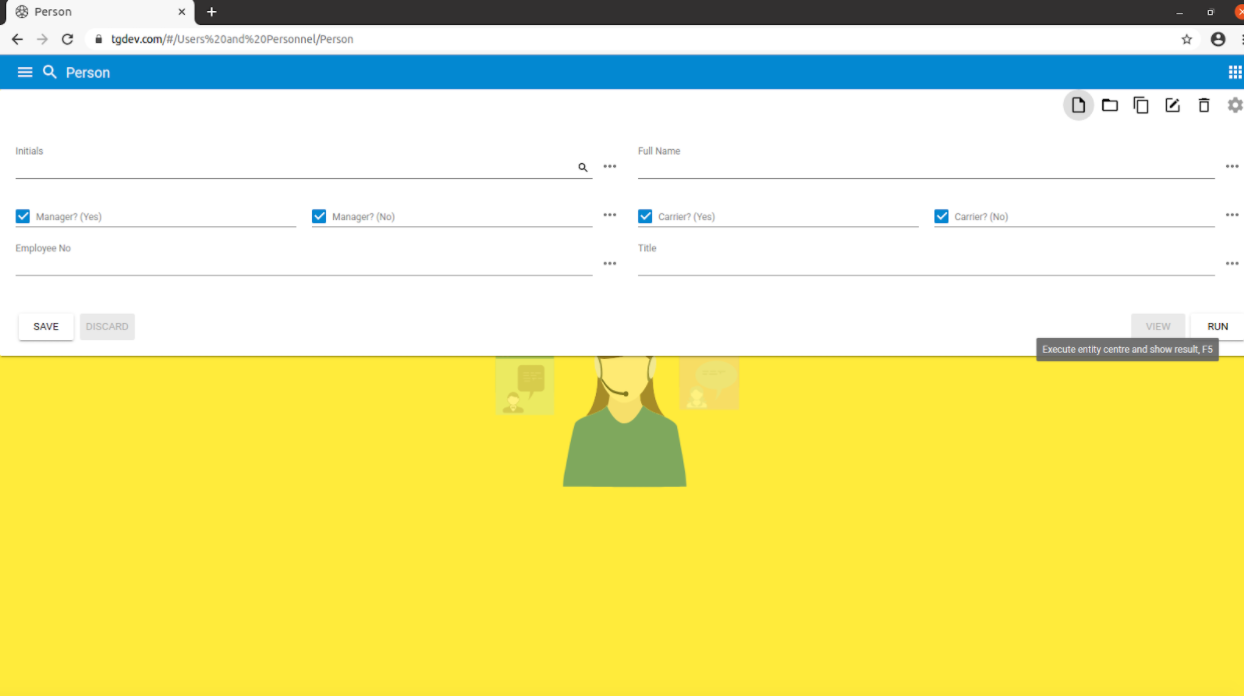
\includegraphics[width=\textwidth]{sections/01-chapter/images/person4.png}

\subsection{Manager}
A manager represents an entity that is technically a person assigned to the manager`s role.

\textbf{Creation of a new Manager}

One cannot add a Manager to the database straightforwardly. 
A manager can be added only during registration of a Person by clicking on Manager? checkbox which indicates that a person is in the manager role now.
An important thing here: Employee number must be specified in order to assign person as a Manager.

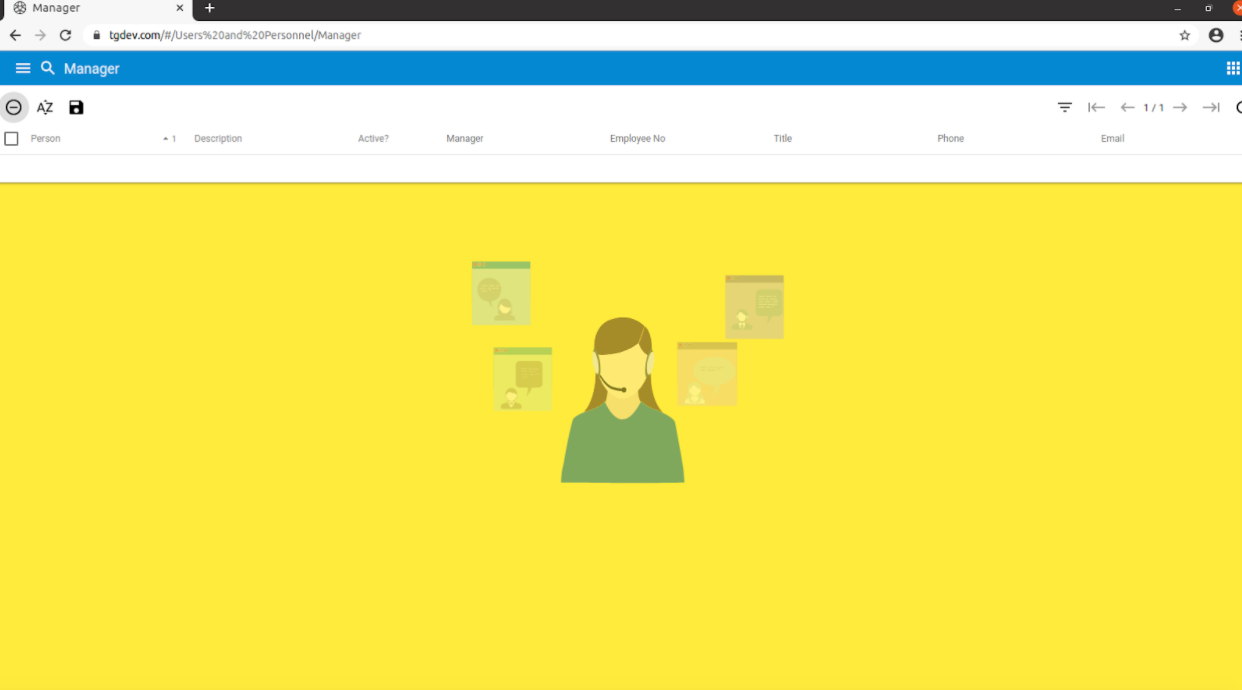
\includegraphics[width=\textwidth]{sections/01-chapter/images/manager1.png}

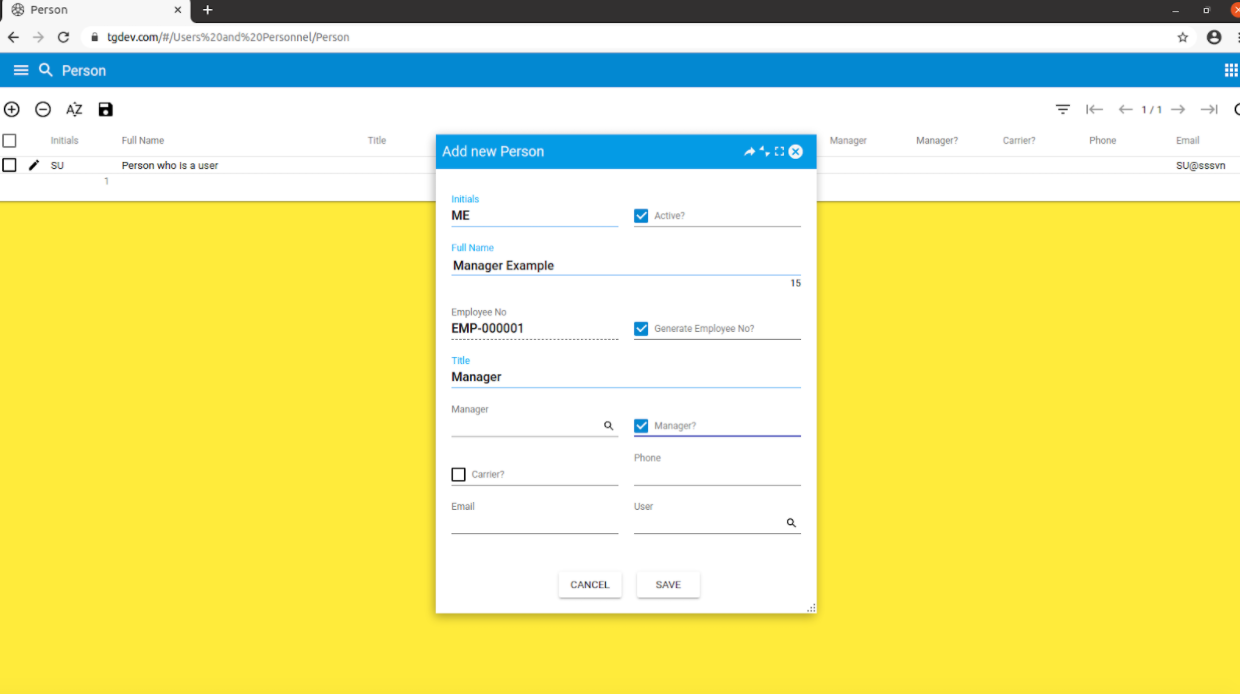
\includegraphics[width=\textwidth]{sections/01-chapter/images/manager2.png}


The required fields for a manager are:

- Employee No → the indicator number of the employee, can be generated automatically, if specified in the checkbox to the right.

- Title → the role, position of an Employee in the Bakery system

In addition, the standard fields are required:

- Initials

- Active? checkbox - which indicates whether the system can further use can interact with the Manager/ The indicator of an active participant in the system. The environment cannot interact with inactive Person.

- Full Name

The rest of the fields are optional and the same as described in Person.

Some of the constraints in this part: Manager cannot manage themselves and Manager cannot manage a non-employee.

\subsection{Carrier}

A carrier cannot be added to the table of carriers straightforwardly. It can only be added to the table by clicking the Carrier? checkbox during the registration of a Person:

A Carrier should have its EmployeeNo, Title, and a manager assigned to it. 

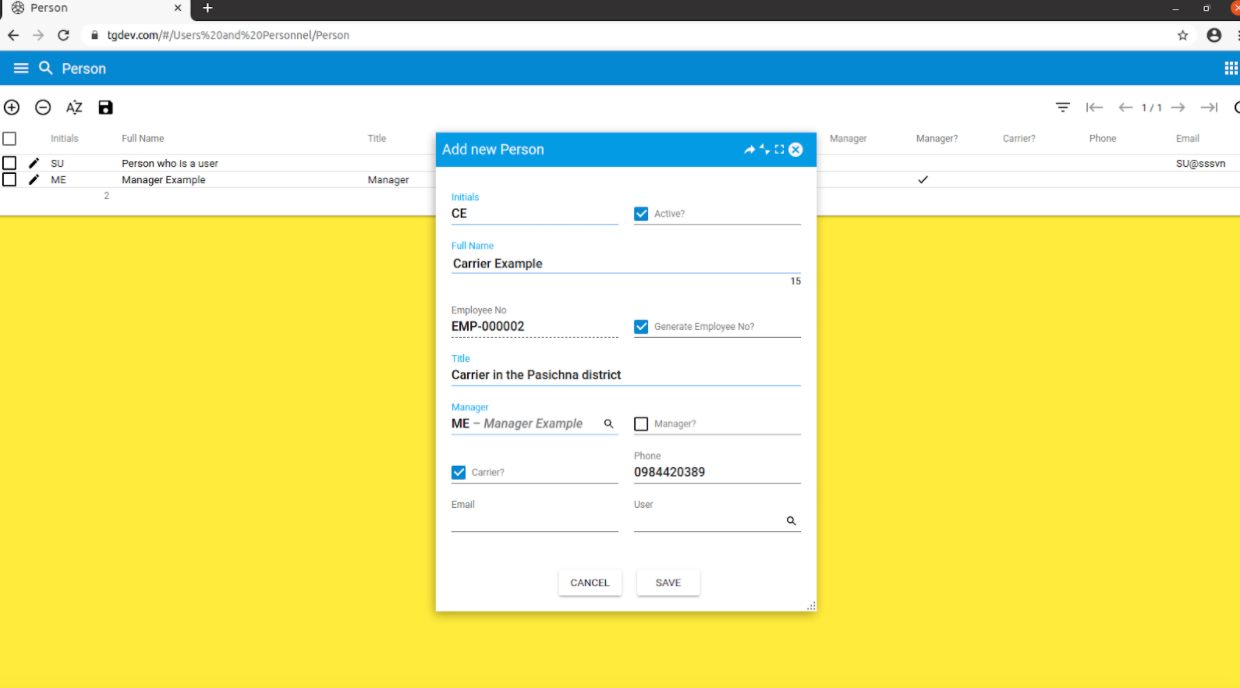
\includegraphics[width=\textwidth]{sections/01-chapter/images/carrier1.png}

The required for a Carrier fields are: 

The required fields for a manager are:

- Employee No → the indicator number of the employee, can be generated automatically, if specified in the checkbox to the right.

- Manager → The Manager of a Carrier

In addition, the standard fields are required:

- Initials

- Active? checkbox - which indicates whether the system can further use can interact with the Manager/ The indicator of an active participant in the system. The environment cannot interact with inactive Person.

- Full Name

The rest of the fields are optional and the same as described in Person.

\subsection{Employment}

Employment module represents a concept of employment in the bakery and stores all the important information about this process.

In order to look for existing employment, one should choose Employment entity.

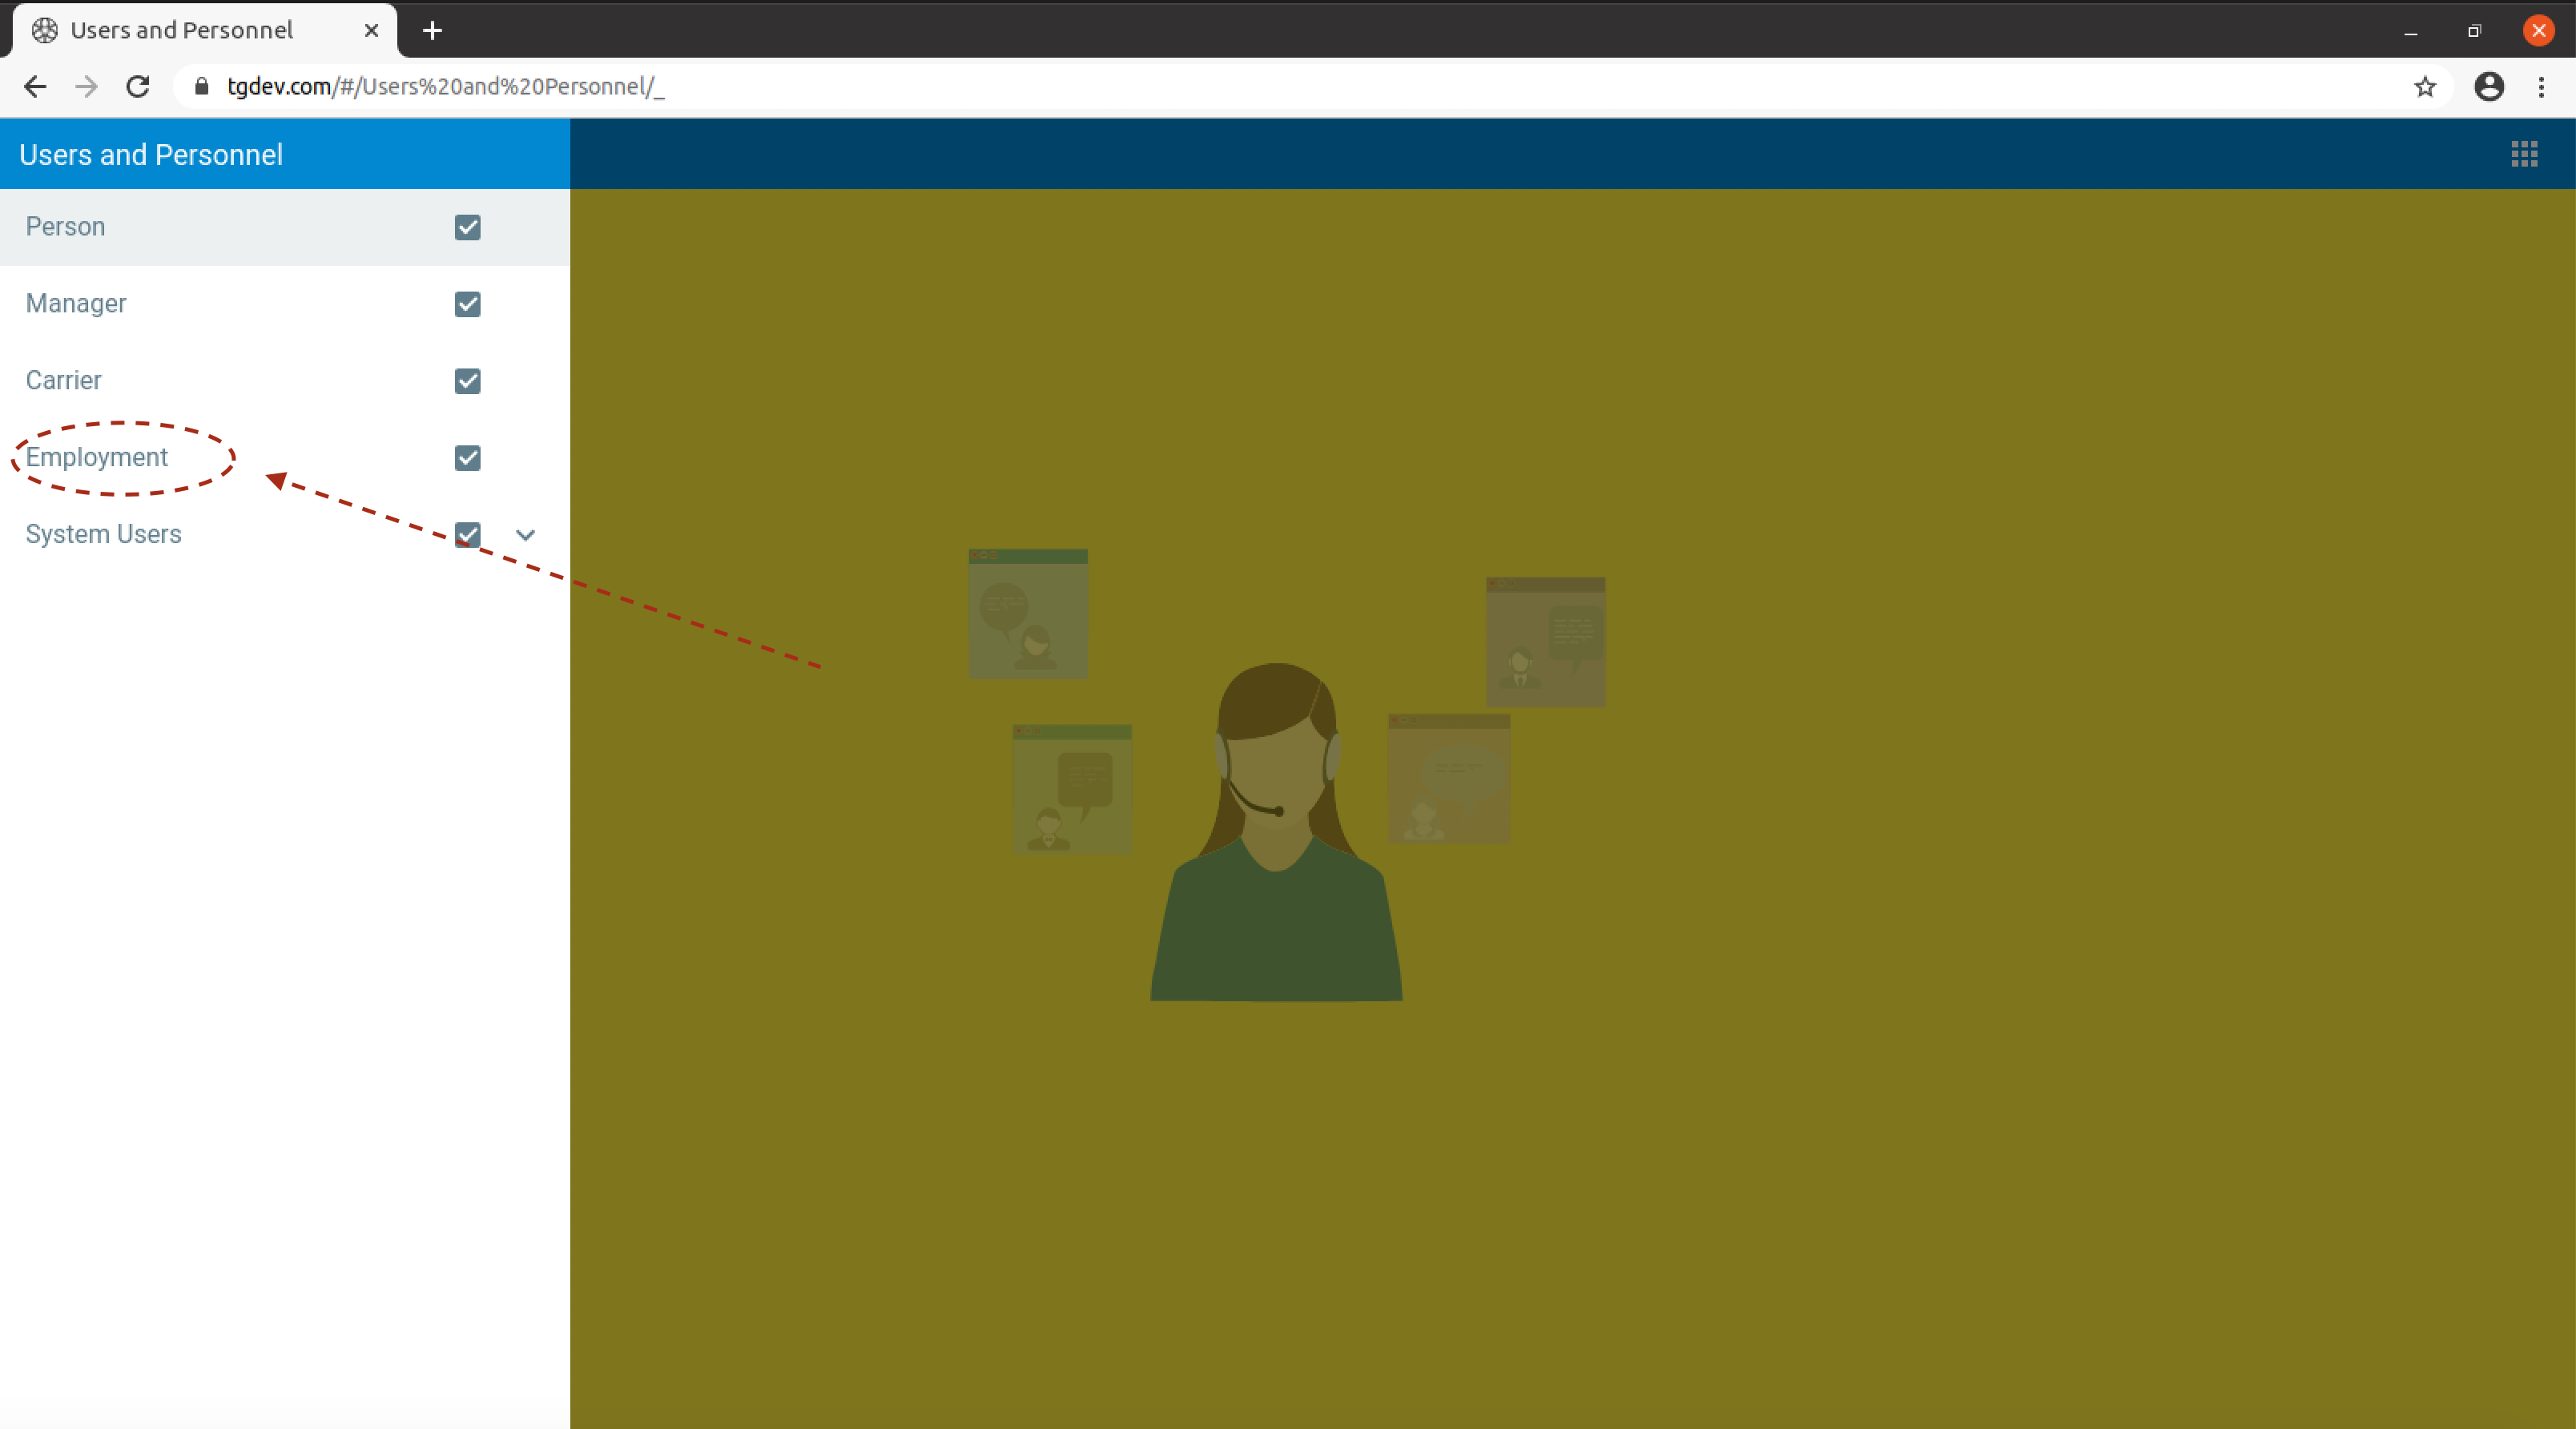
\includegraphics[width=\textwidth]{sections/01-chapter/images/employment11.png}

An employment entity can be found using the following properties:

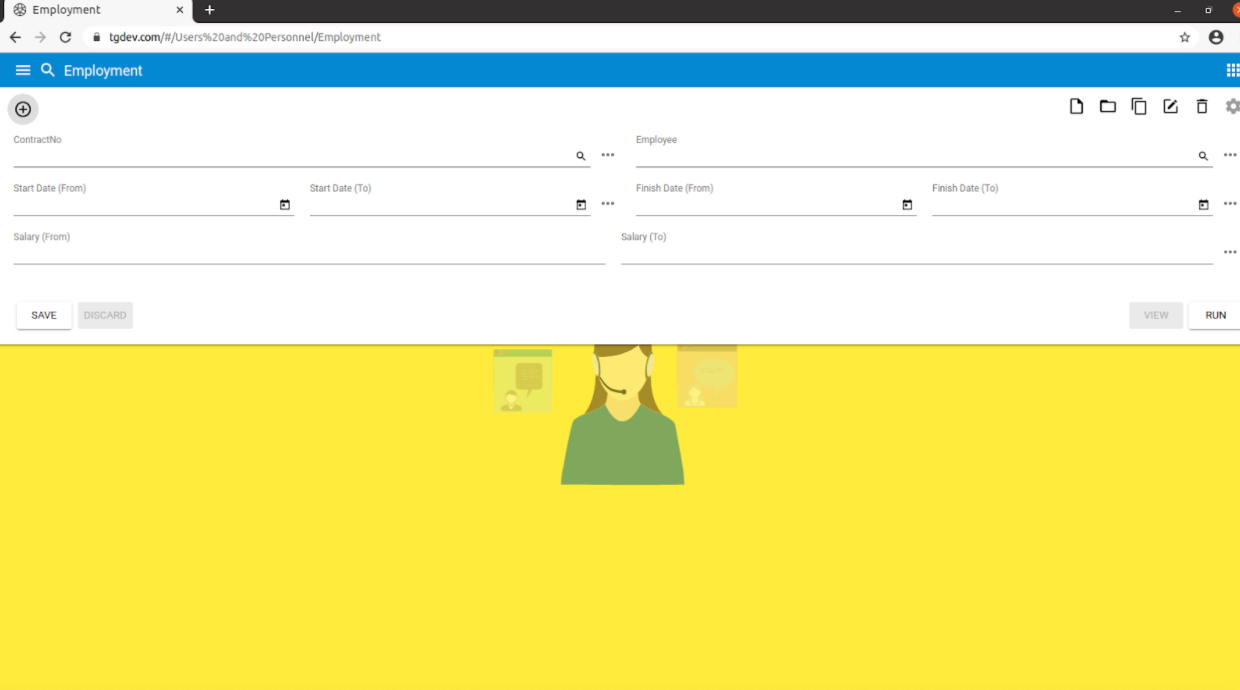
\includegraphics[width=\textwidth]{sections/01-chapter/images/employment2.png}

- ContractNo → String that represents the number of a Contract

- Employee → the initials of a Person Employed

- StartDate (To and From) → range of the starting date of the contract, in which all of the needed Employees will fall

- FinishDate (From and To) → the range of the Finish Dates where the needed employee contracts will fall

- Salary (To and From) → the range of salaries to search in

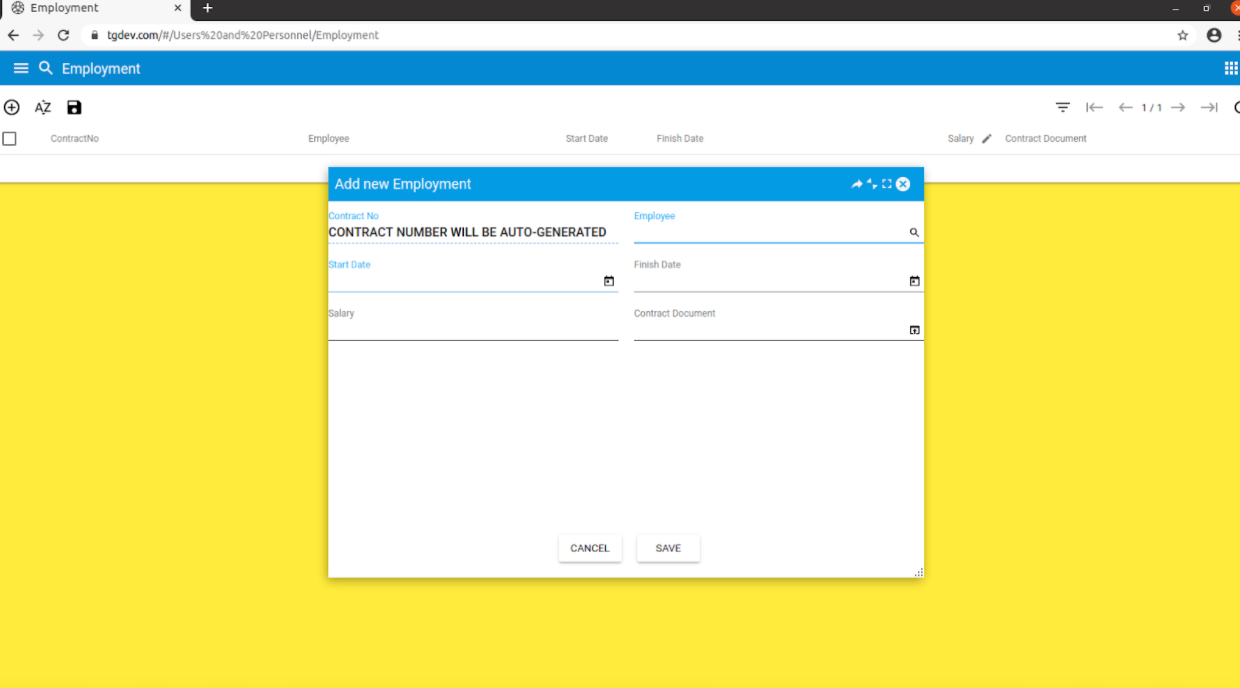
\includegraphics[width=\textwidth]{sections/01-chapter/images/employment3.png}

The registration of new Entity of Employment requires several fields:
- Contract Number - this field is generated automatically for your convenience and is not editable
- Employee - the initials of a person who is employed, required field

- Start Date - start date of the employment, required field

- Finish Date - finish date of the employment, optional field

- Salary - amount which is paid to the employee, optional field

- Contract Document - string that represents the hyperlink to the contract document, optional field

Fields  such as Employee and Start Date are required which means that they cannot be left empty, while Finish Date and Salary may be blank.

The Start and End Dates can be chosen from the popped up calendar icon:

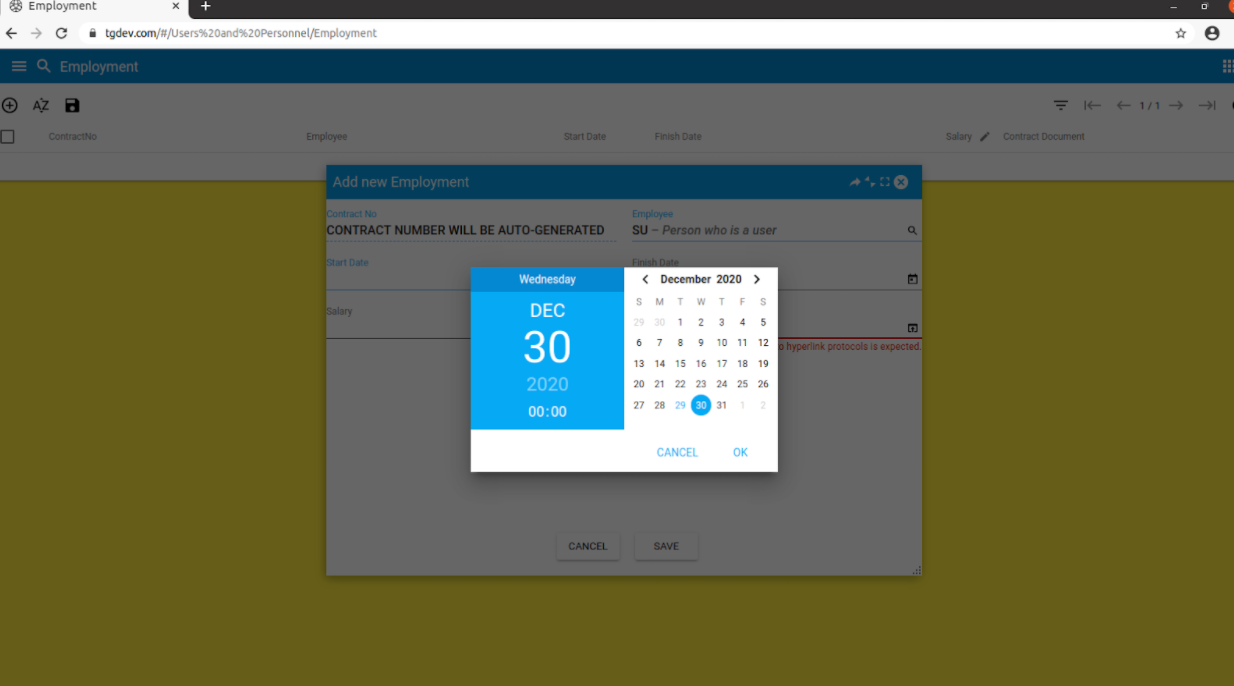
\includegraphics[width=\textwidth]{sections/01-chapter/images/employmentdates.png}

To save the entered information you need to click on the ‘Save’ button. 

To cancel the process and close the form to click on the ‘Cancel' button.

\section{Logistics}

Logistics section has the following roles: 

- Location 

- Order

- OrderItem

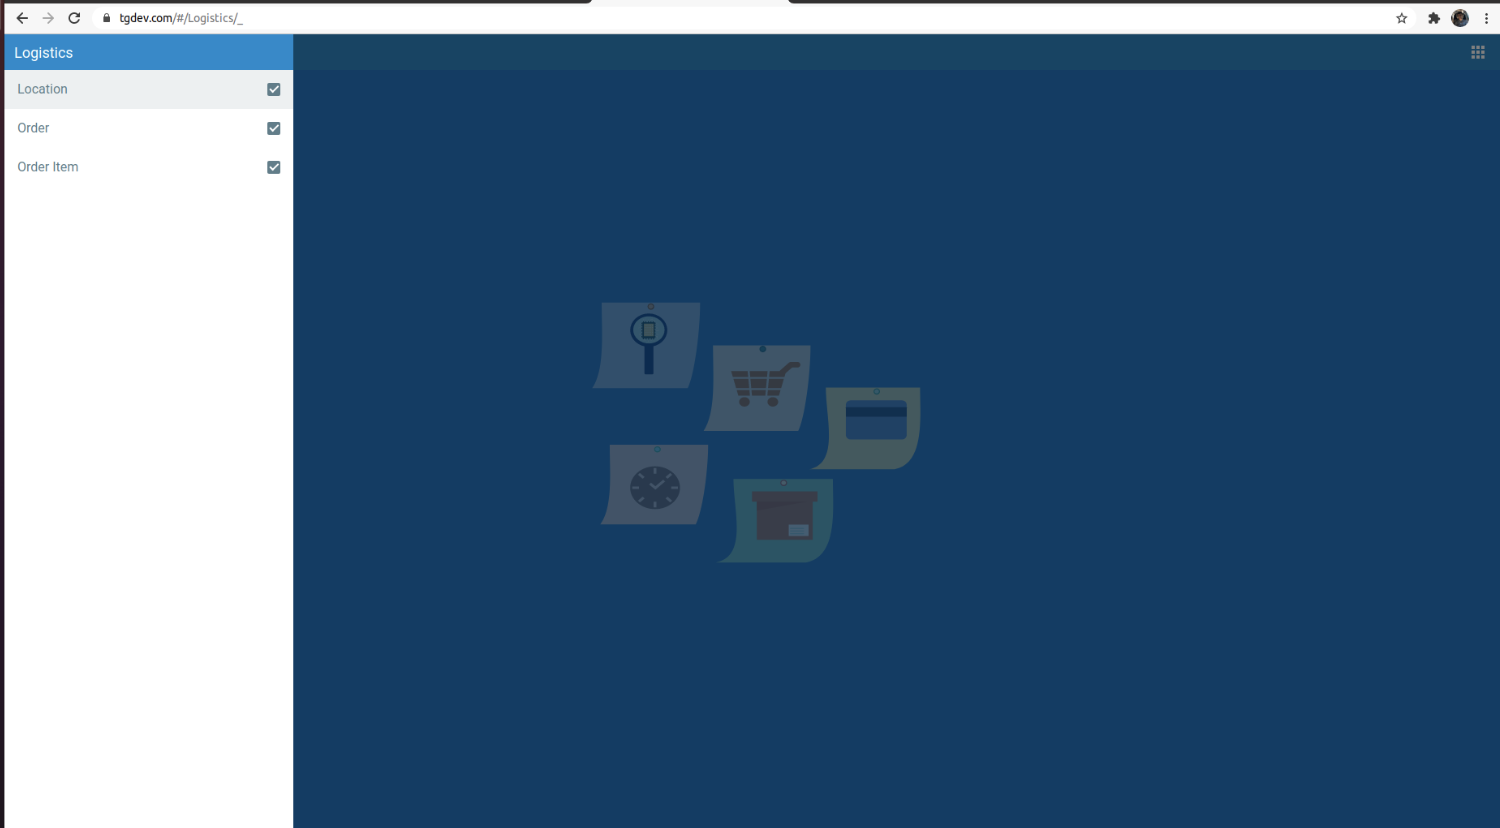
\includegraphics[width=\textwidth]{sections/01-chapter/images/logistics.png}

\subsection{Location}

The Location Entity represents a location where a bakery has one of its either distributing or production points. 

One can search through the list of register Location using the following fields:

- Location → the address of the Location

- Description → optional field, the description of the certain Location 

- Country of Location

- City of Location

- Address of Location

- Phone number on a Location

- Range of employee amount

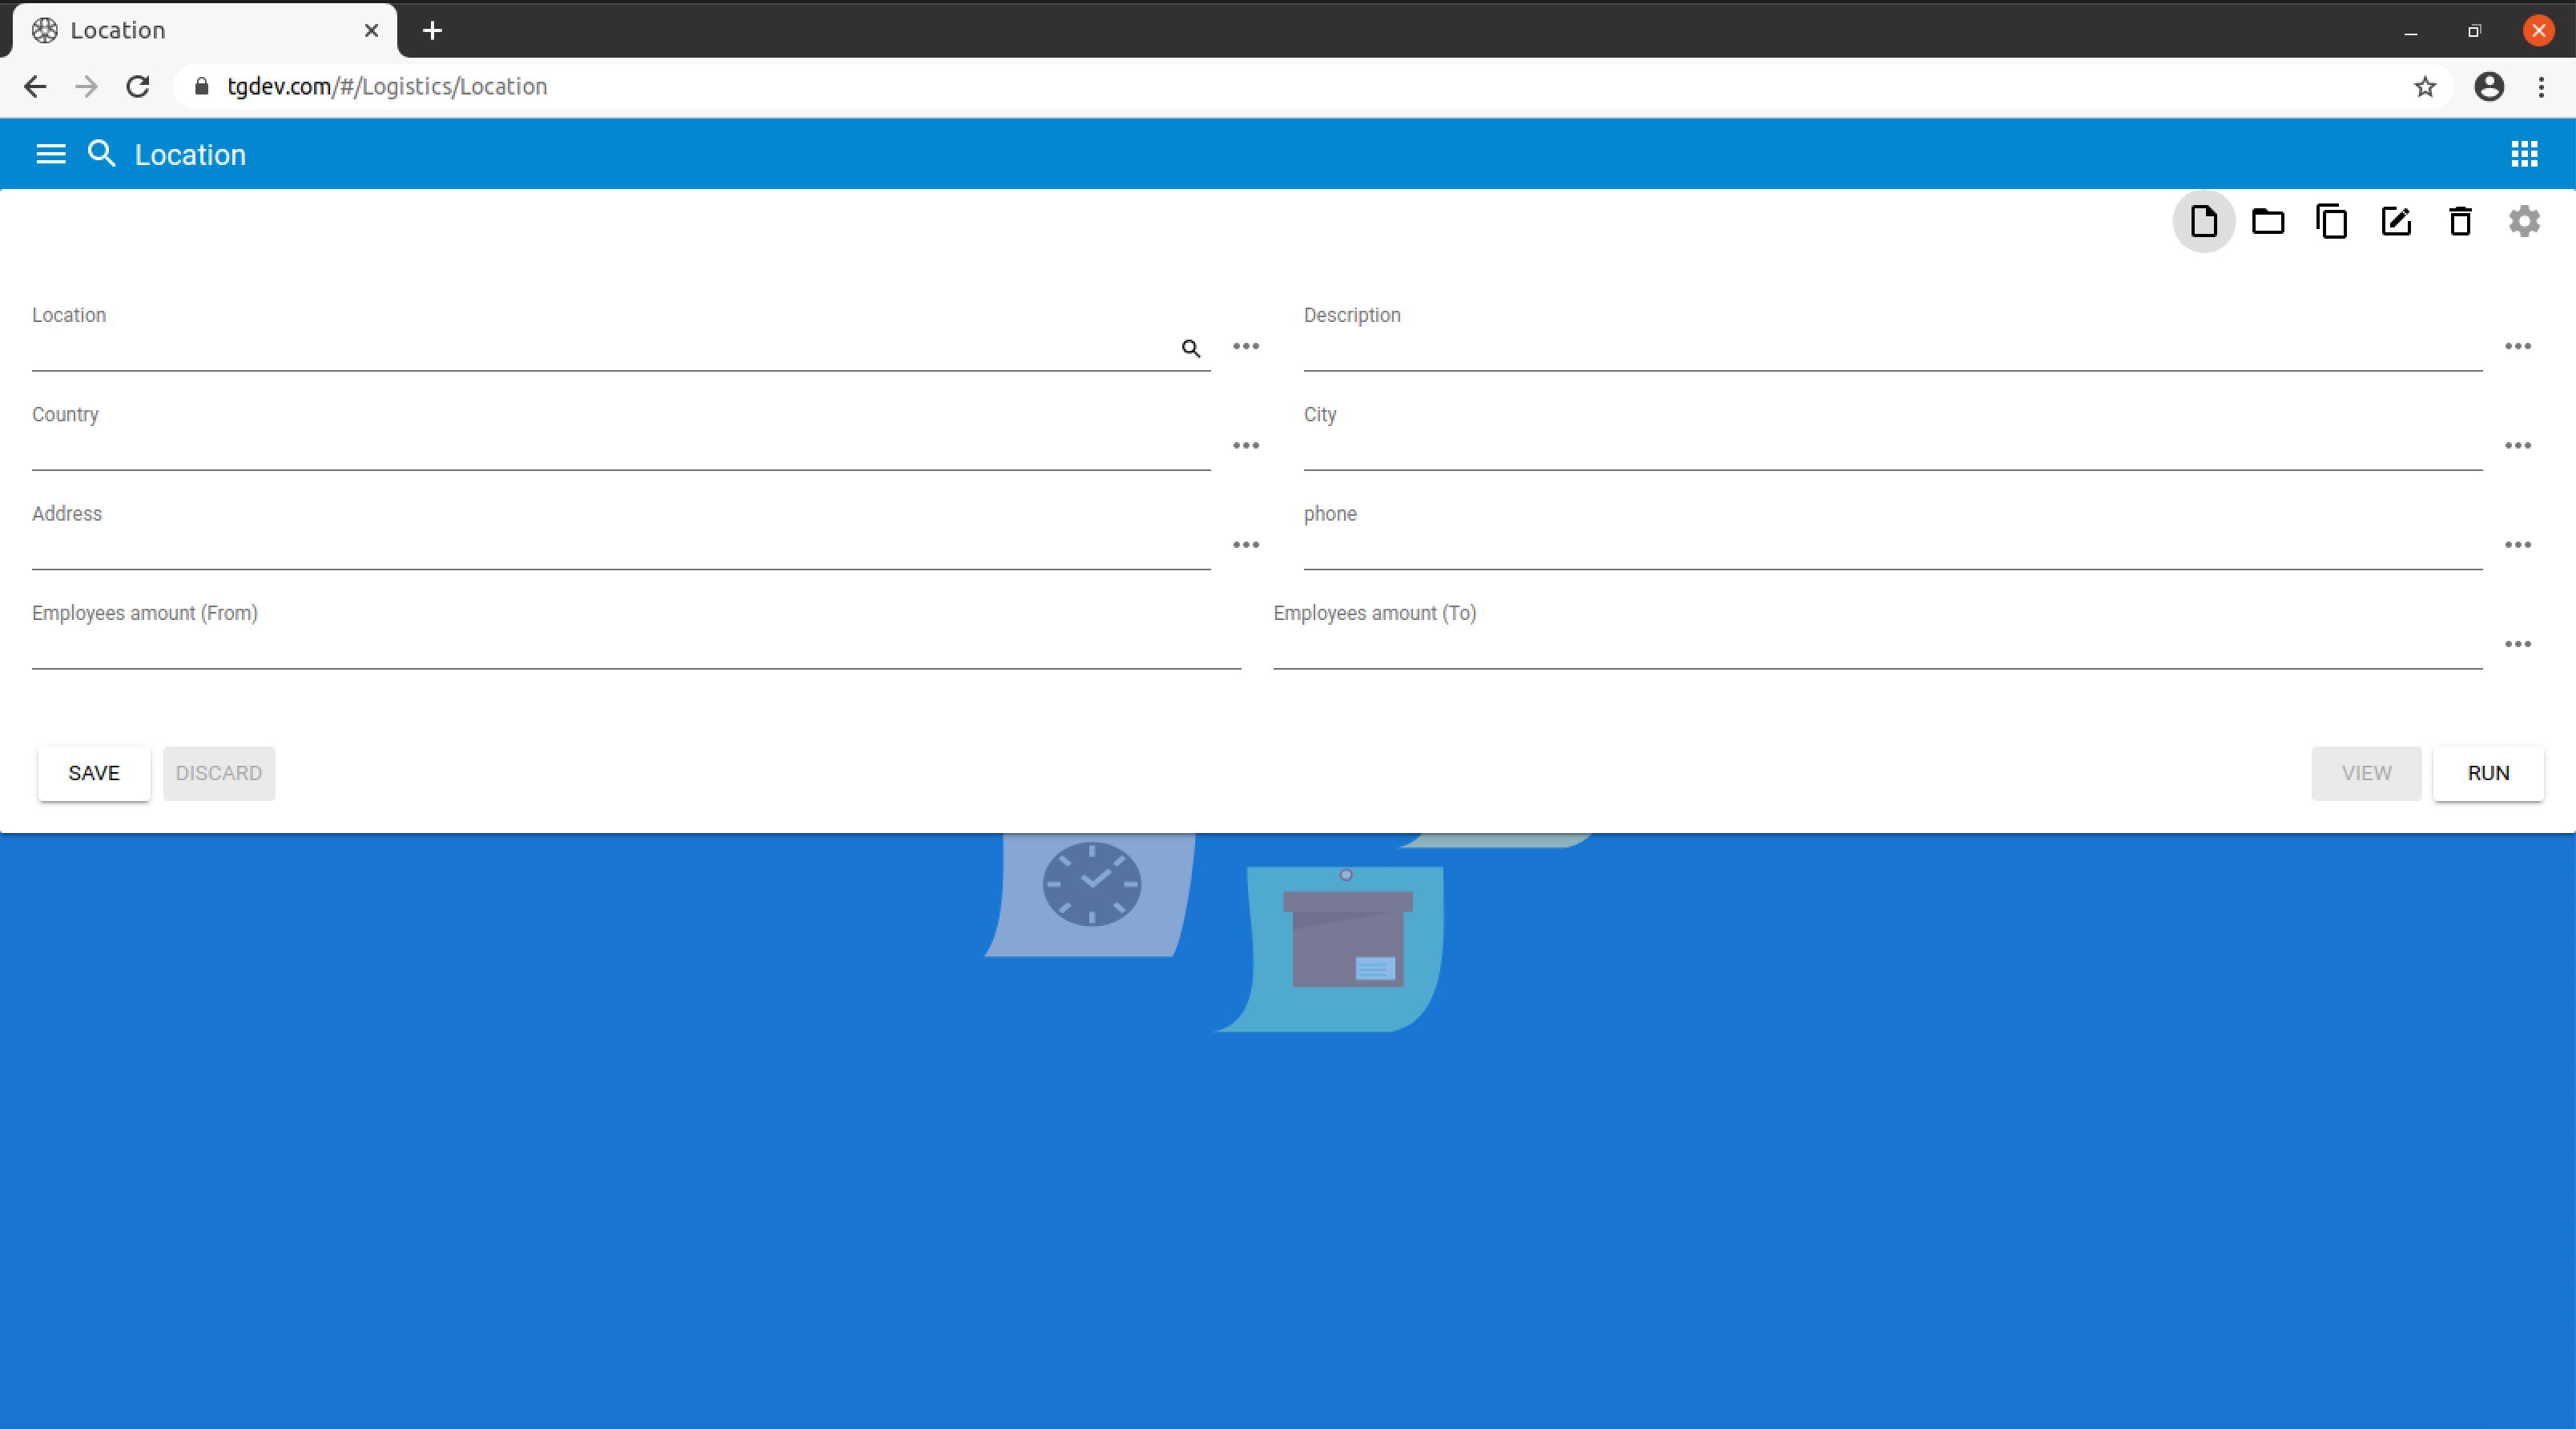
\includegraphics[width=\textwidth]{sections/01-chapter/images/location11.png}\\

For the registration of a new Location one should run the search and then press the + sign:

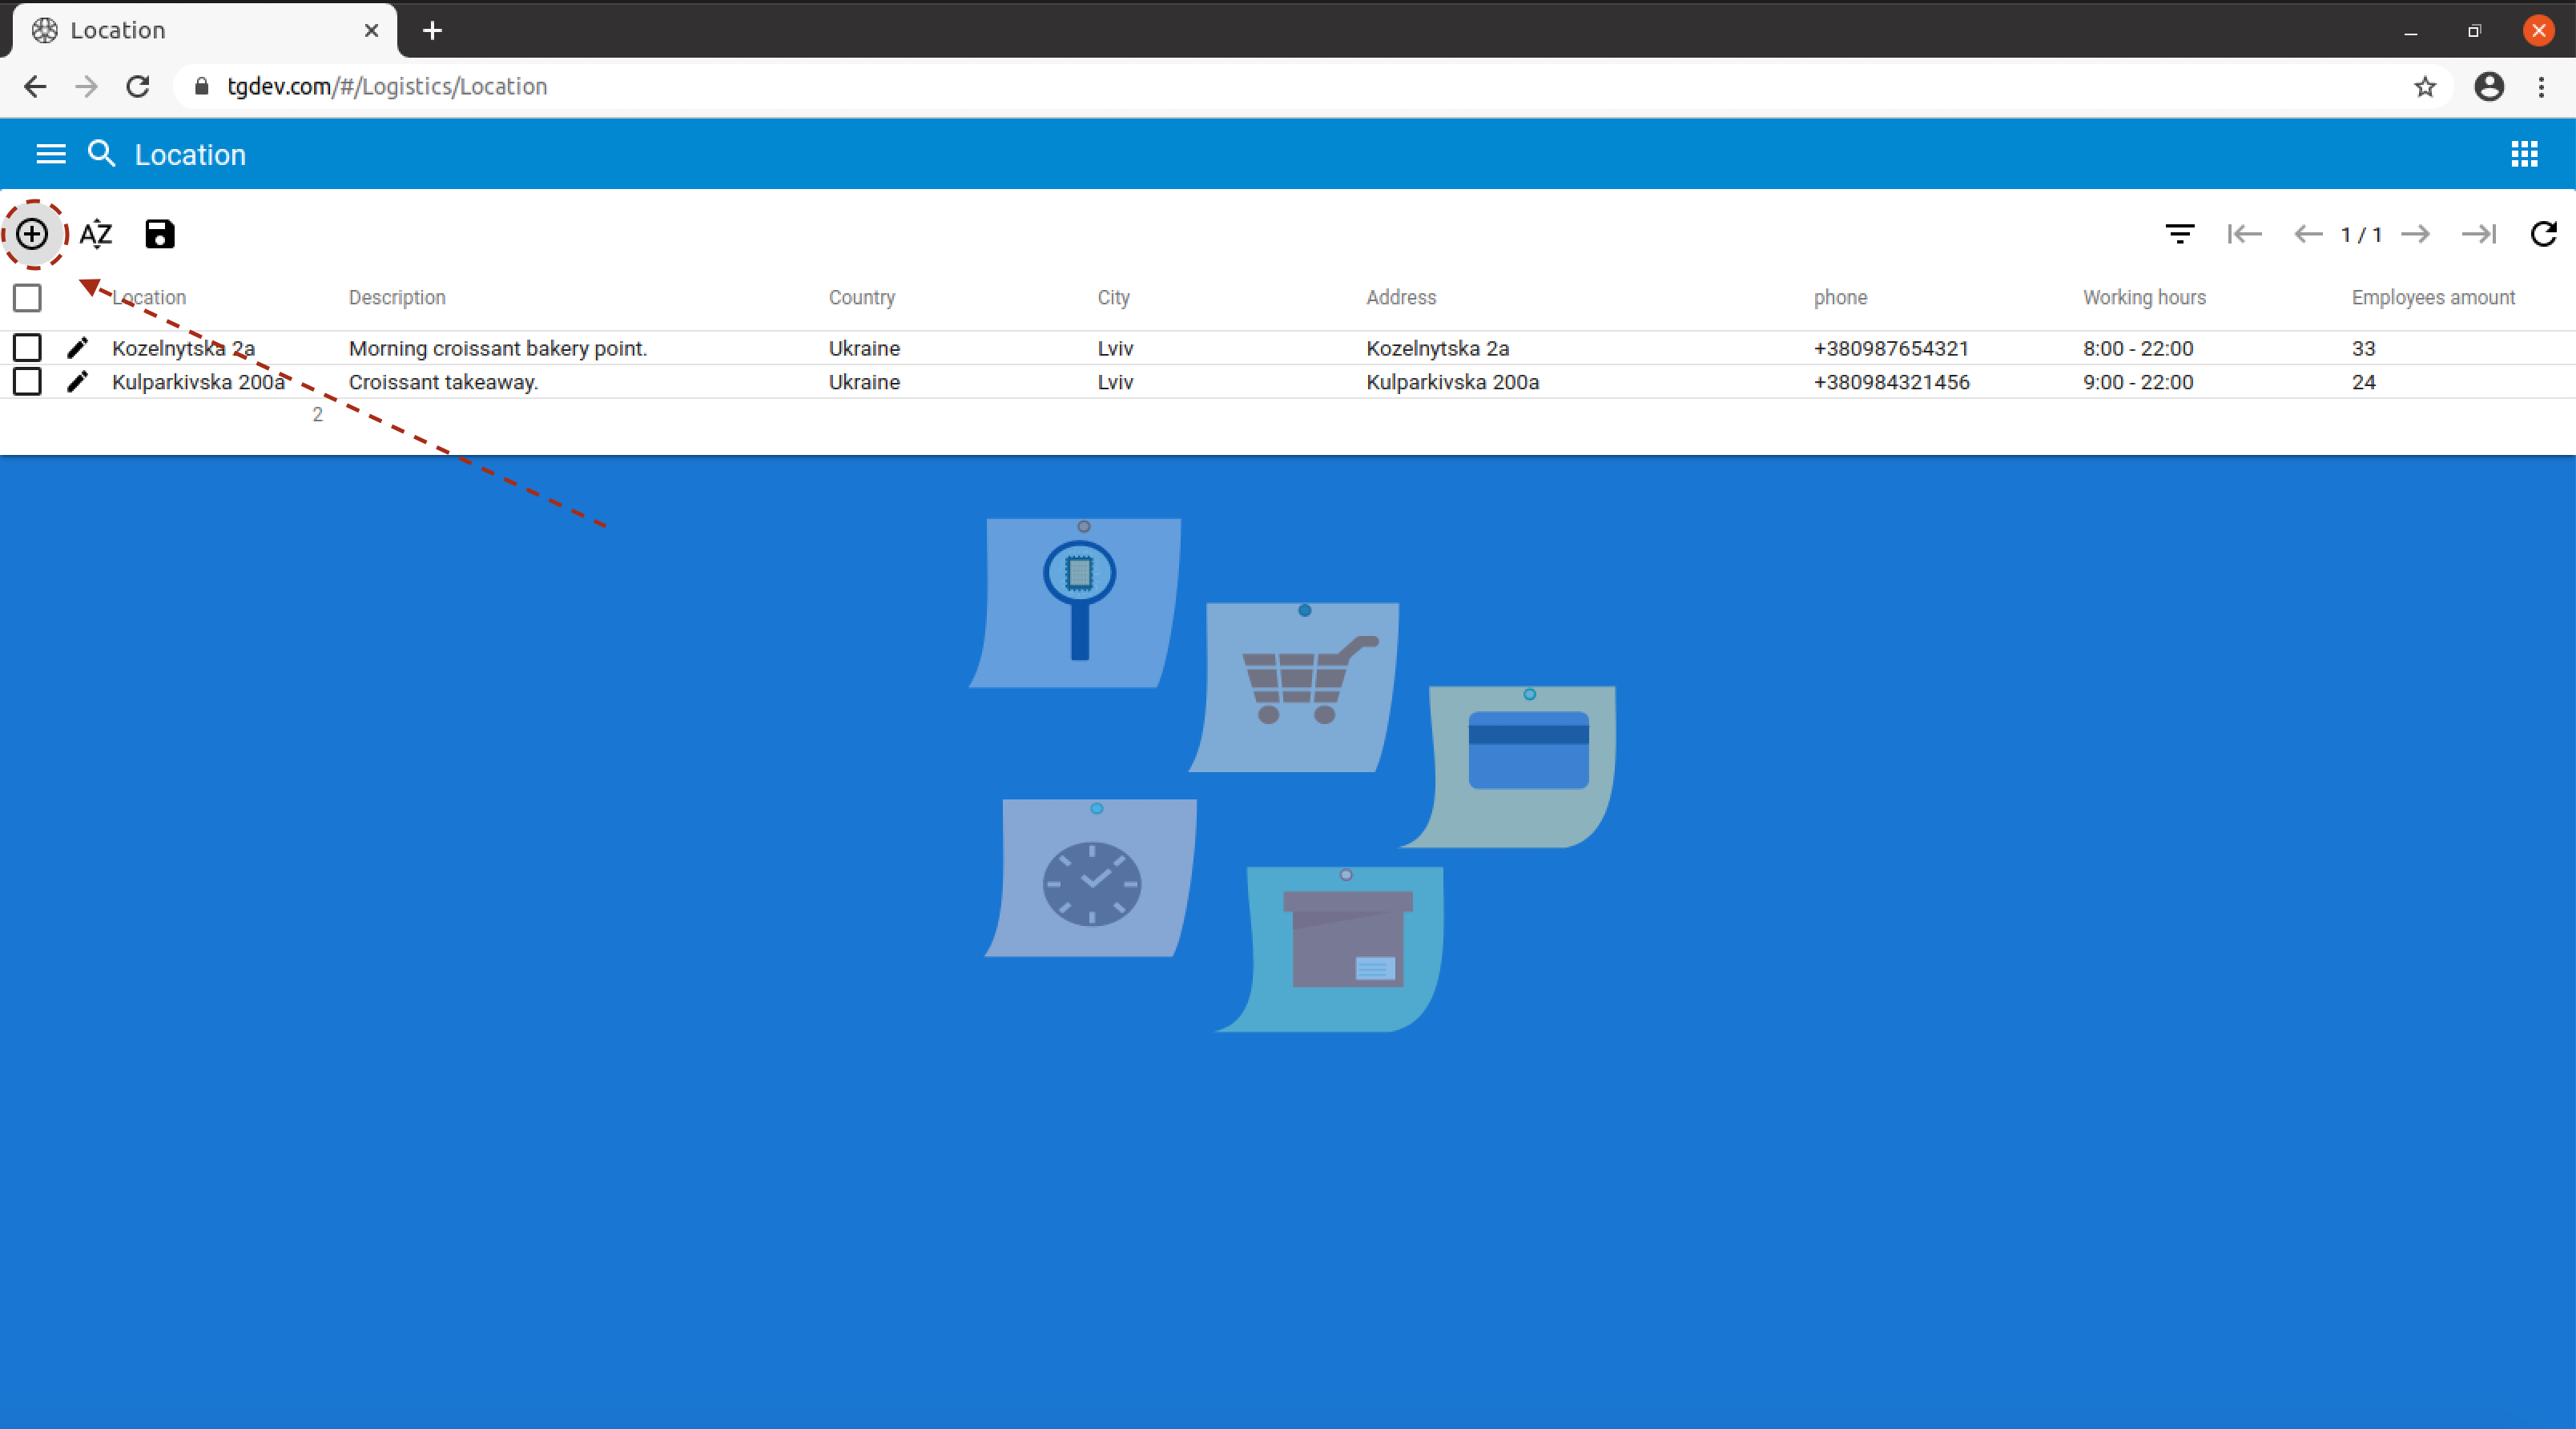
\includegraphics[width=\textwidth]{sections/01-chapter/images/location12.png}\\

The Entity depends on a variety of required information. The mandatory fields are highlighted blue and include:

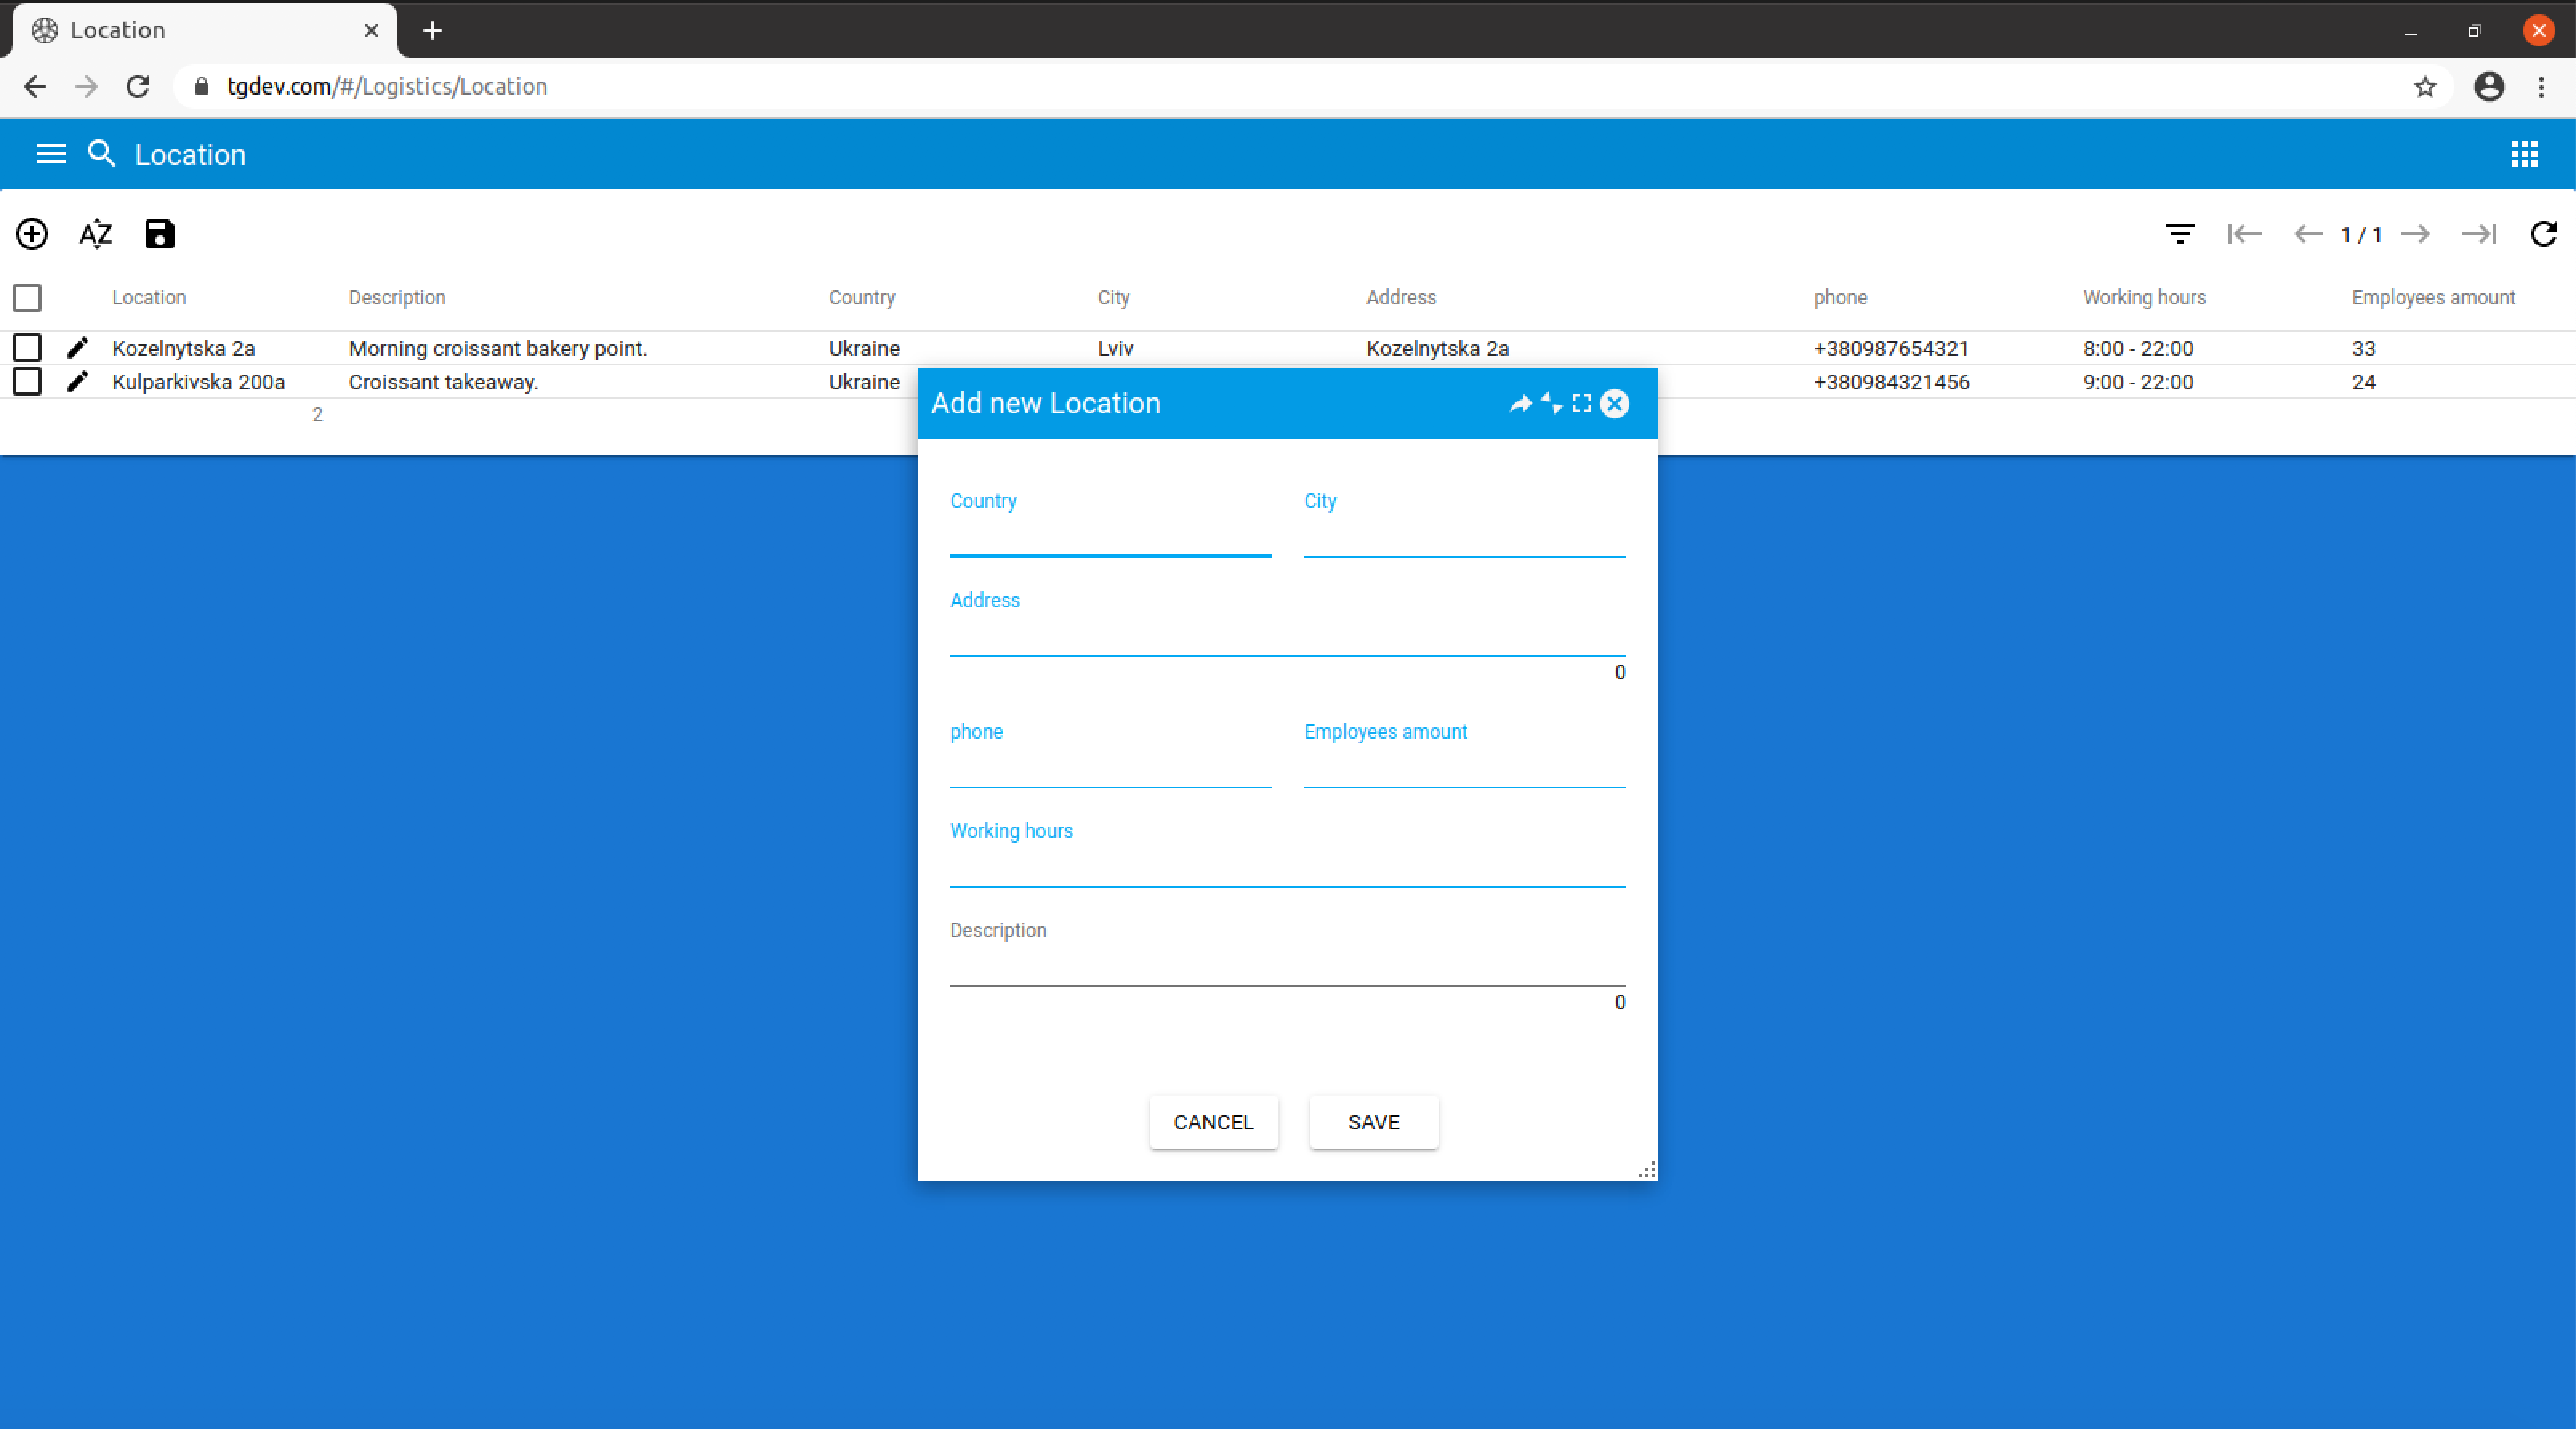
\includegraphics[width=\textwidth]{sections/01-chapter/images/location13.png}\\

- Country of the location → Required, String

- City → Required, String

- Address → Required, String that represents street and house number

- Phone → Required, String that represents the phone number of the location, letters are not permitted to be types in this field

- Employees amount → Required, Number that represents number of employees on the location

- Working hours → Required, String that represents the working hours of a location

The additional optional field is the description.


\subsection{Order}

The list of Orders is located as the rest of the entities -- in the left panel menu. 

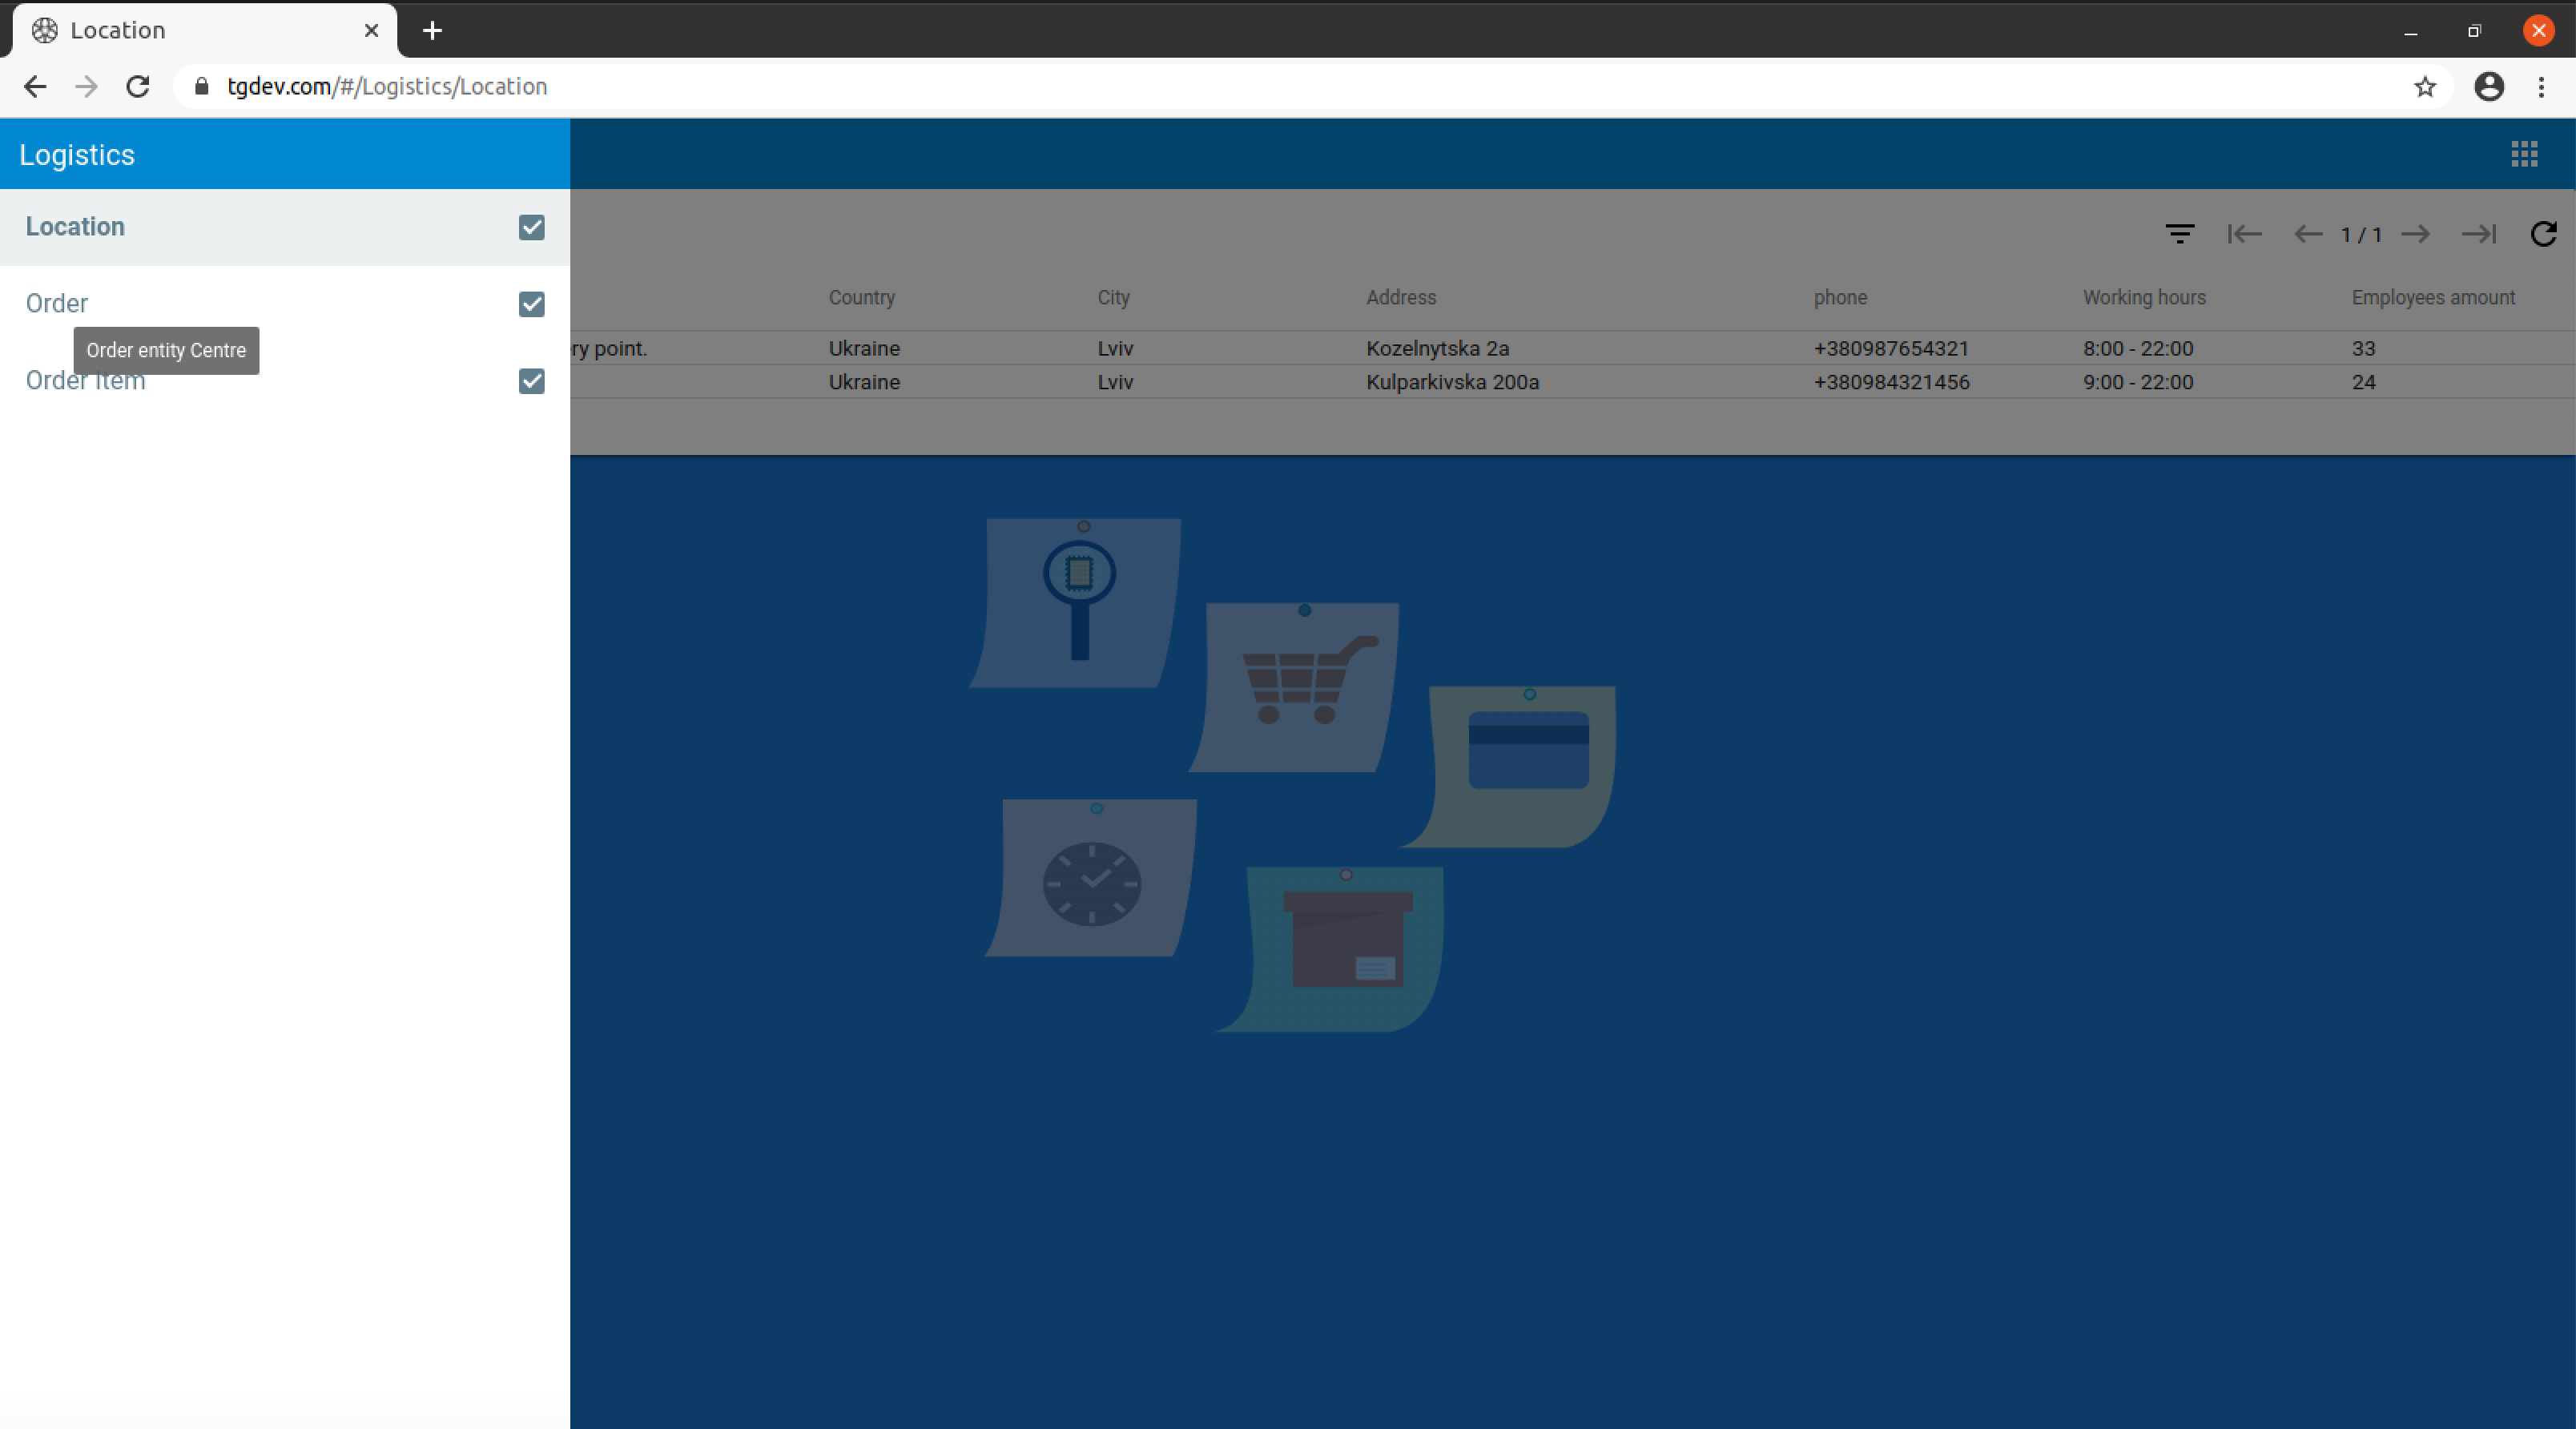
\includegraphics[width=\textwidth]{sections/01-chapter/images/order11.png}


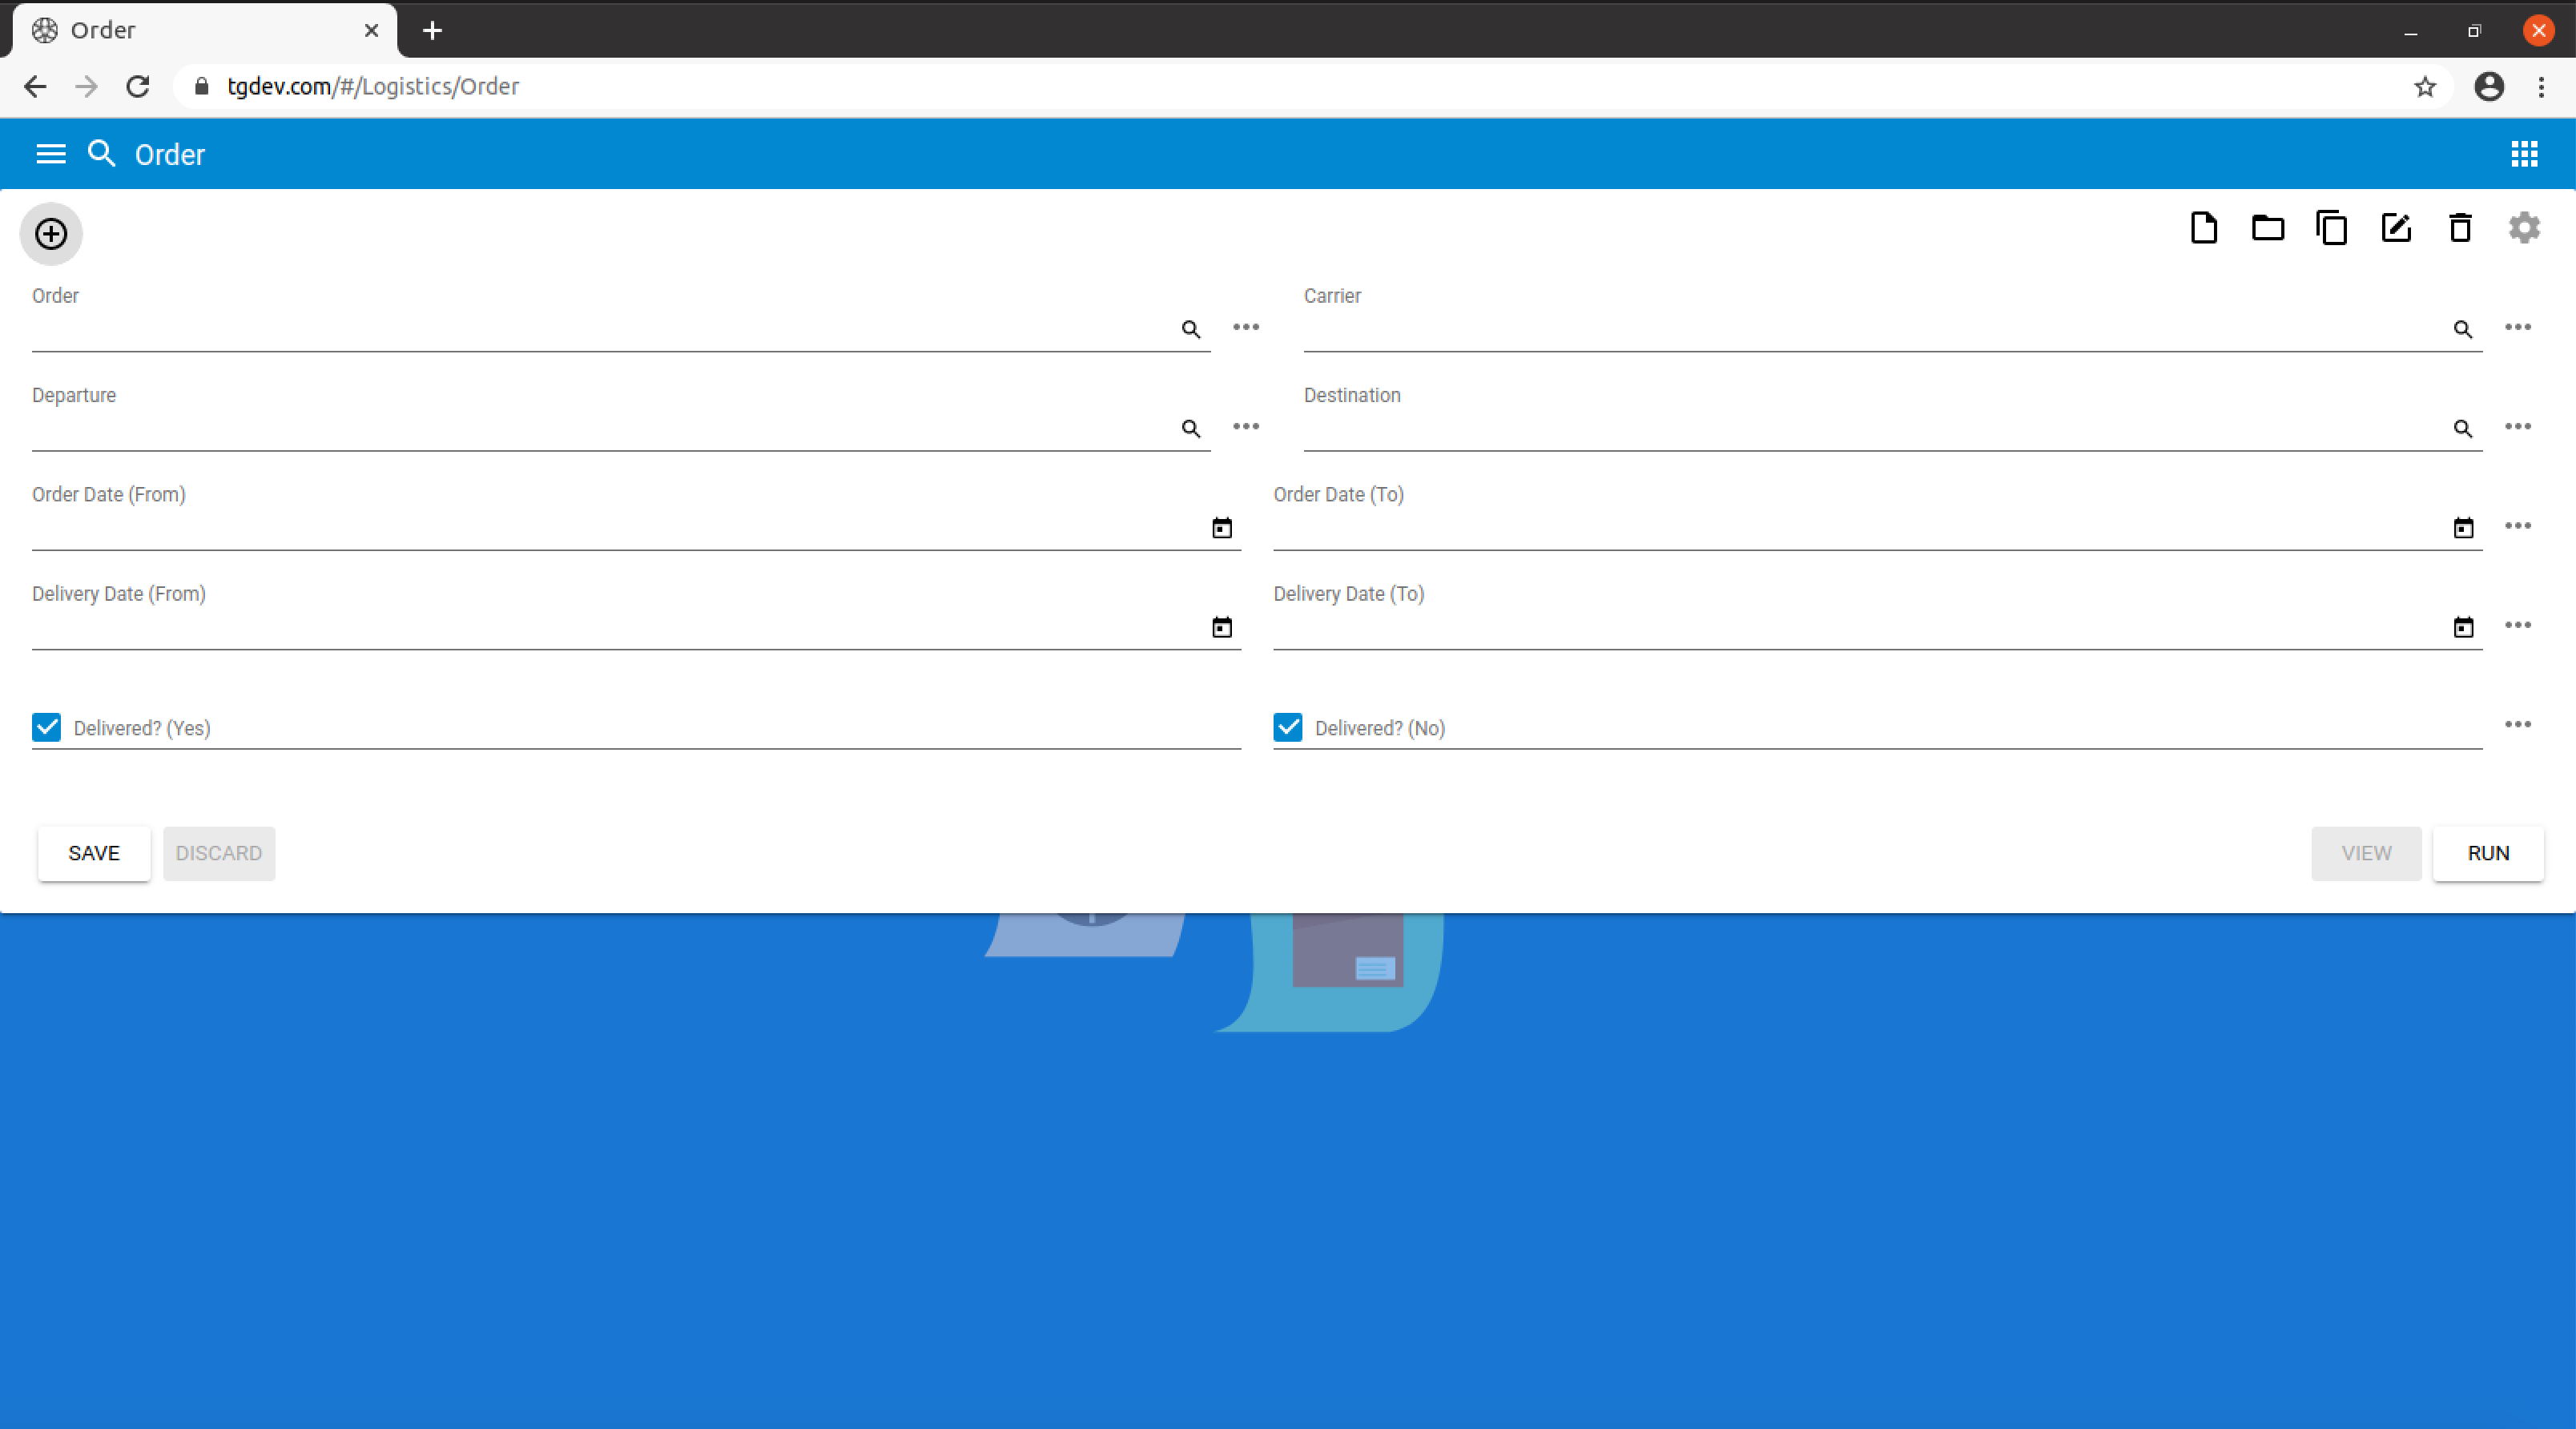
\includegraphics[width=\textwidth]{sections/01-chapter/images/order12.png}

The list of available orders in the System will be displayed as following:

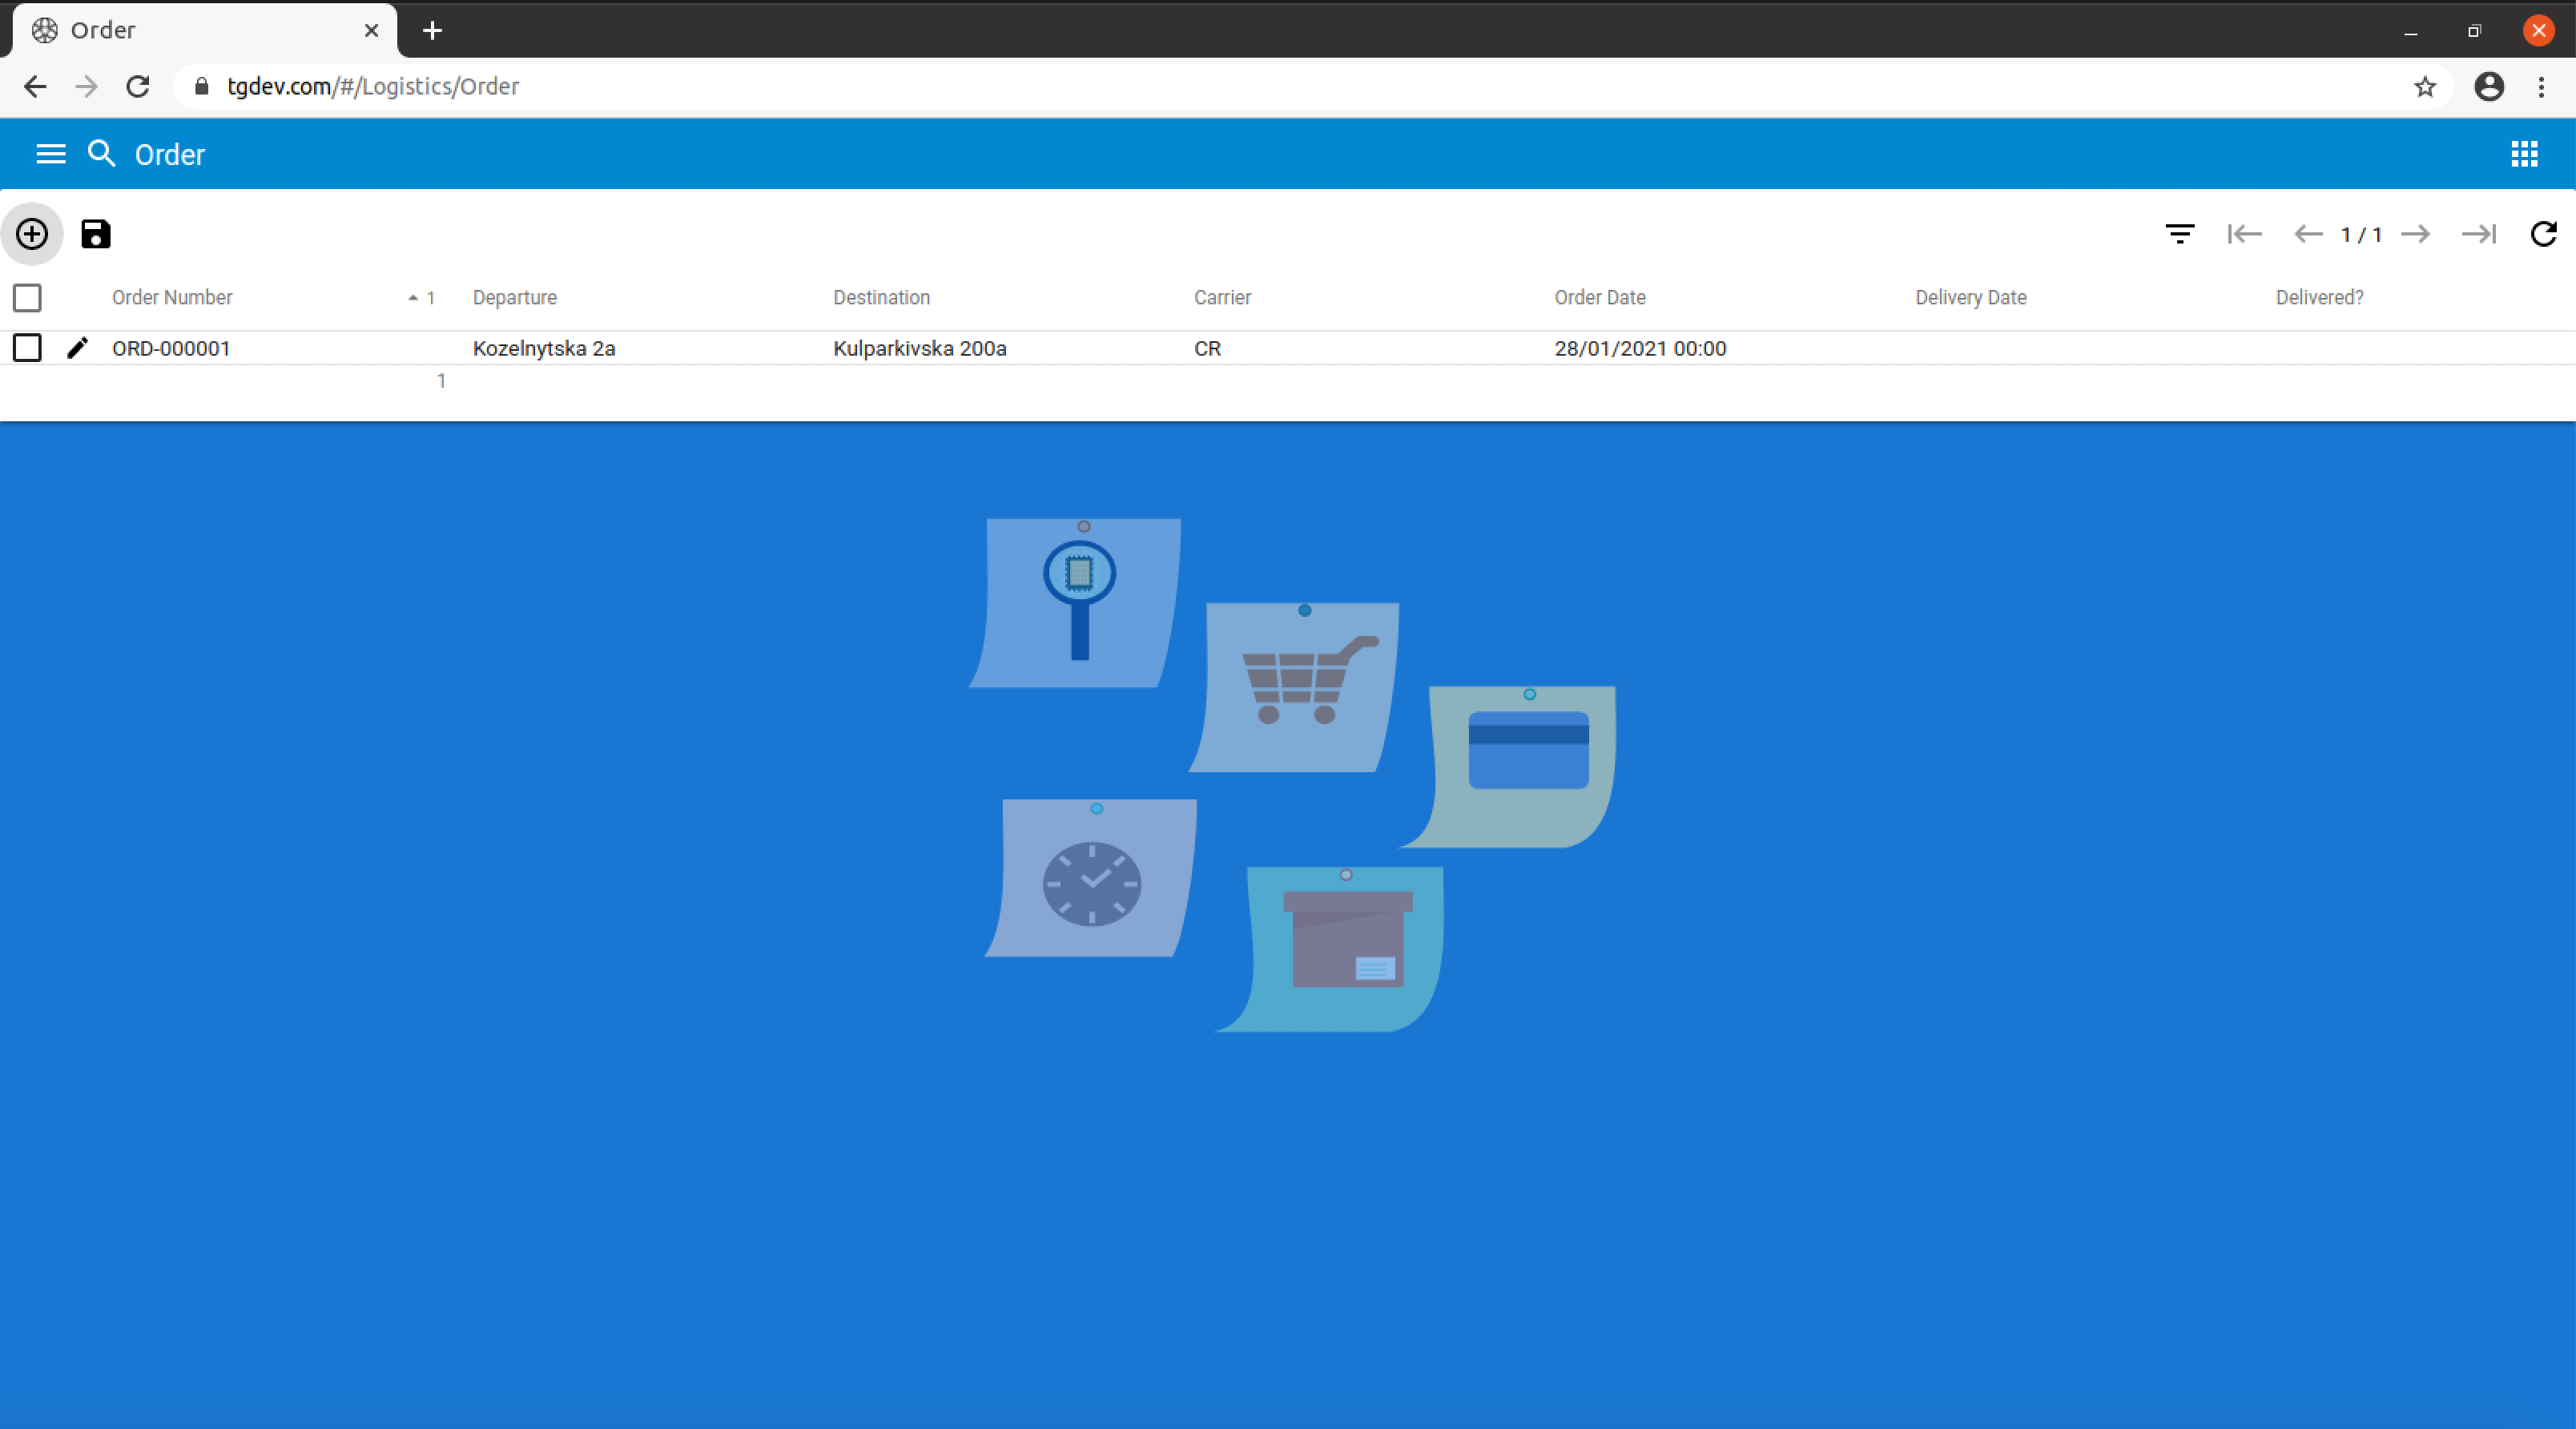
\includegraphics[width=\textwidth]{sections/01-chapter/images/order13.png}

Order has four columns which are the properties:

- orderNo → string that represents the order code number in the format "ORD-OOOOOOO".By default it is automatically generated, but can be set up by User during man

- Carrier → String that represents the initials of a  Carrier, a person in the carrier position who will be responsible for delivering an order.

- LocationFrom → the location from which the order will be delivered

- LocationTo → the location to which the order will be delivered

- Delivered ? - boolean checkbox, which indicated True if ordered is delivered an false otherwise

- orderDate  →  date when the order was made

- deliveryDate  → date when the order was delivered to LocationTo, it will be set automatically to current date when delivered checkbox is clicked


During the adding of new Order the list of available Locations to choose from will be proposed. The Carrier can be chosen from the list of available Carriers in the system.
Important things: The LocationFrom and LocationTo fields cannot be the same.


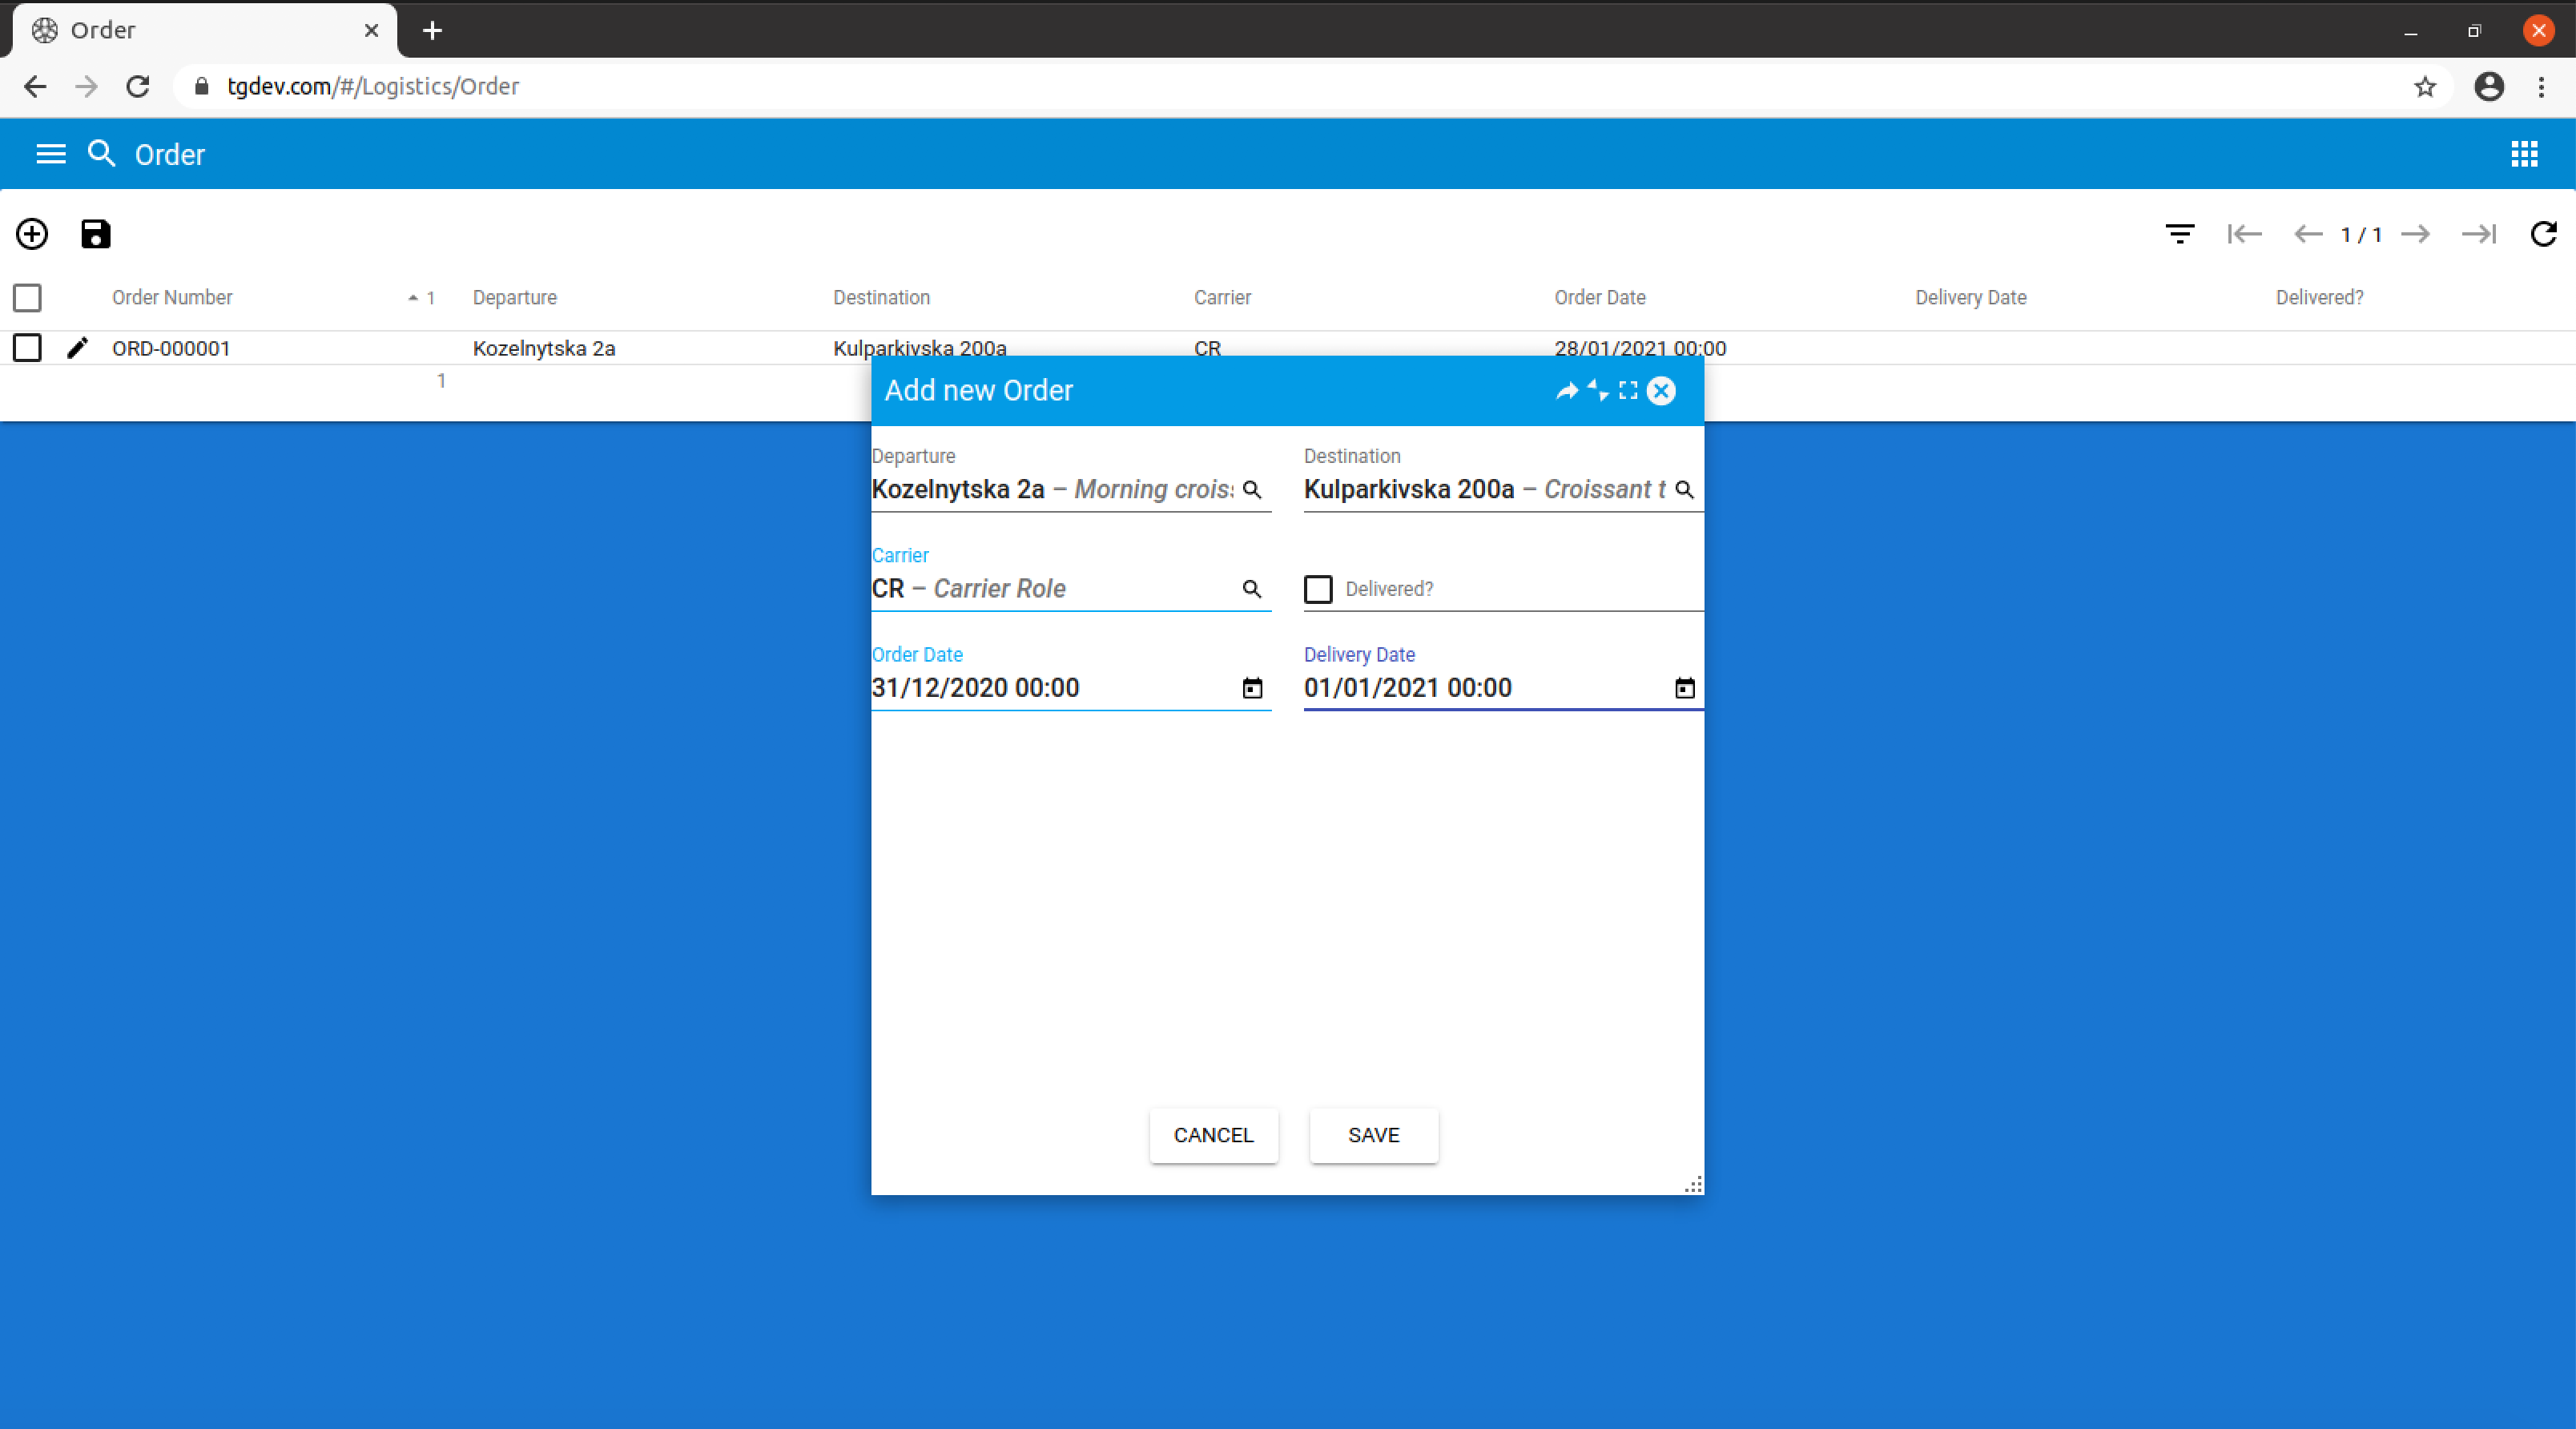
\includegraphics[width=\textwidth]{sections/01-chapter/images/order14.png}

\subsection{OrderItem}

After adding the Order to the database, You can edit the content of Order using the OrderItem Entity. The OrderItem entity describes the relationship between an Order and the Products in that Entity. 

In order to add a new OrderItem entity one should choose an Order which it wants to edit using order number, and choose the Product that belongs to the chosen Order from the list of available products and the quantity of the Product. 

So, OrderItem has the following fields/properties:


- Order →  required fields which represents the order to which content will be added to.

- Product →  required field which represents the products which will be added to this order.

- Quantity →  required, integer which represents the quantity of product ordered.


For example, if a User has created an Order with the following parameters:

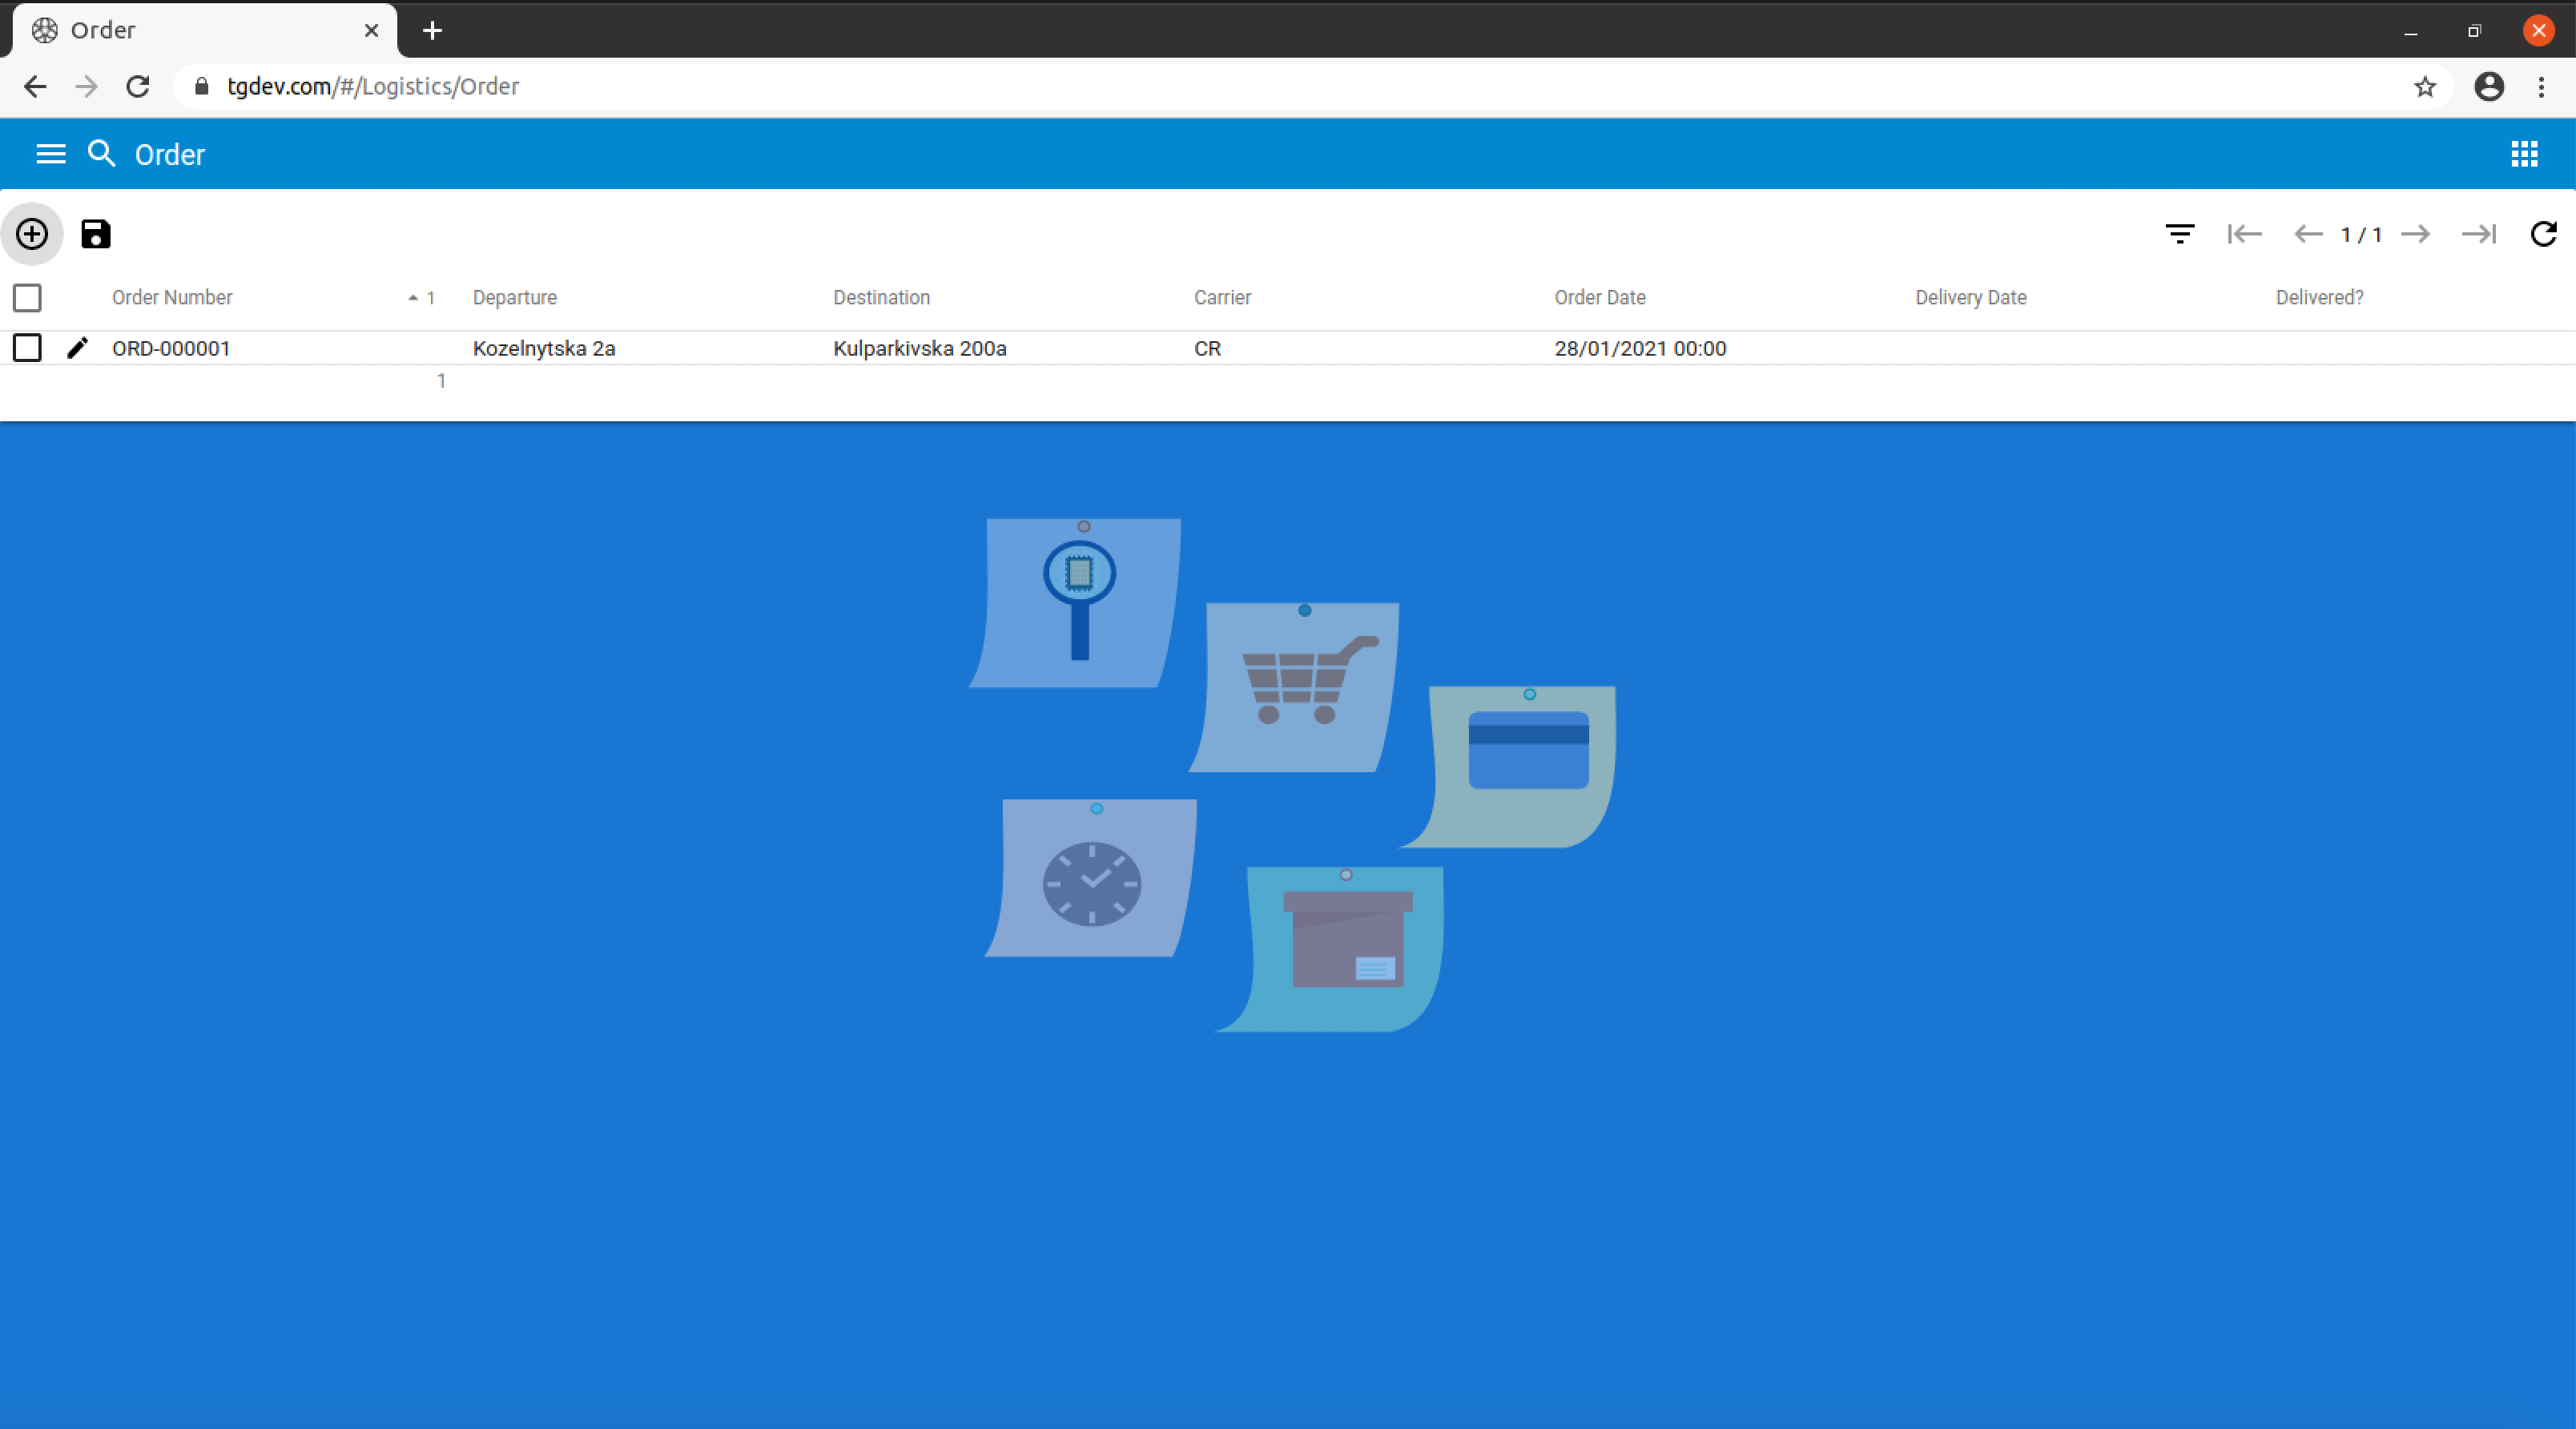
\includegraphics[width=\textwidth]{sections/01-chapter/images/order13.png}

Then they can add the content of that Order using OrderItem Entity. Let the Order under id ORD-000001 from Kozelnytska, 2a to Kulparkivska, 200a on 28.12.2020 00:00 contain the Products : Croissant with chocolate 150  pieces and Napoleon cake 10 pieces. 

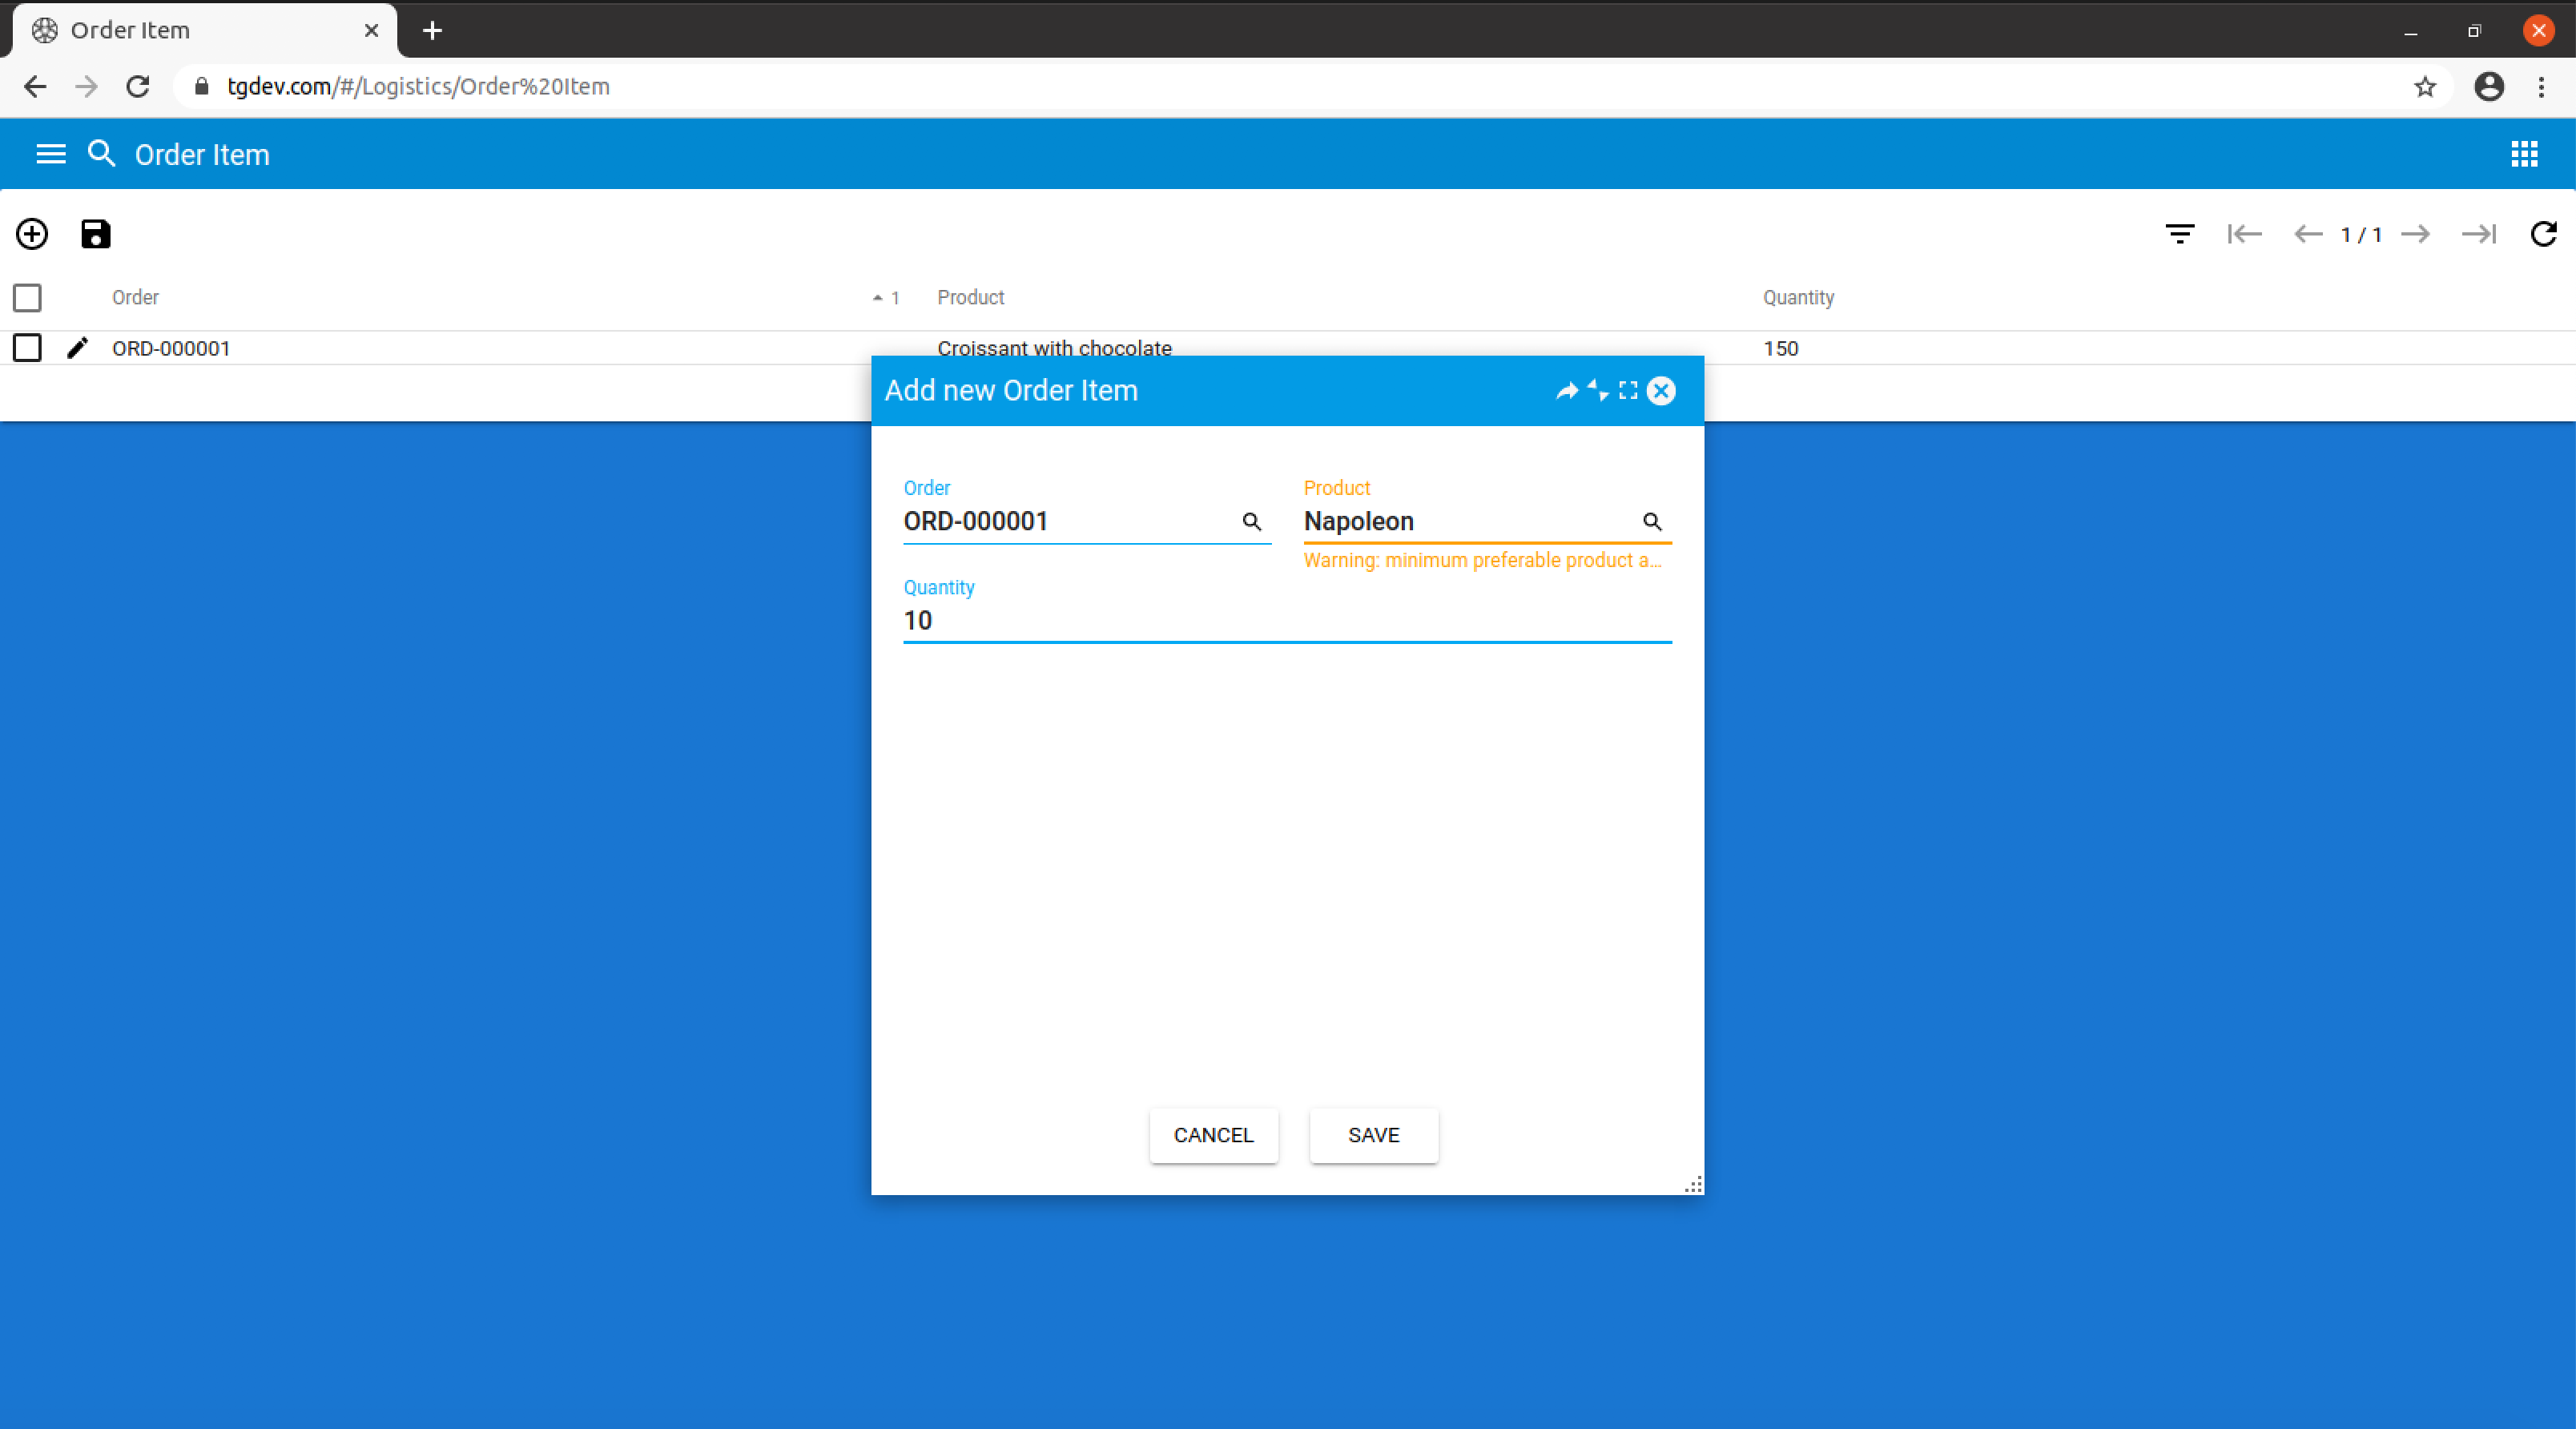
\includegraphics[width=\textwidth]{sections/01-chapter/images/orderitem12.png}


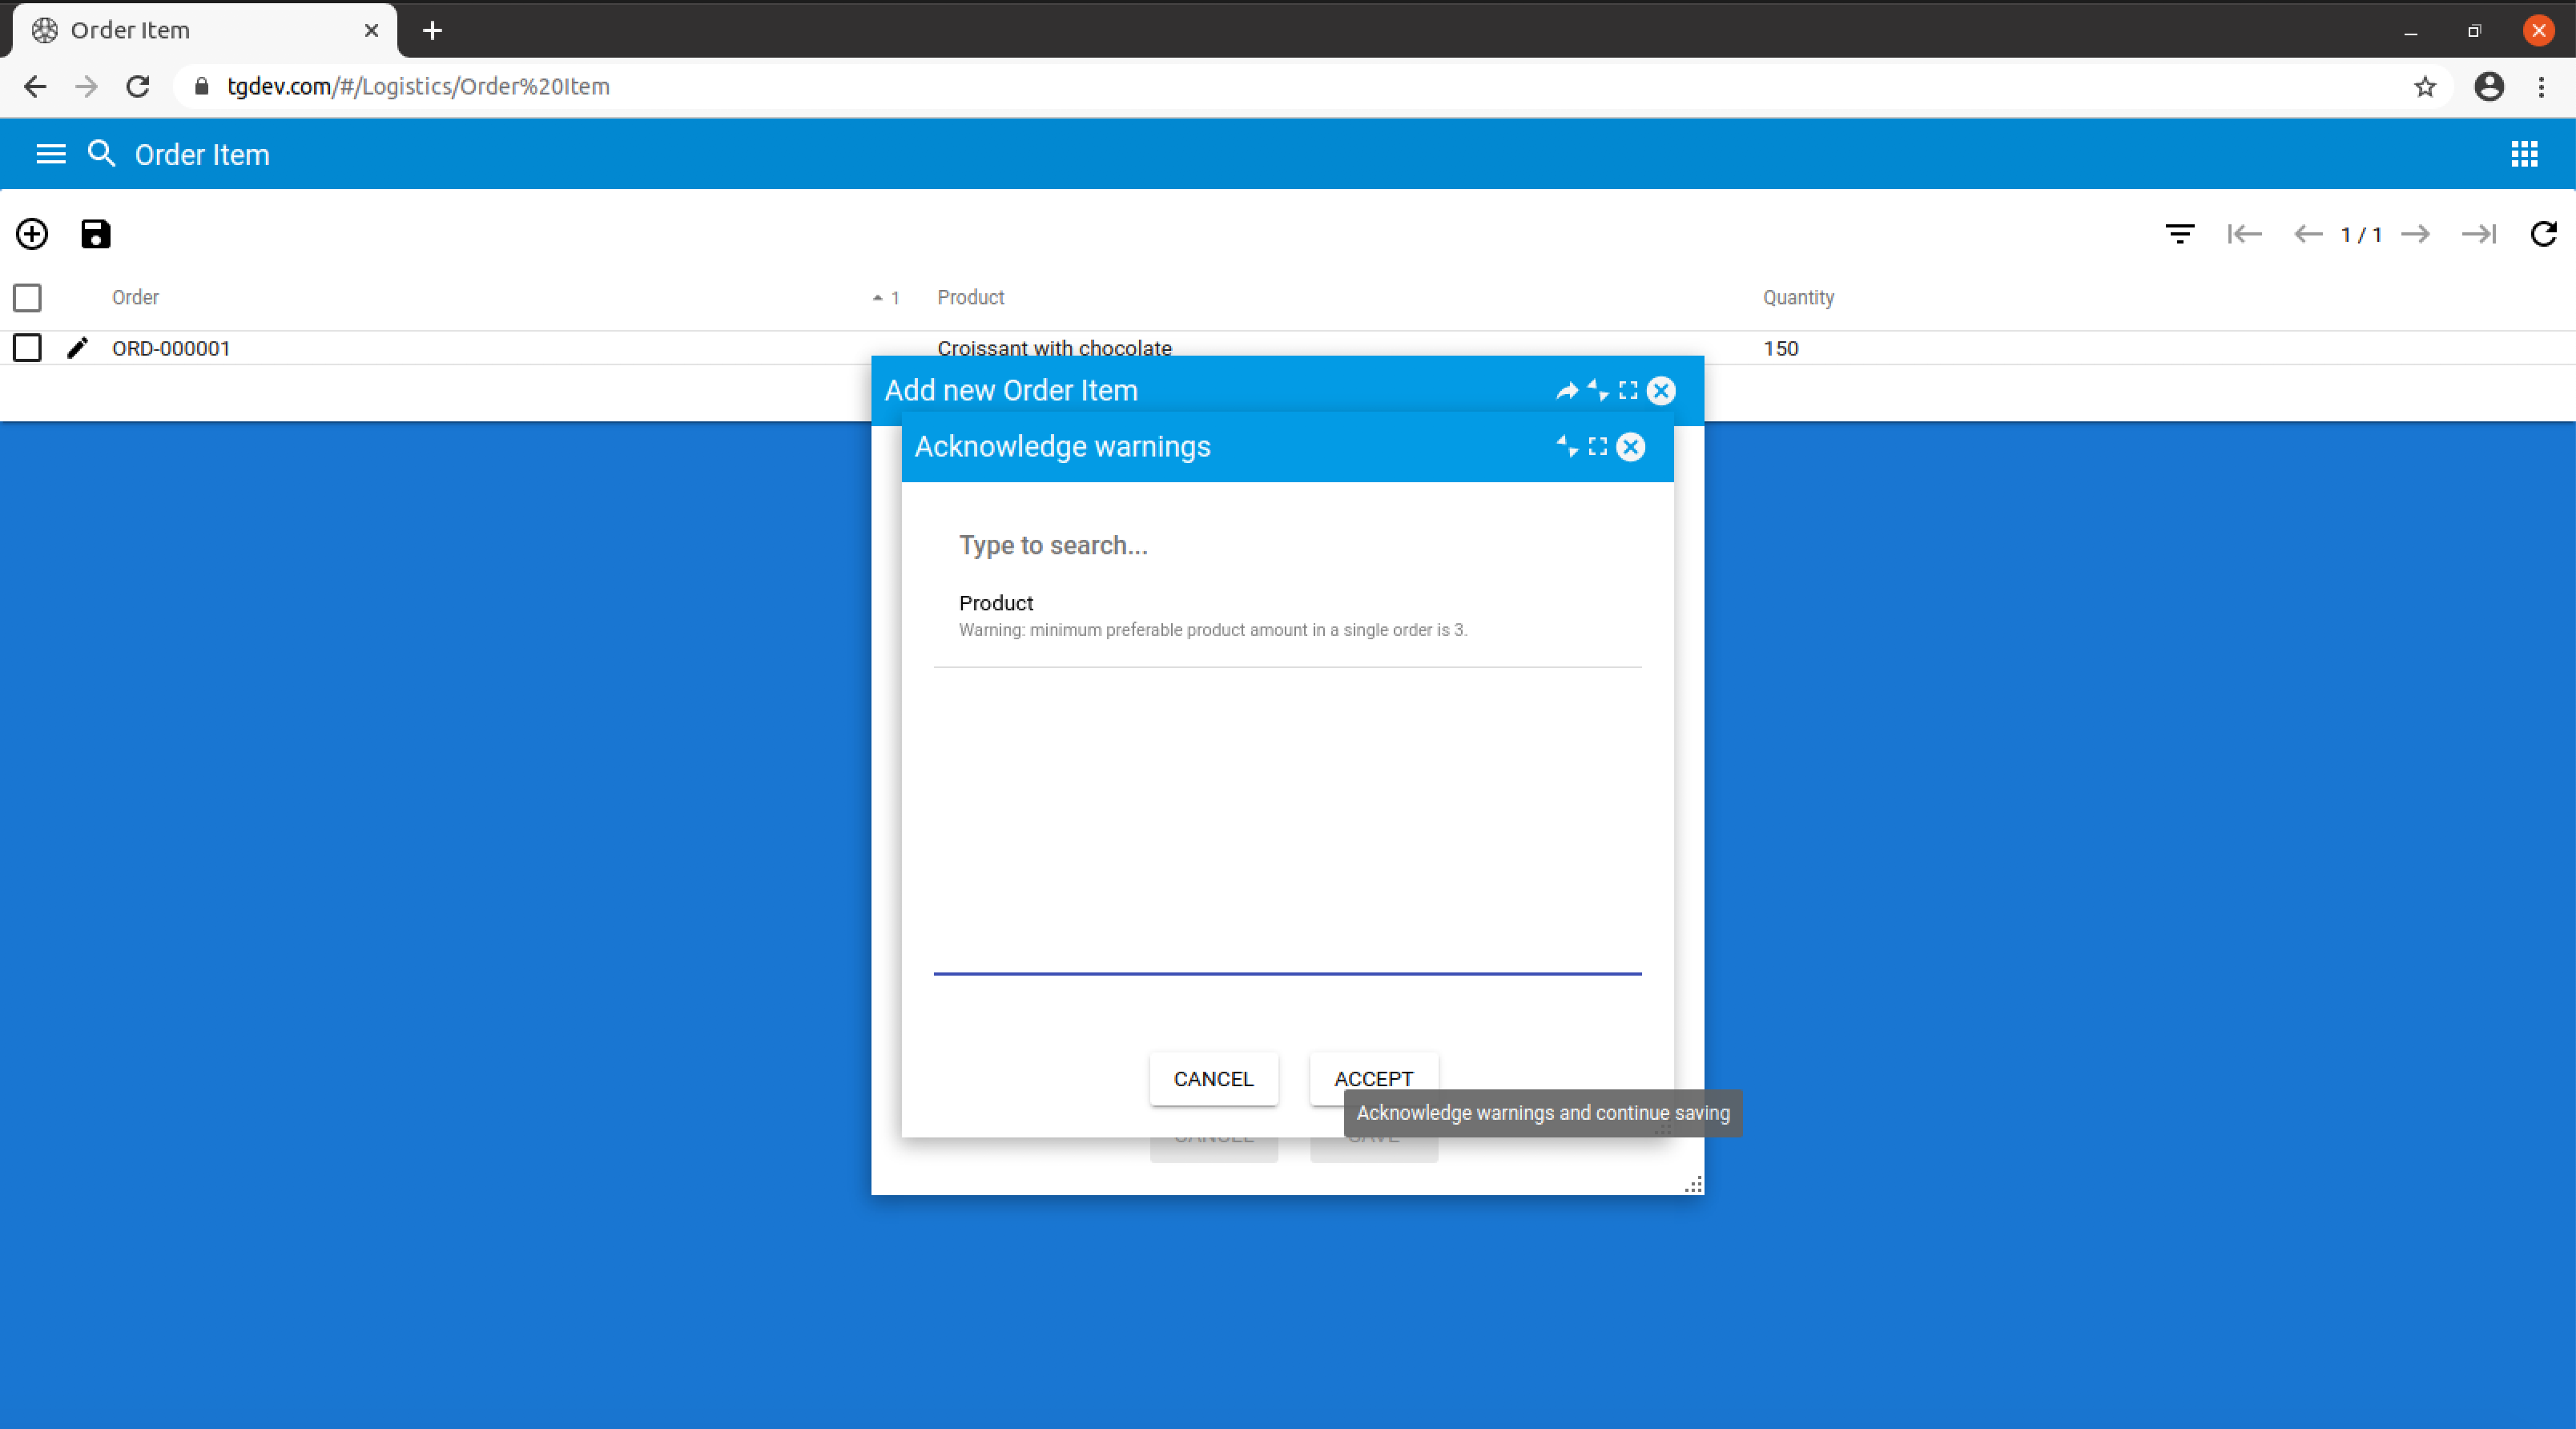
\includegraphics[width=\textwidth]{sections/01-chapter/images/orderitem13.png}


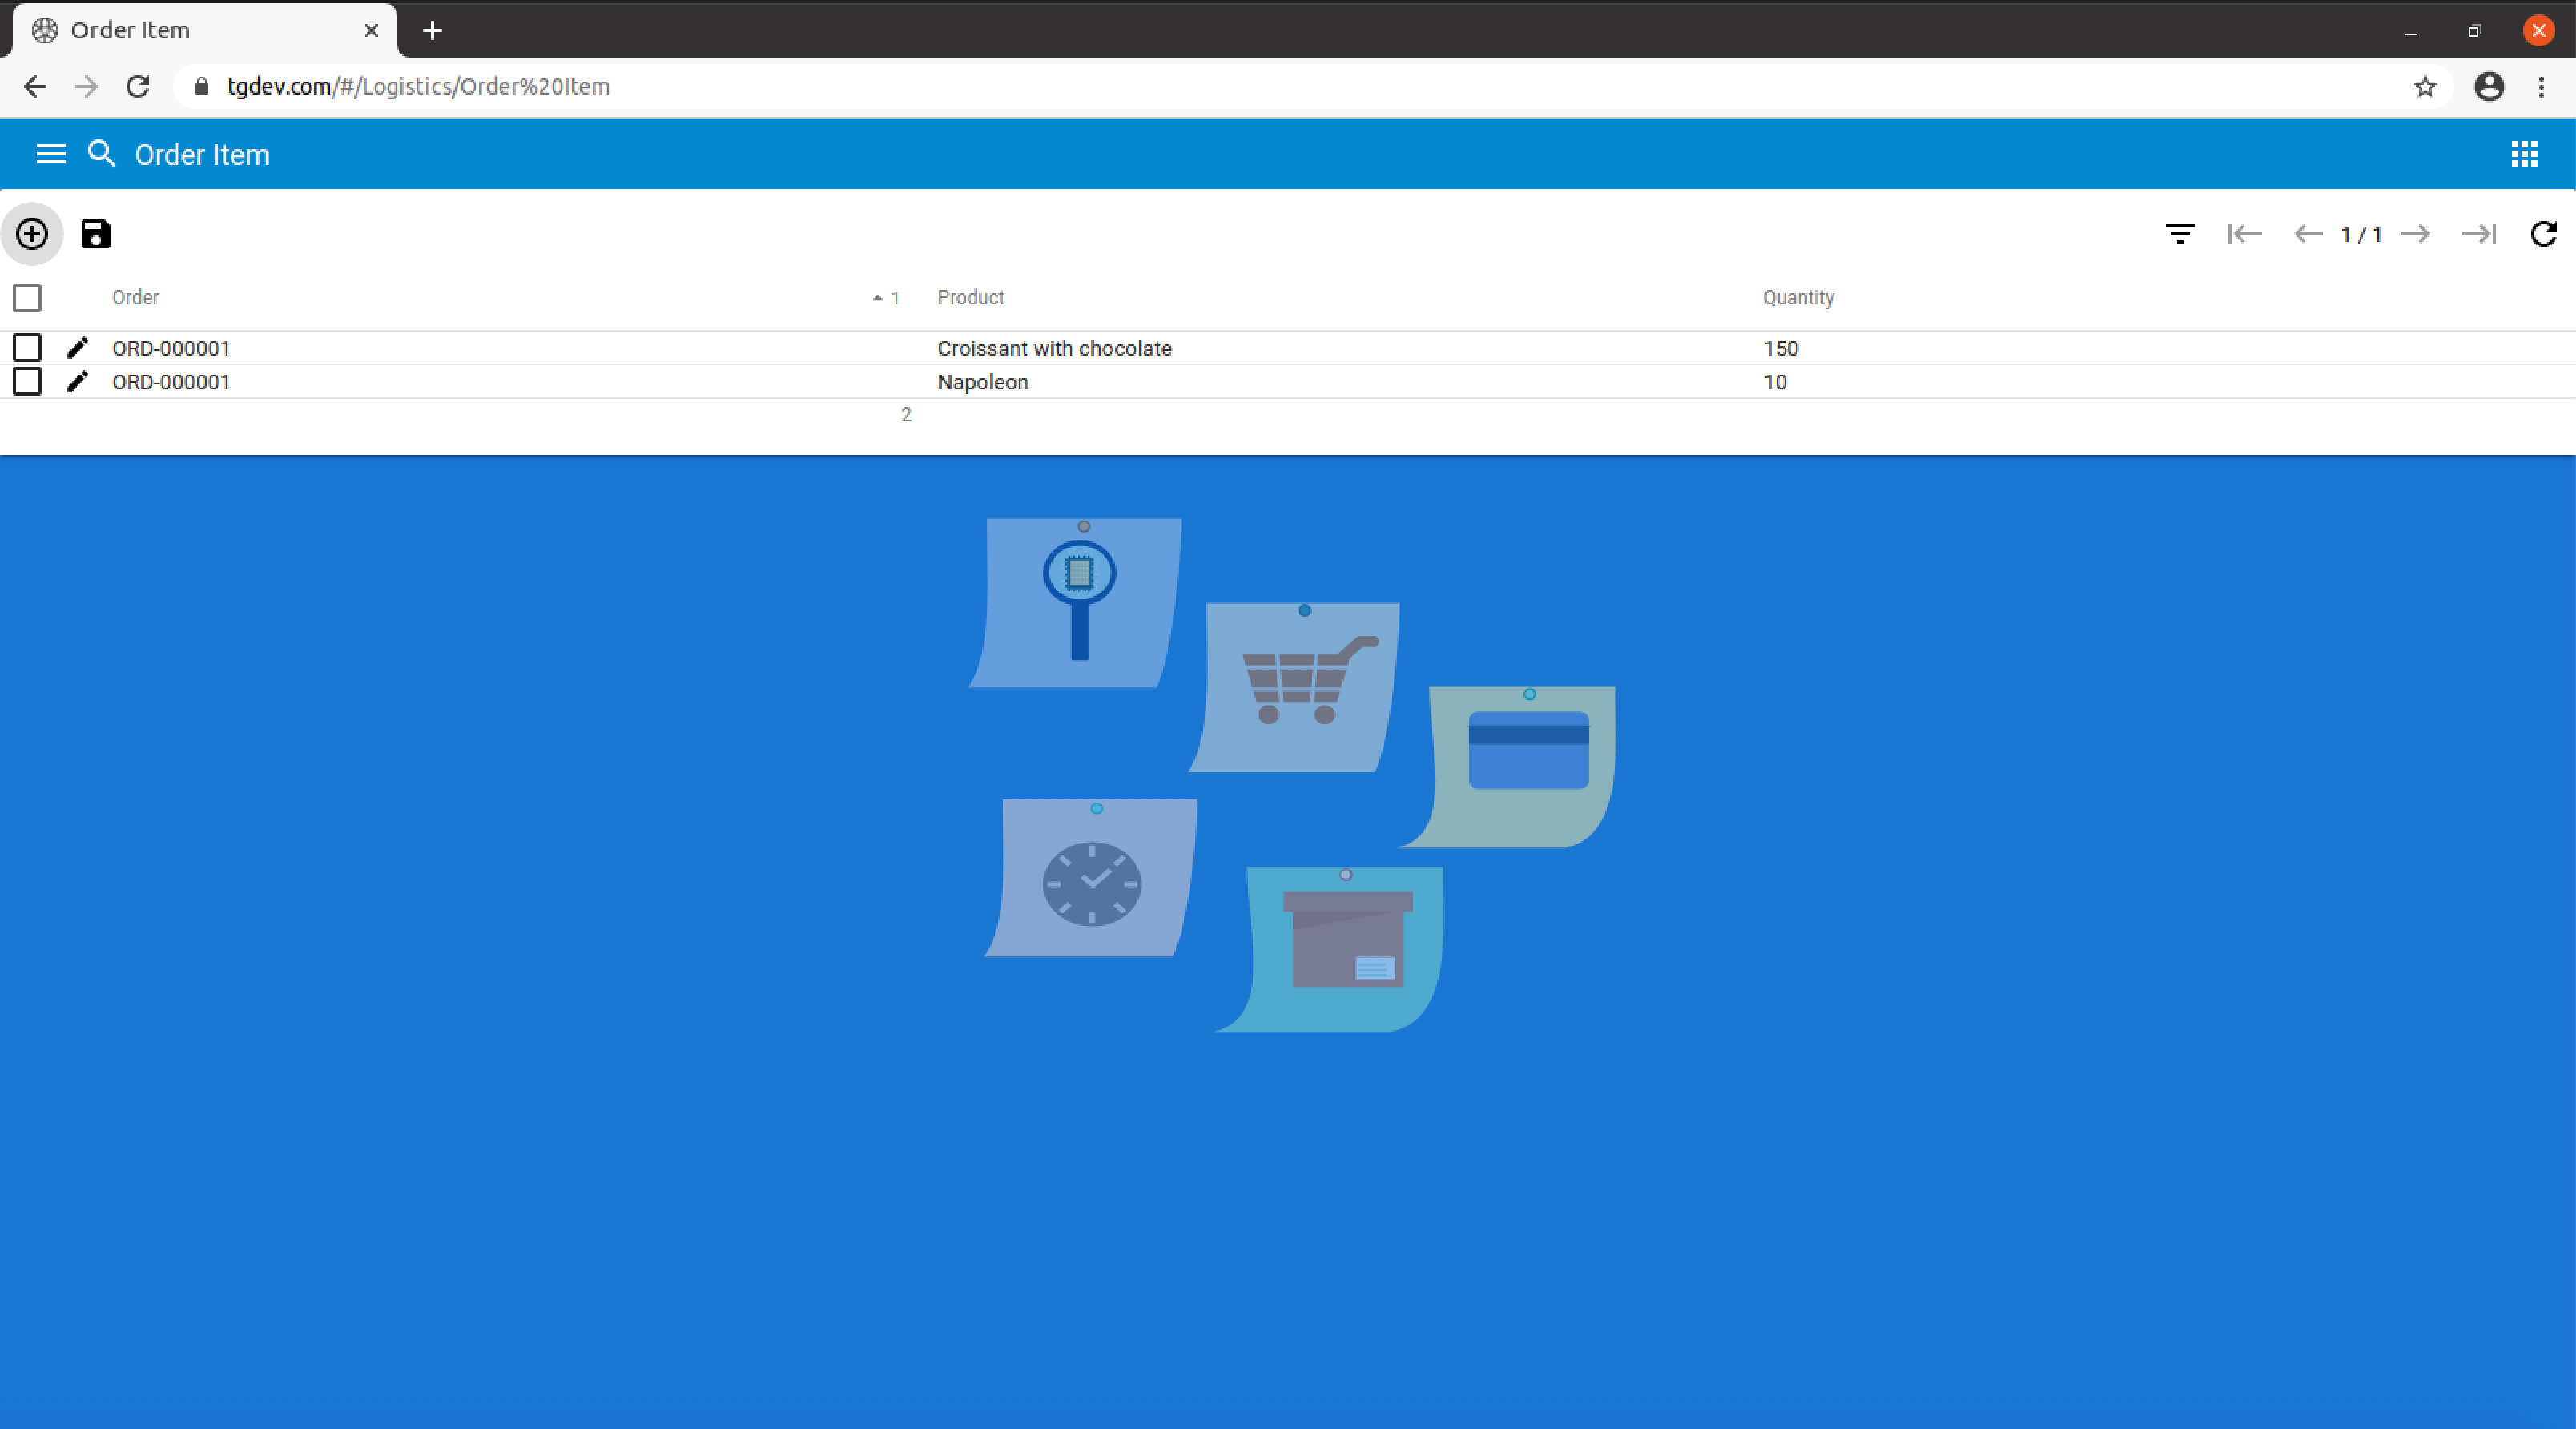
\includegraphics[width=\textwidth]{sections/01-chapter/images/orderitem14.png}


The Warning under the Product informs about a minimum preferable product amount in a single order that is equal 2.One should accept it to proceed.

Some of the restrictions which are important with the OrderItem entity:
No more than 10 products can be added to an order. The least amount of types of products in an order is set to 3. The user is not able to add the same product, if it is already added.

Thus the content of an order can be visible by the search in the OrderItem table using the search criteria → orderNo.


\section{Production}

The Production section consist of the only Entity Product.

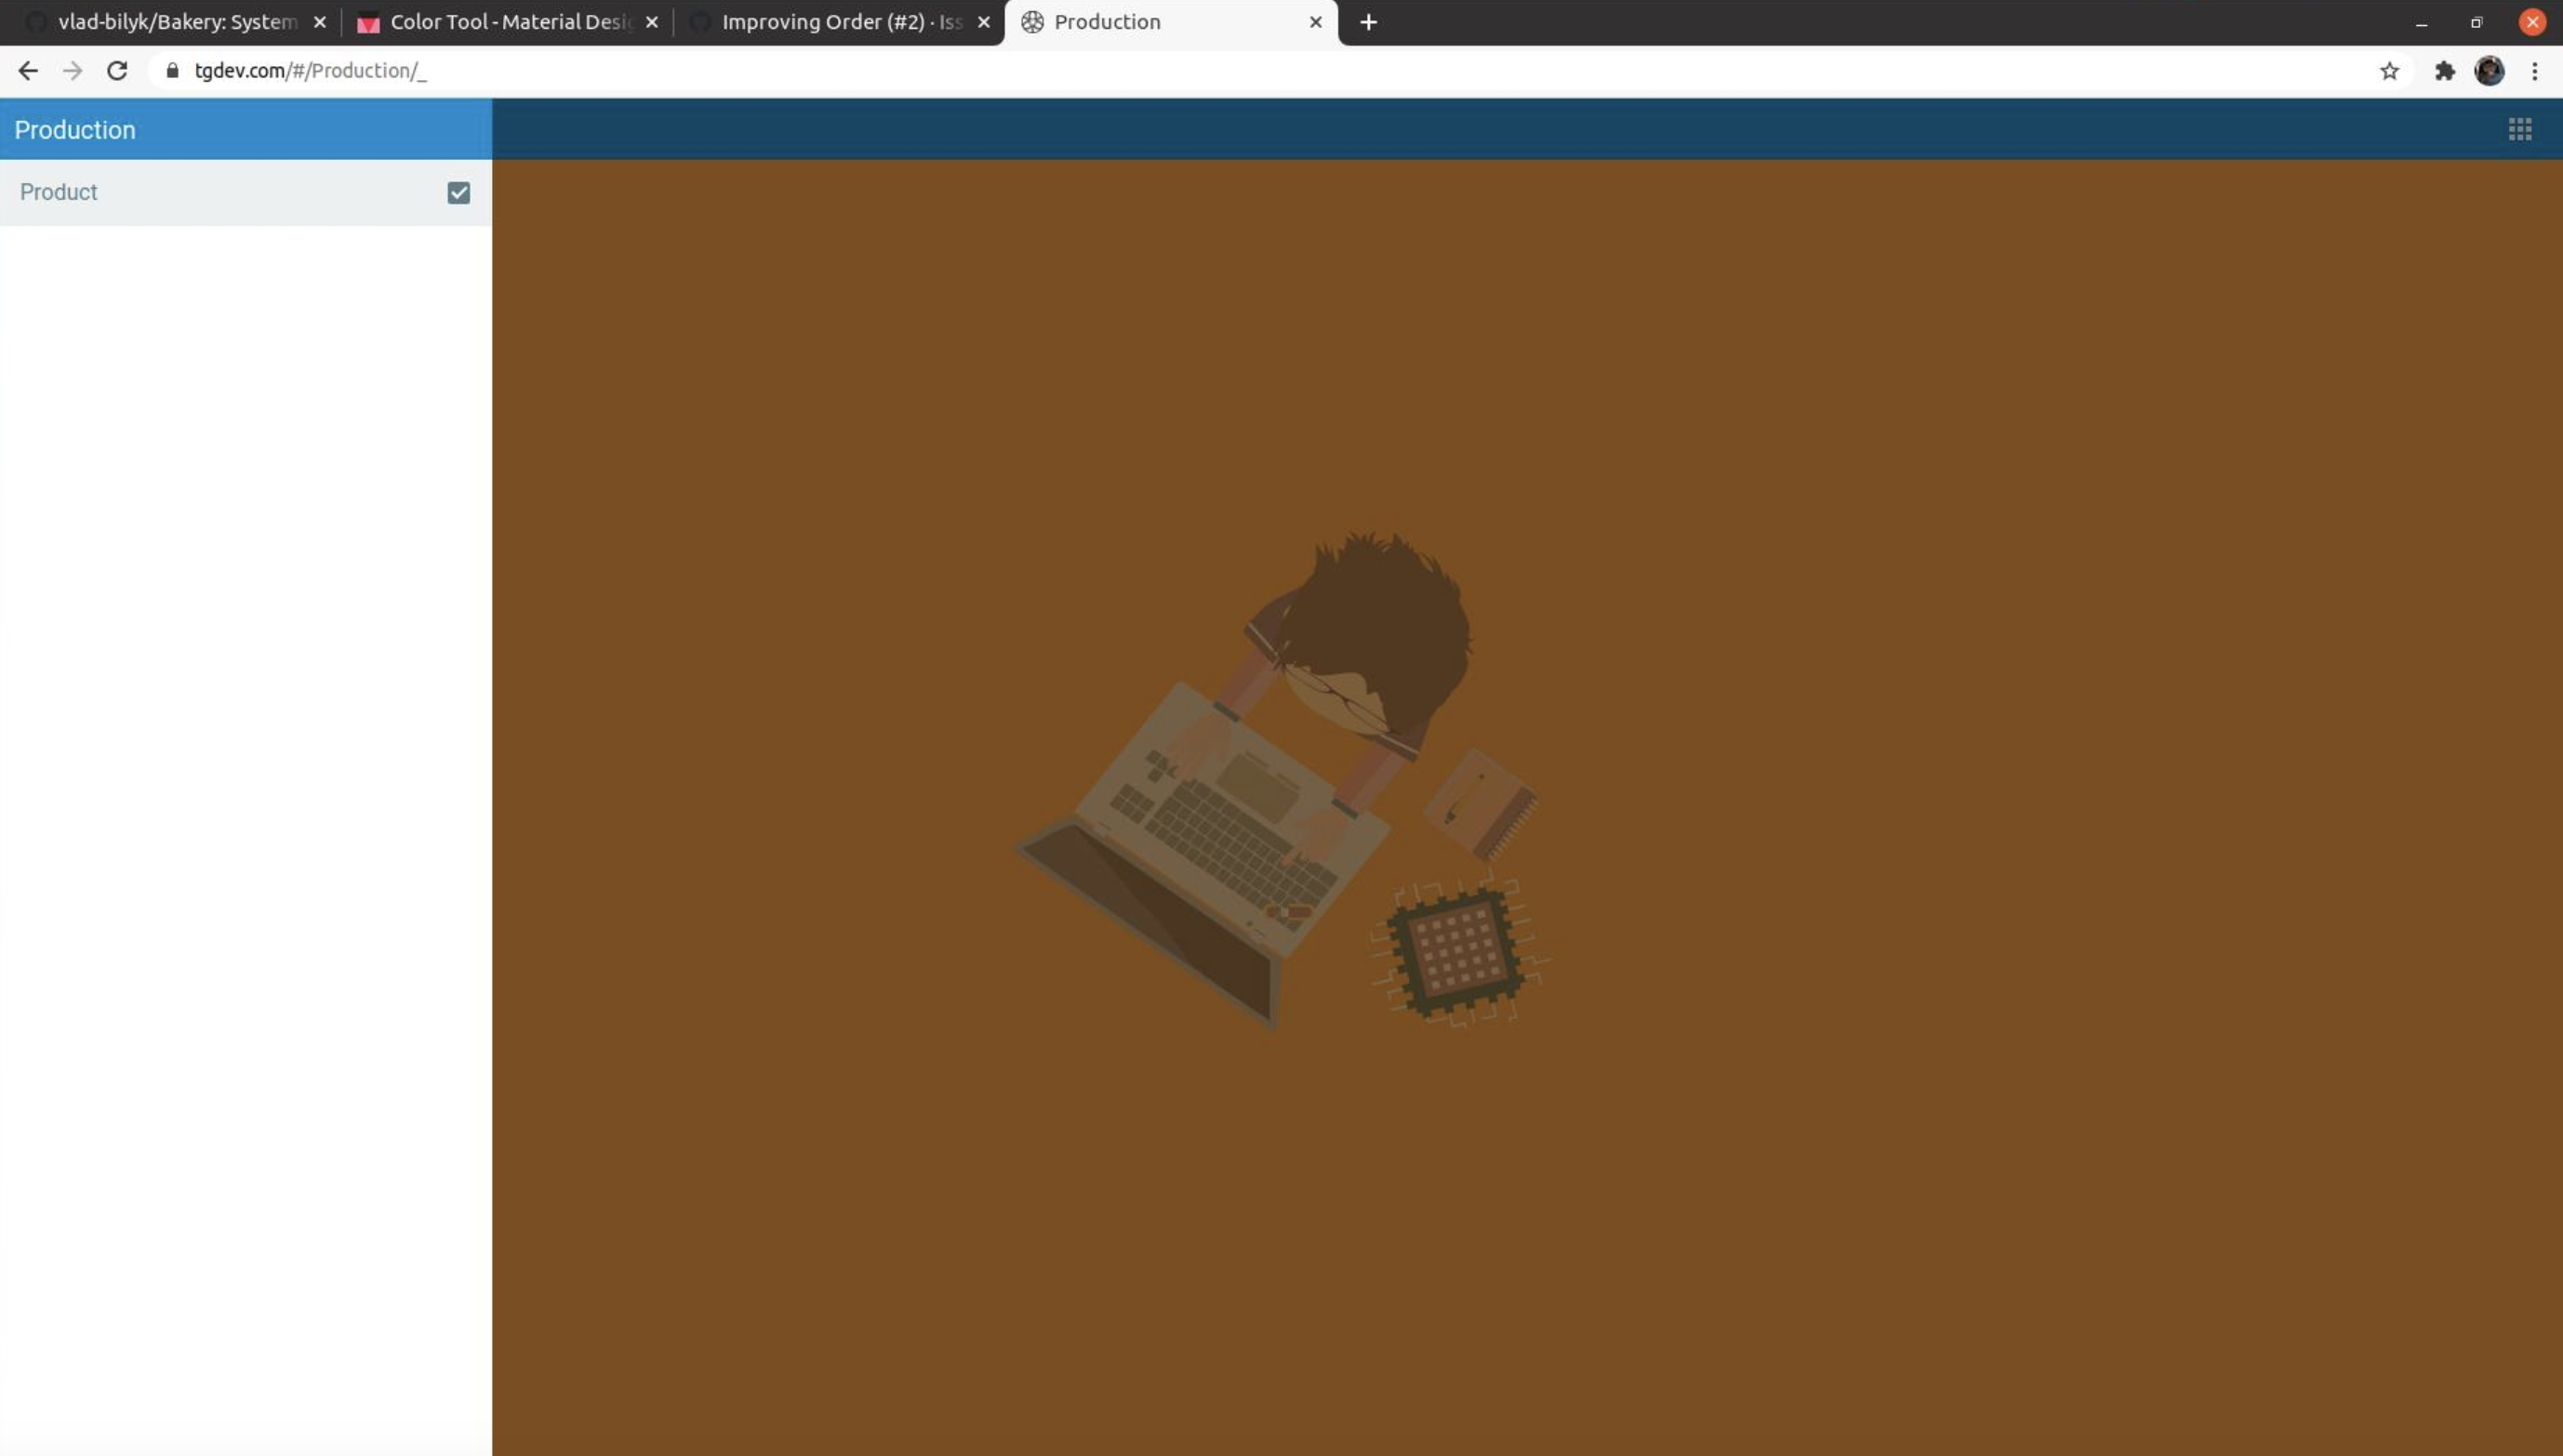
\includegraphics[width=\textwidth]{sections/01-chapter/images/production.png}

\subsection{Product}

Product represents a good which is produced and sold by the bakery.

To search for a Product one can select the following search criteria:

- Product, which is the name of the product

- Description of the product

- Price range of the products

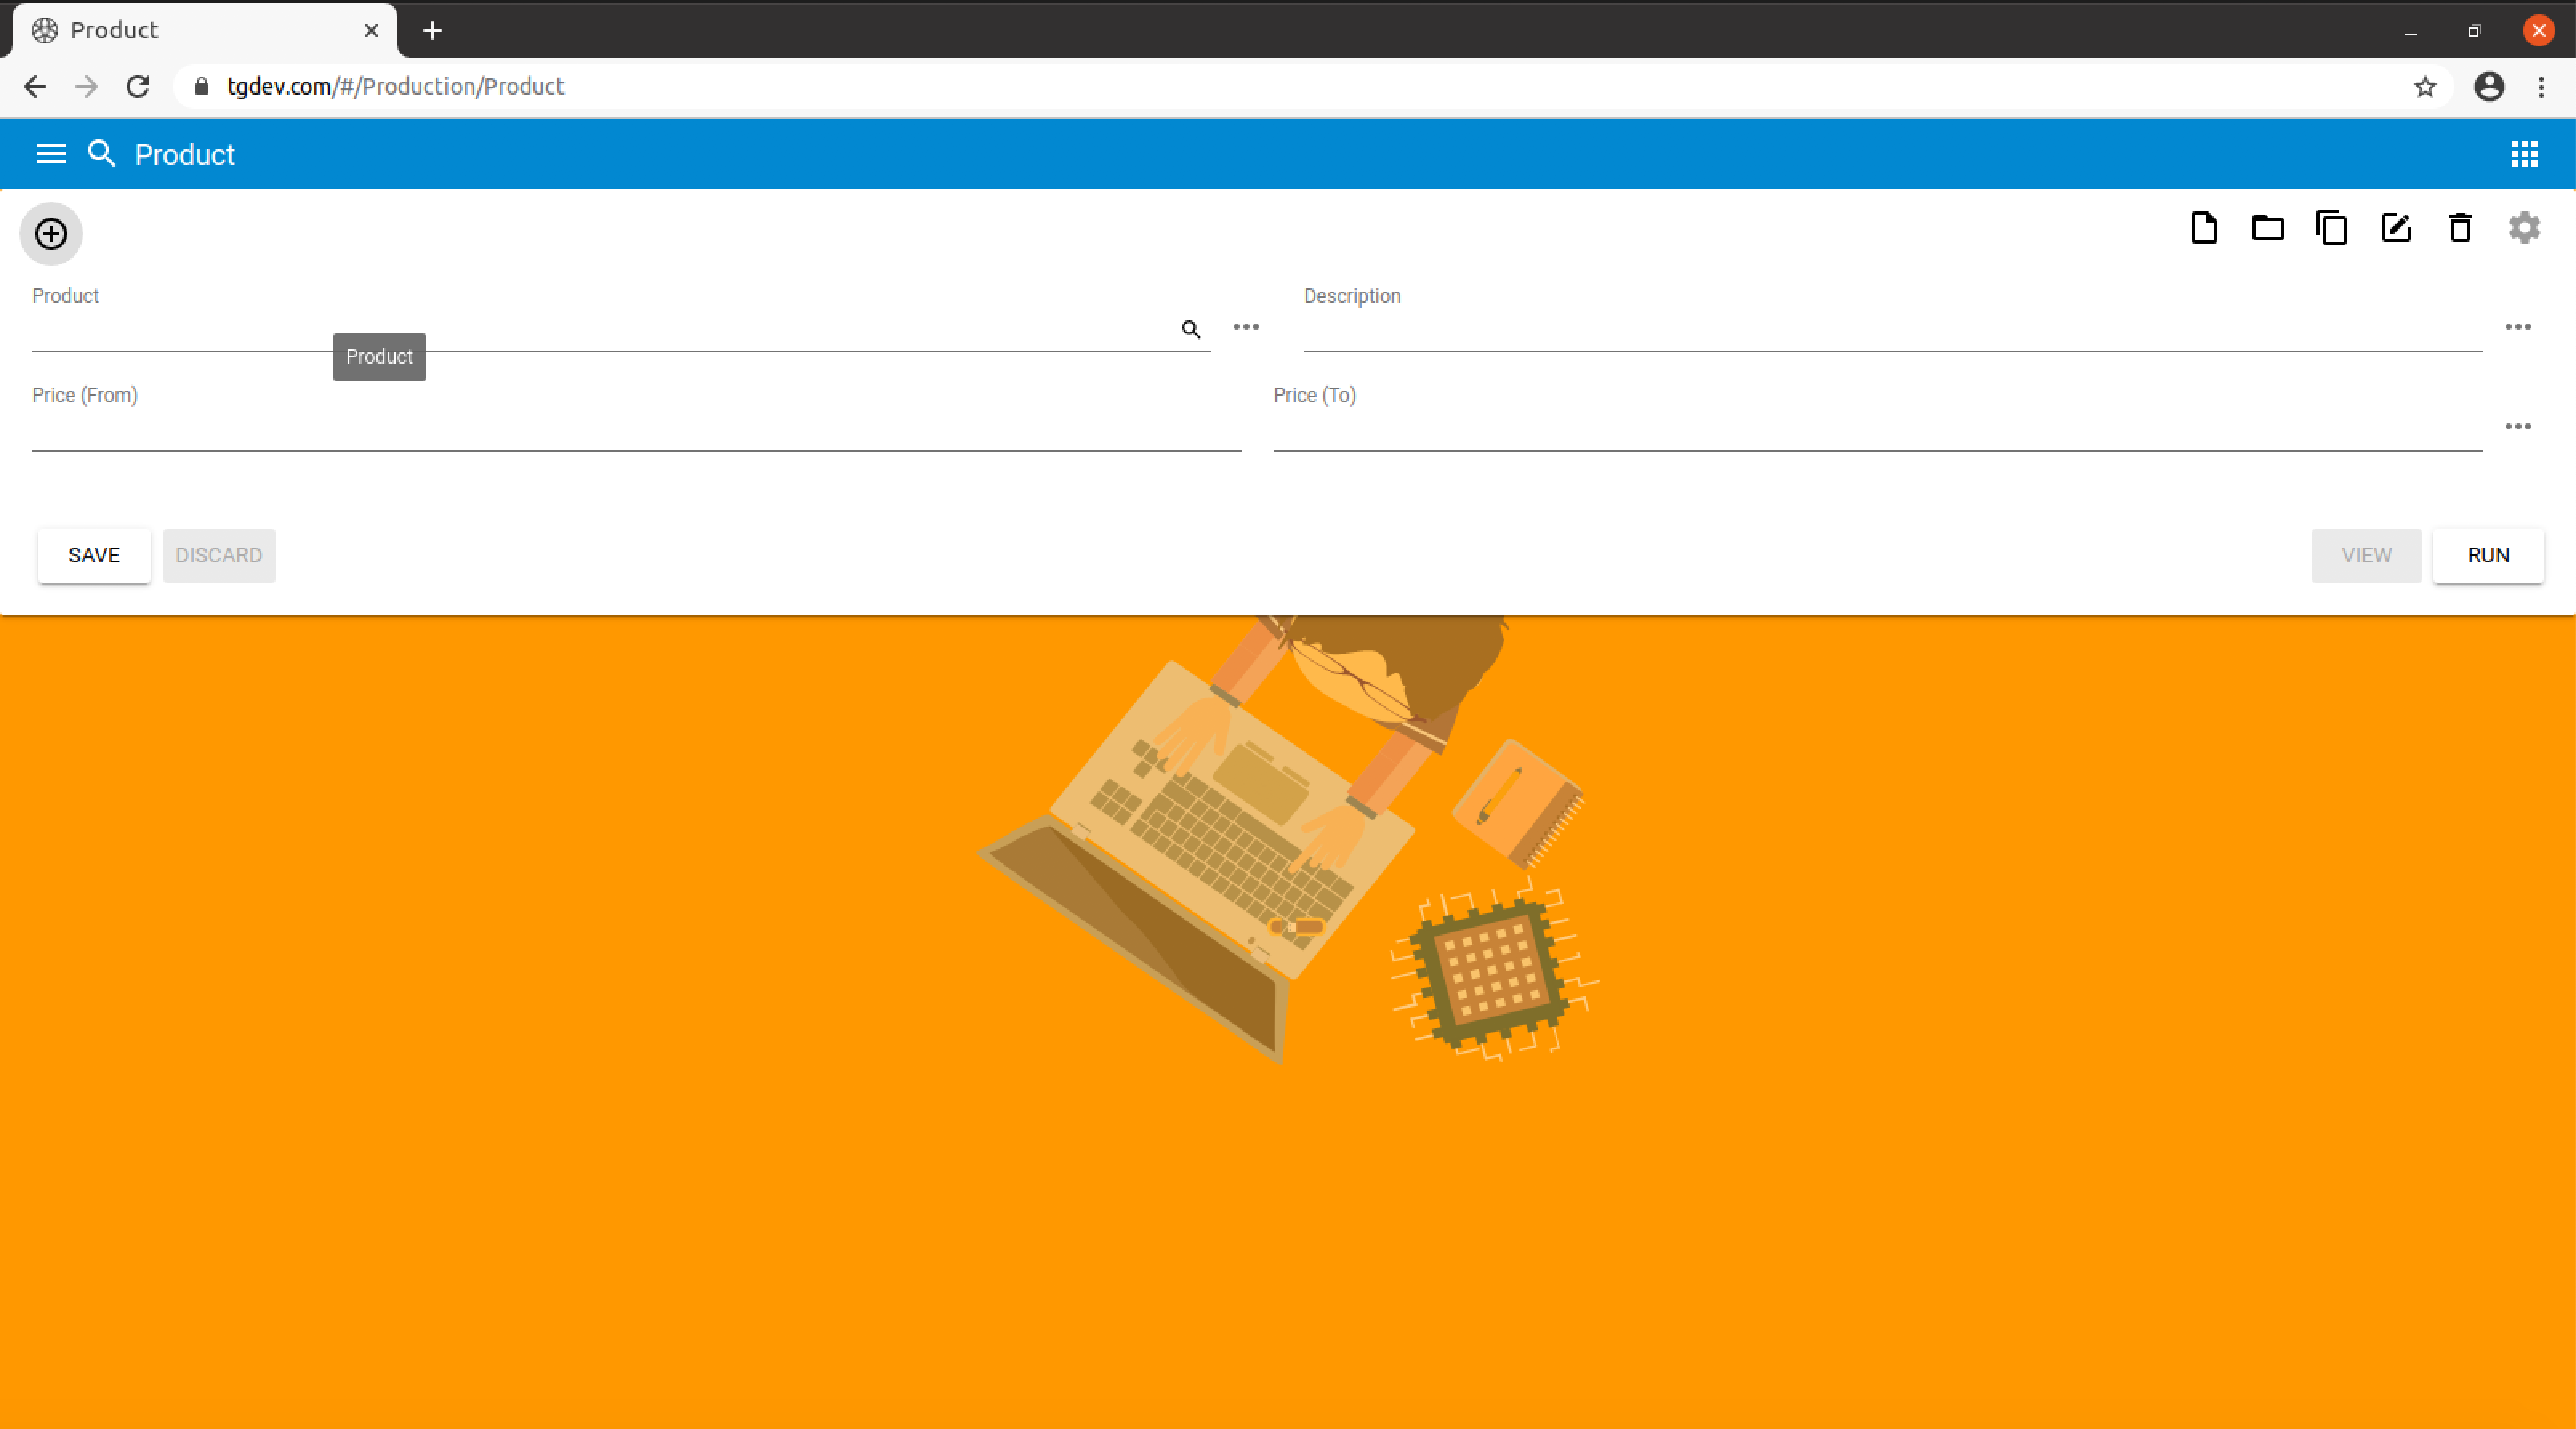
\includegraphics[width=\textwidth]{sections/01-chapter/images/product11.png}

As a system user aka Manager, to register a new product you need to press the plus button and add the product using the following fields:

- Name → required, String, name of the product, cannot contain any numbers.

- Description → optional, String

- Price → required, Money

- Recipe → Optional, String

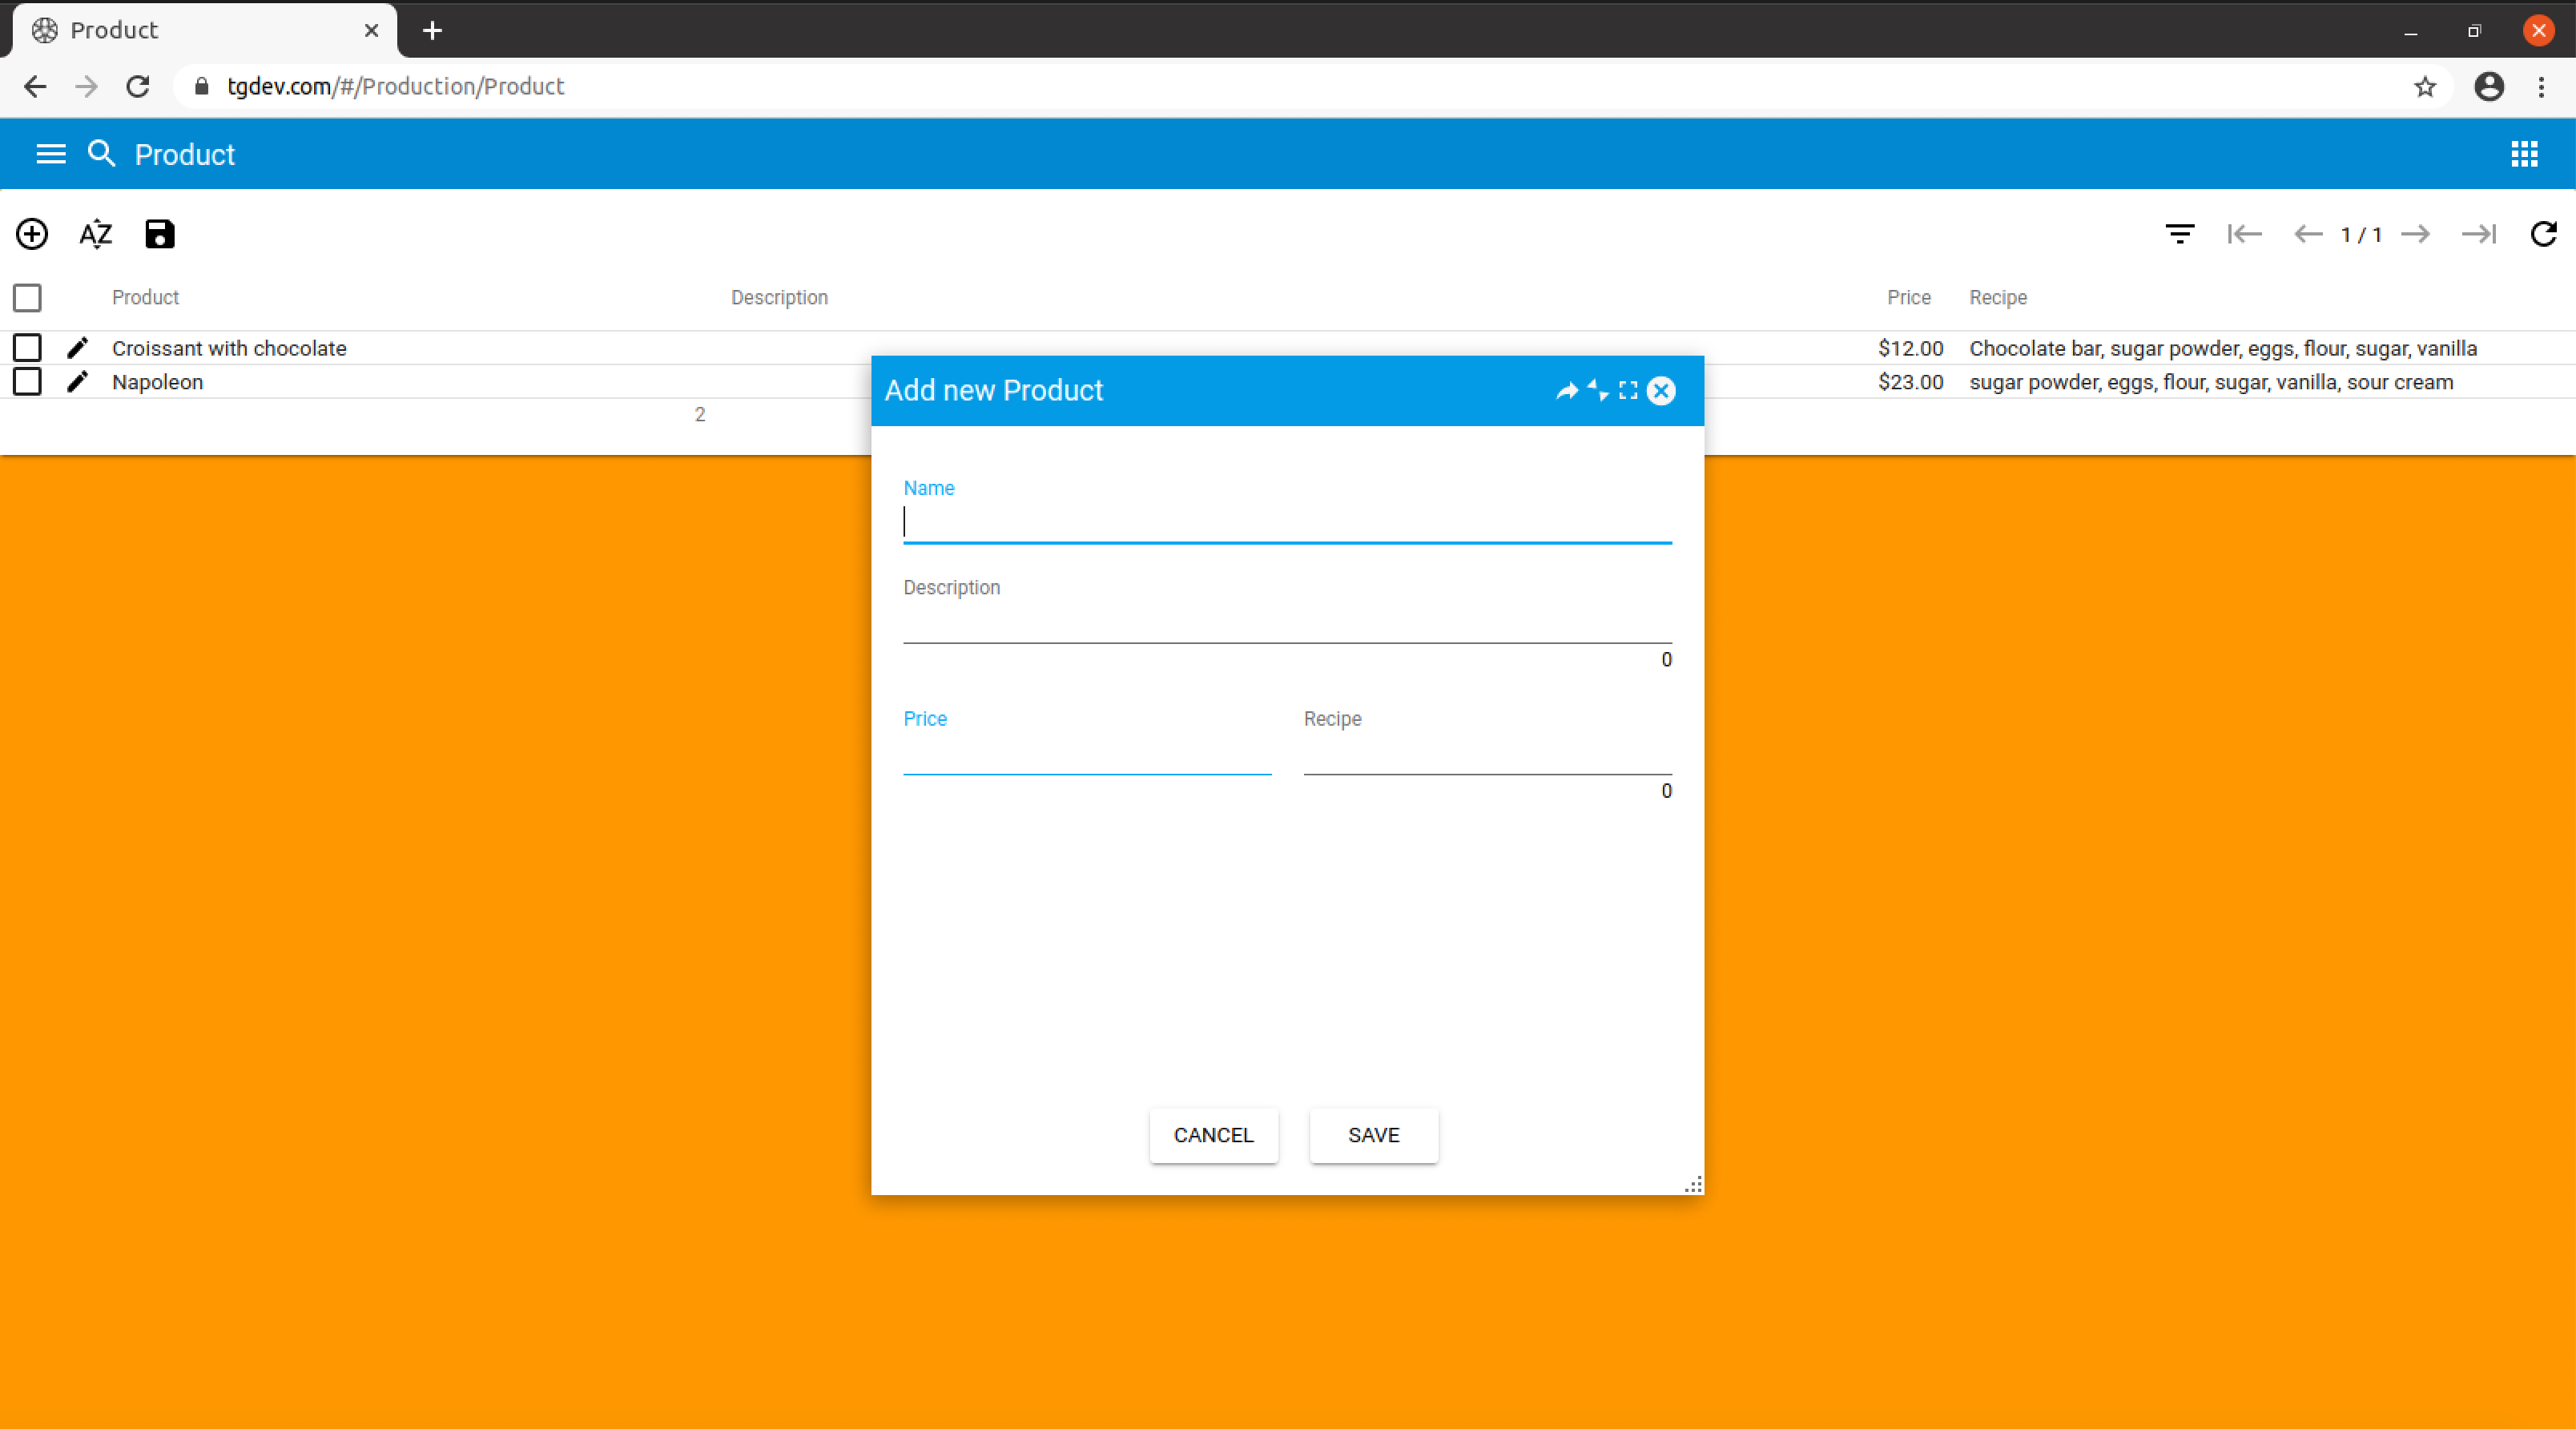
\includegraphics[width=\textwidth]{sections/01-chapter/images/product12.png}

\section{System Users field}

The field System Users describes the System in terms of Roles. 

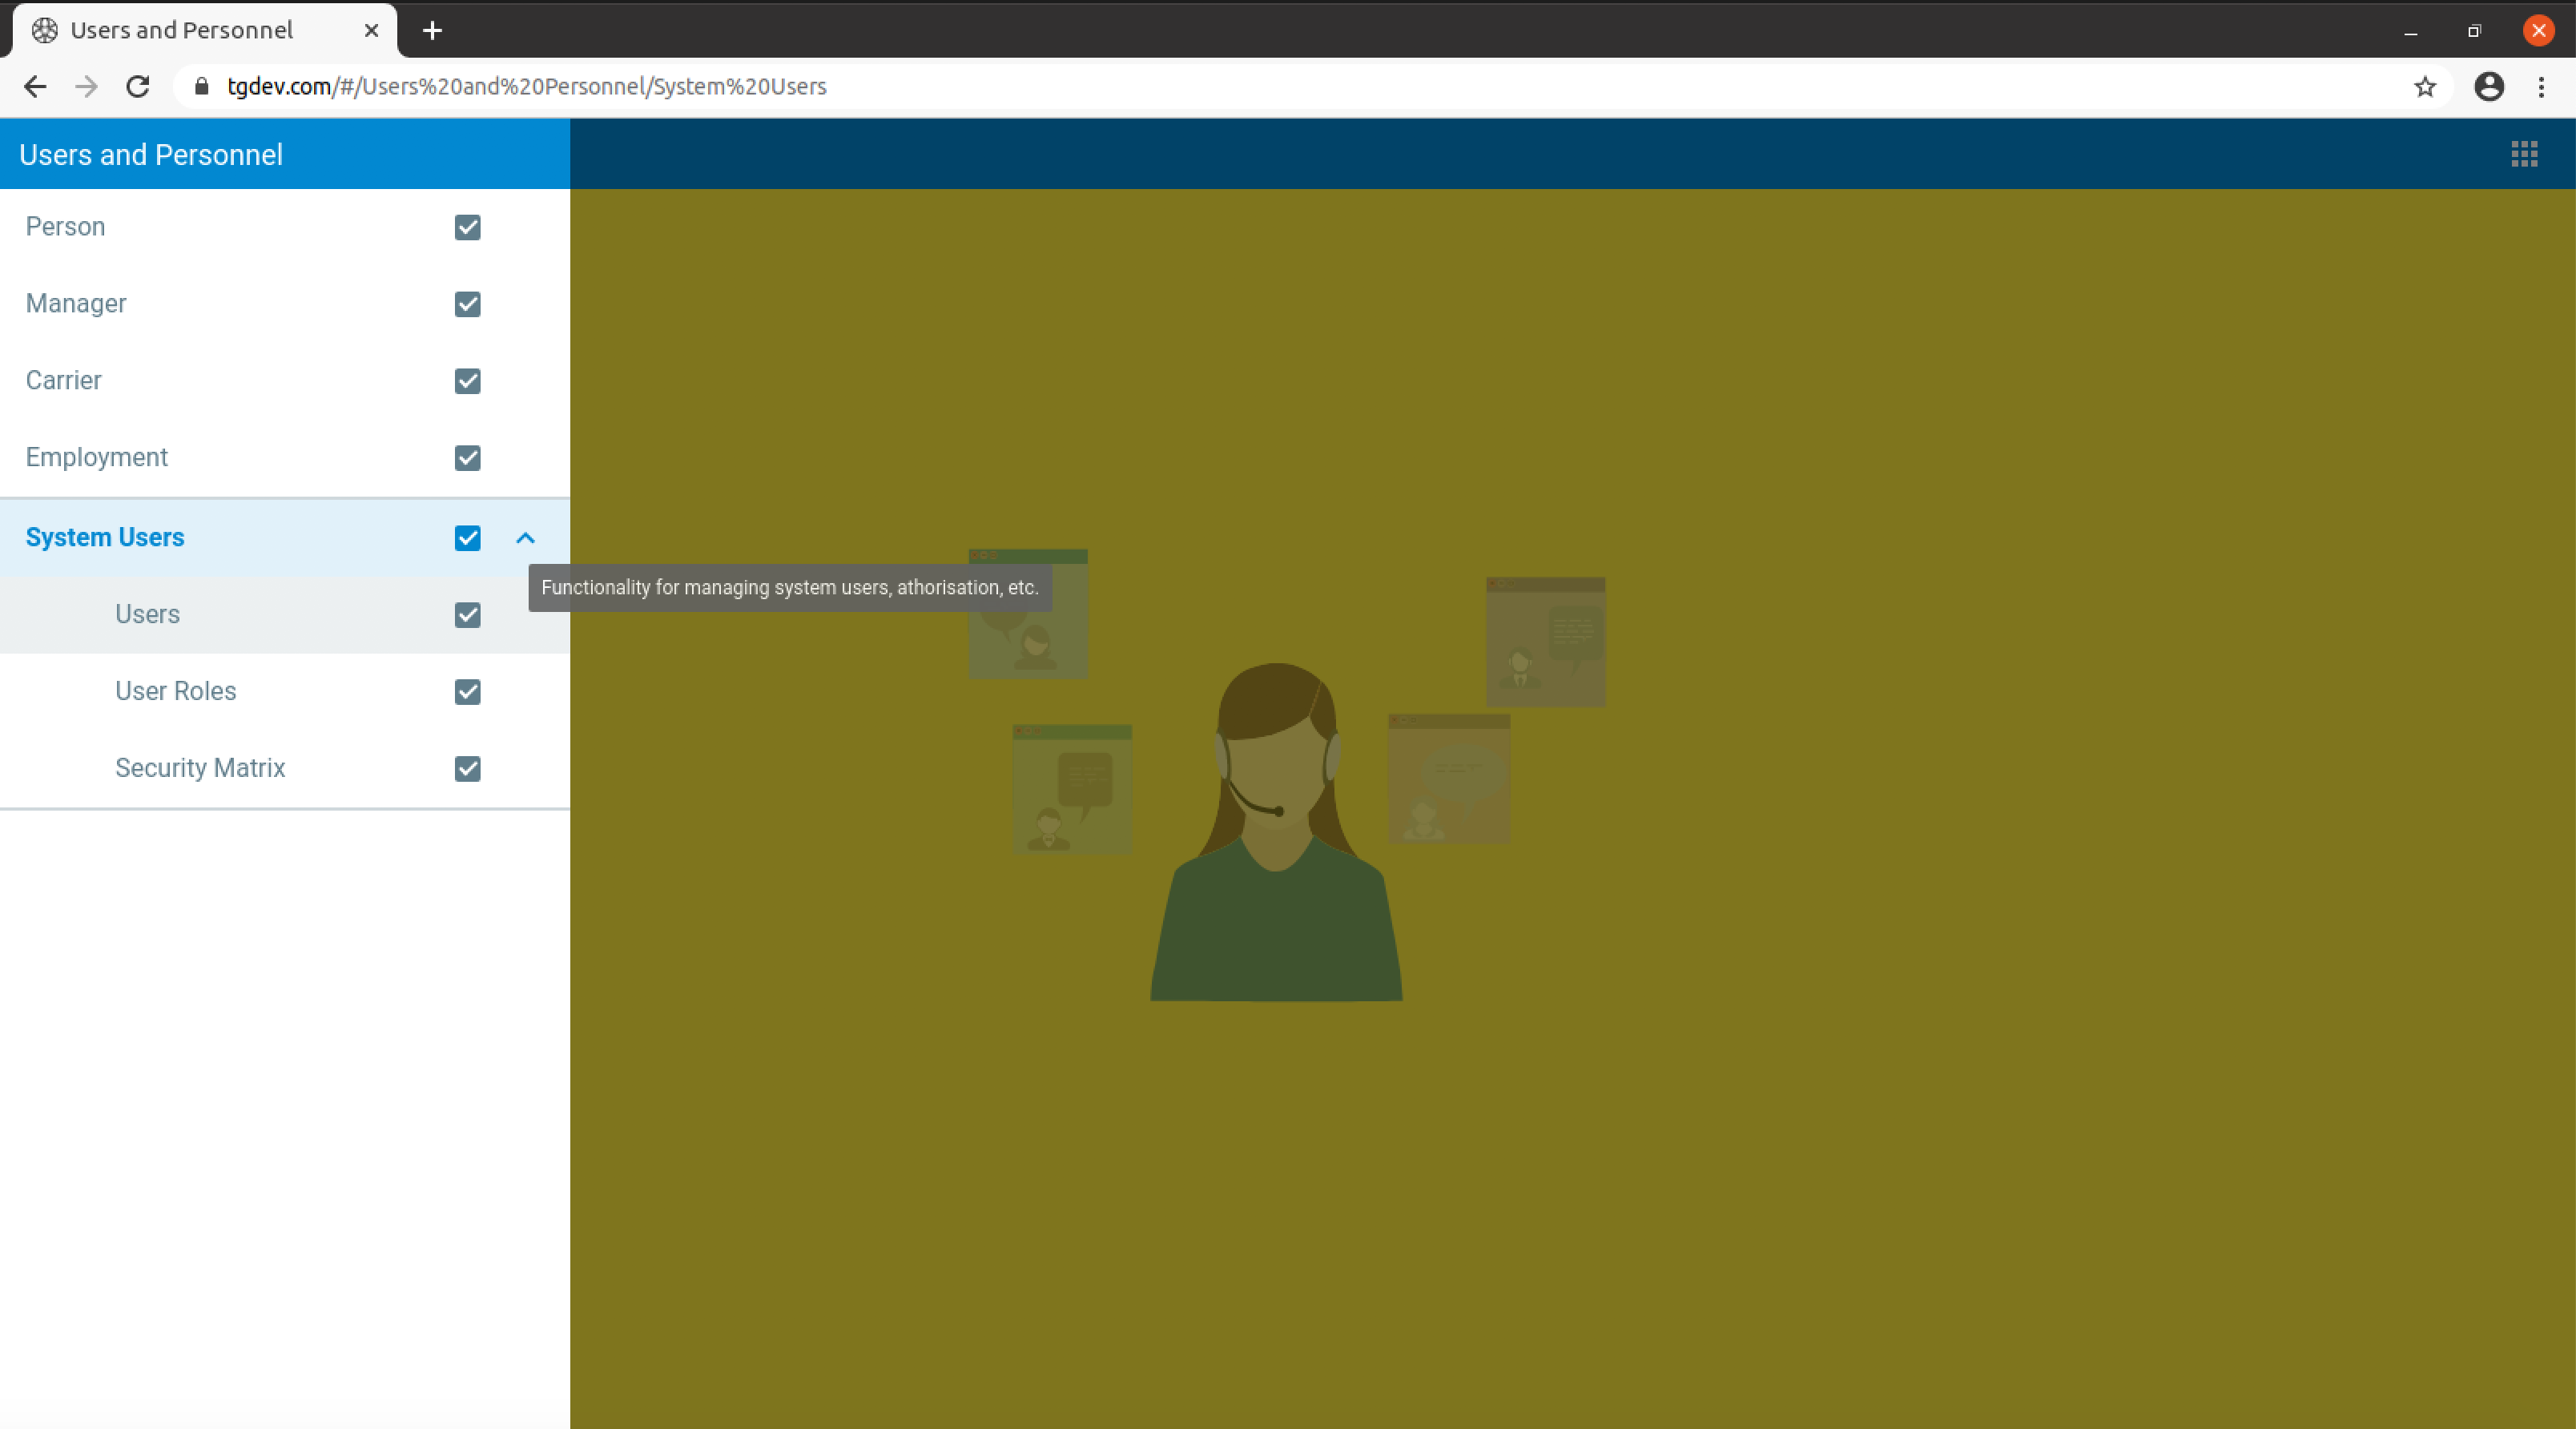
\includegraphics[width=\textwidth]{sections/01-chapter/images/system11.png}

The Entity Users displays all the relevant information about the users present in the system.

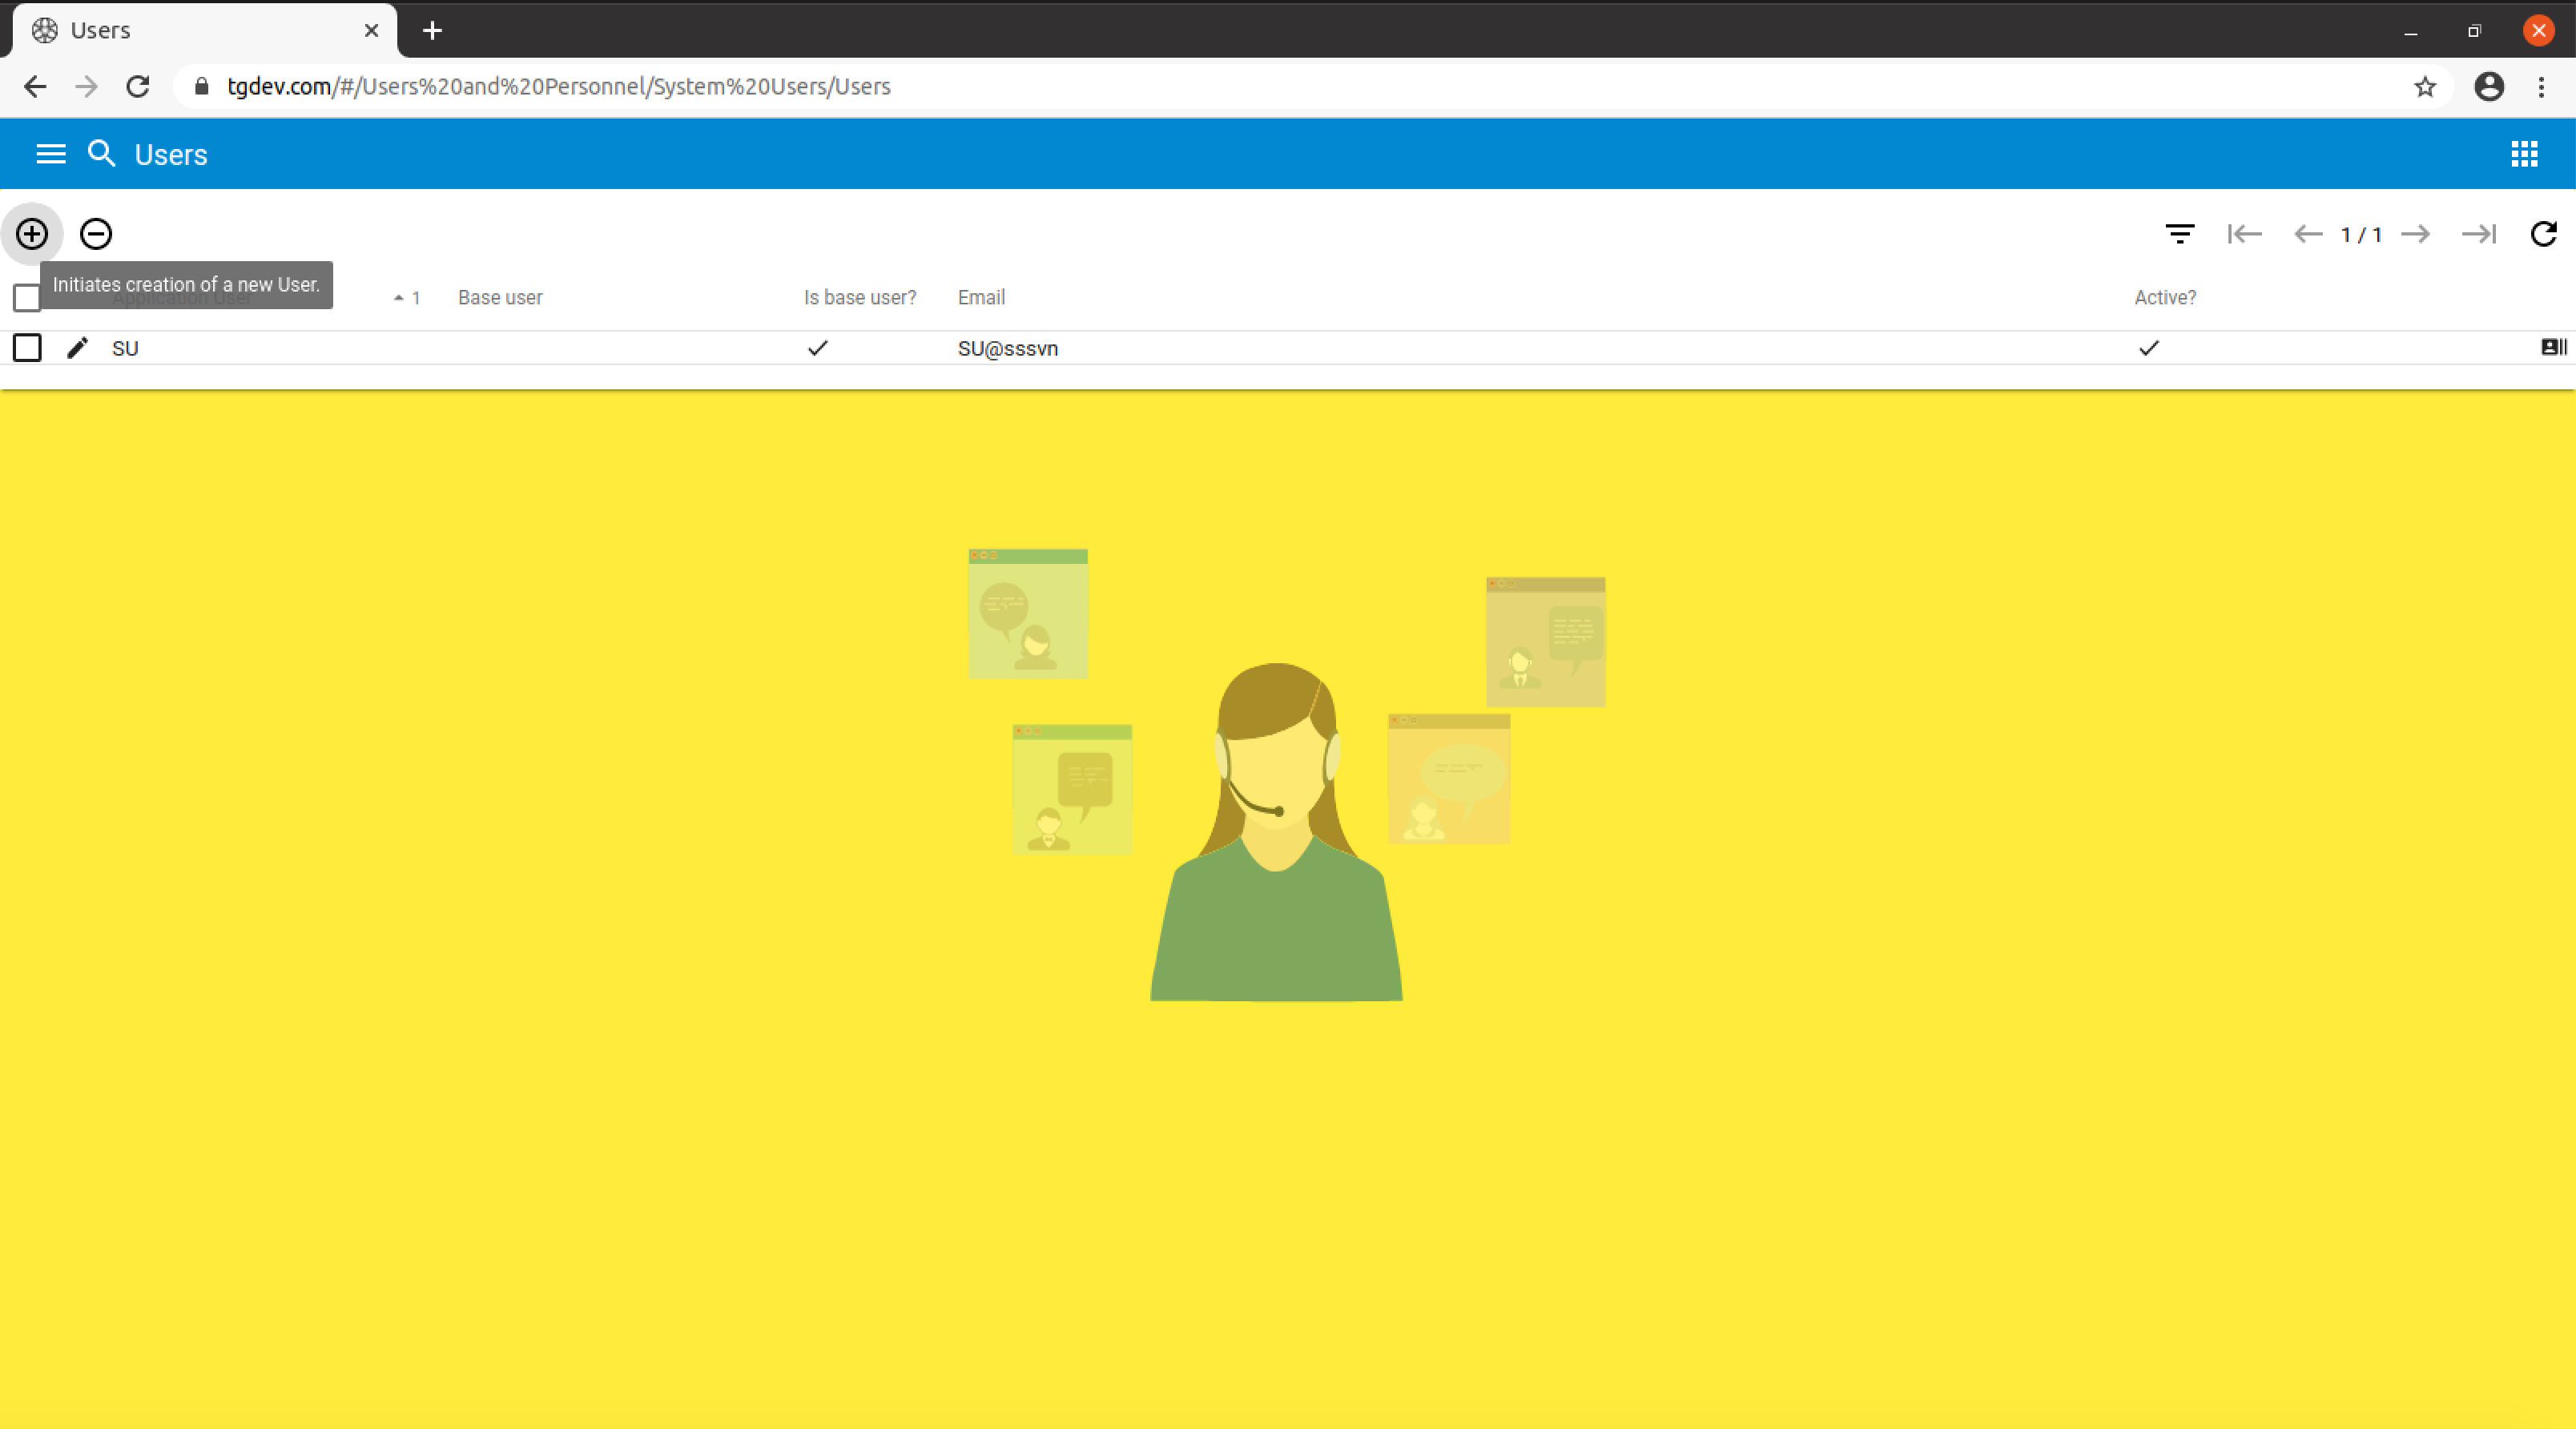
\includegraphics[width=\textwidth]{sections/01-chapter/images/system12.png}

There are multiple roles a User can have in a System. The roles can be created manually. The roles can have different access to data as well as to what one can do within a System.

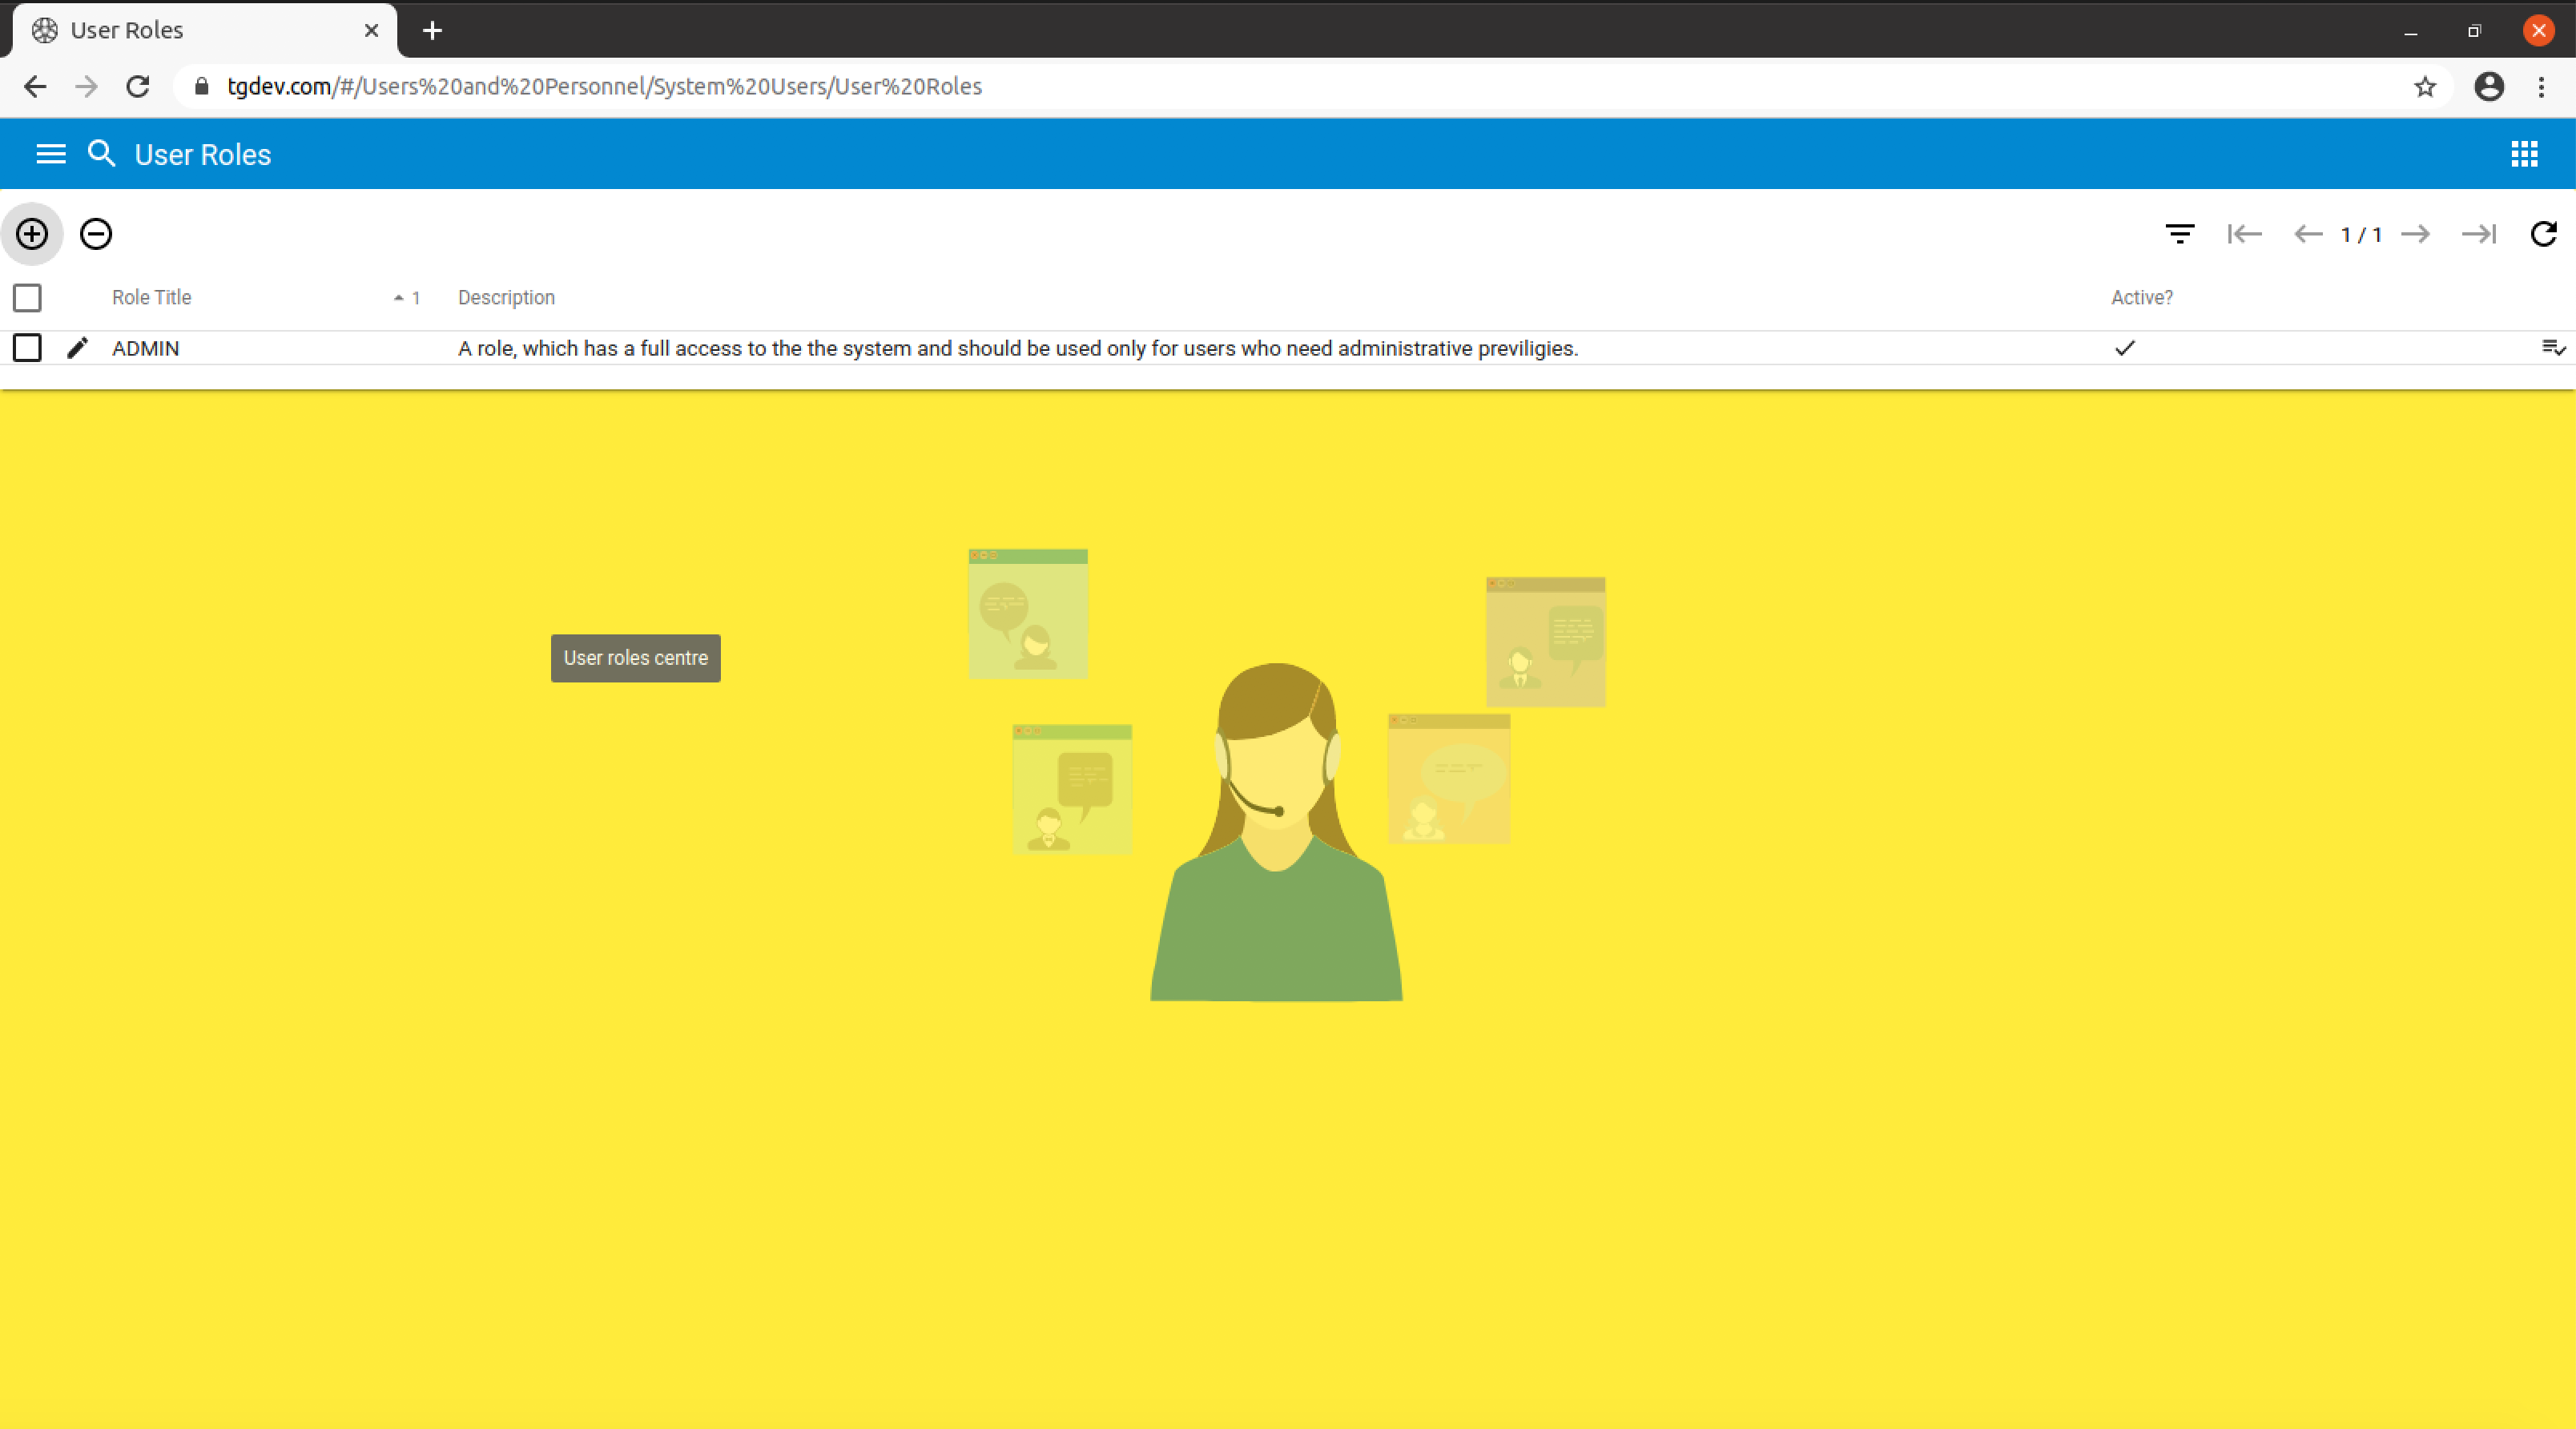
\includegraphics[width=\textwidth]{sections/01-chapter/images/system13.png}

The creation of a new role requires the filling of the information about Role Title as well as description. In order for a system to be able to interact with the set Role the Active option should be turned on.


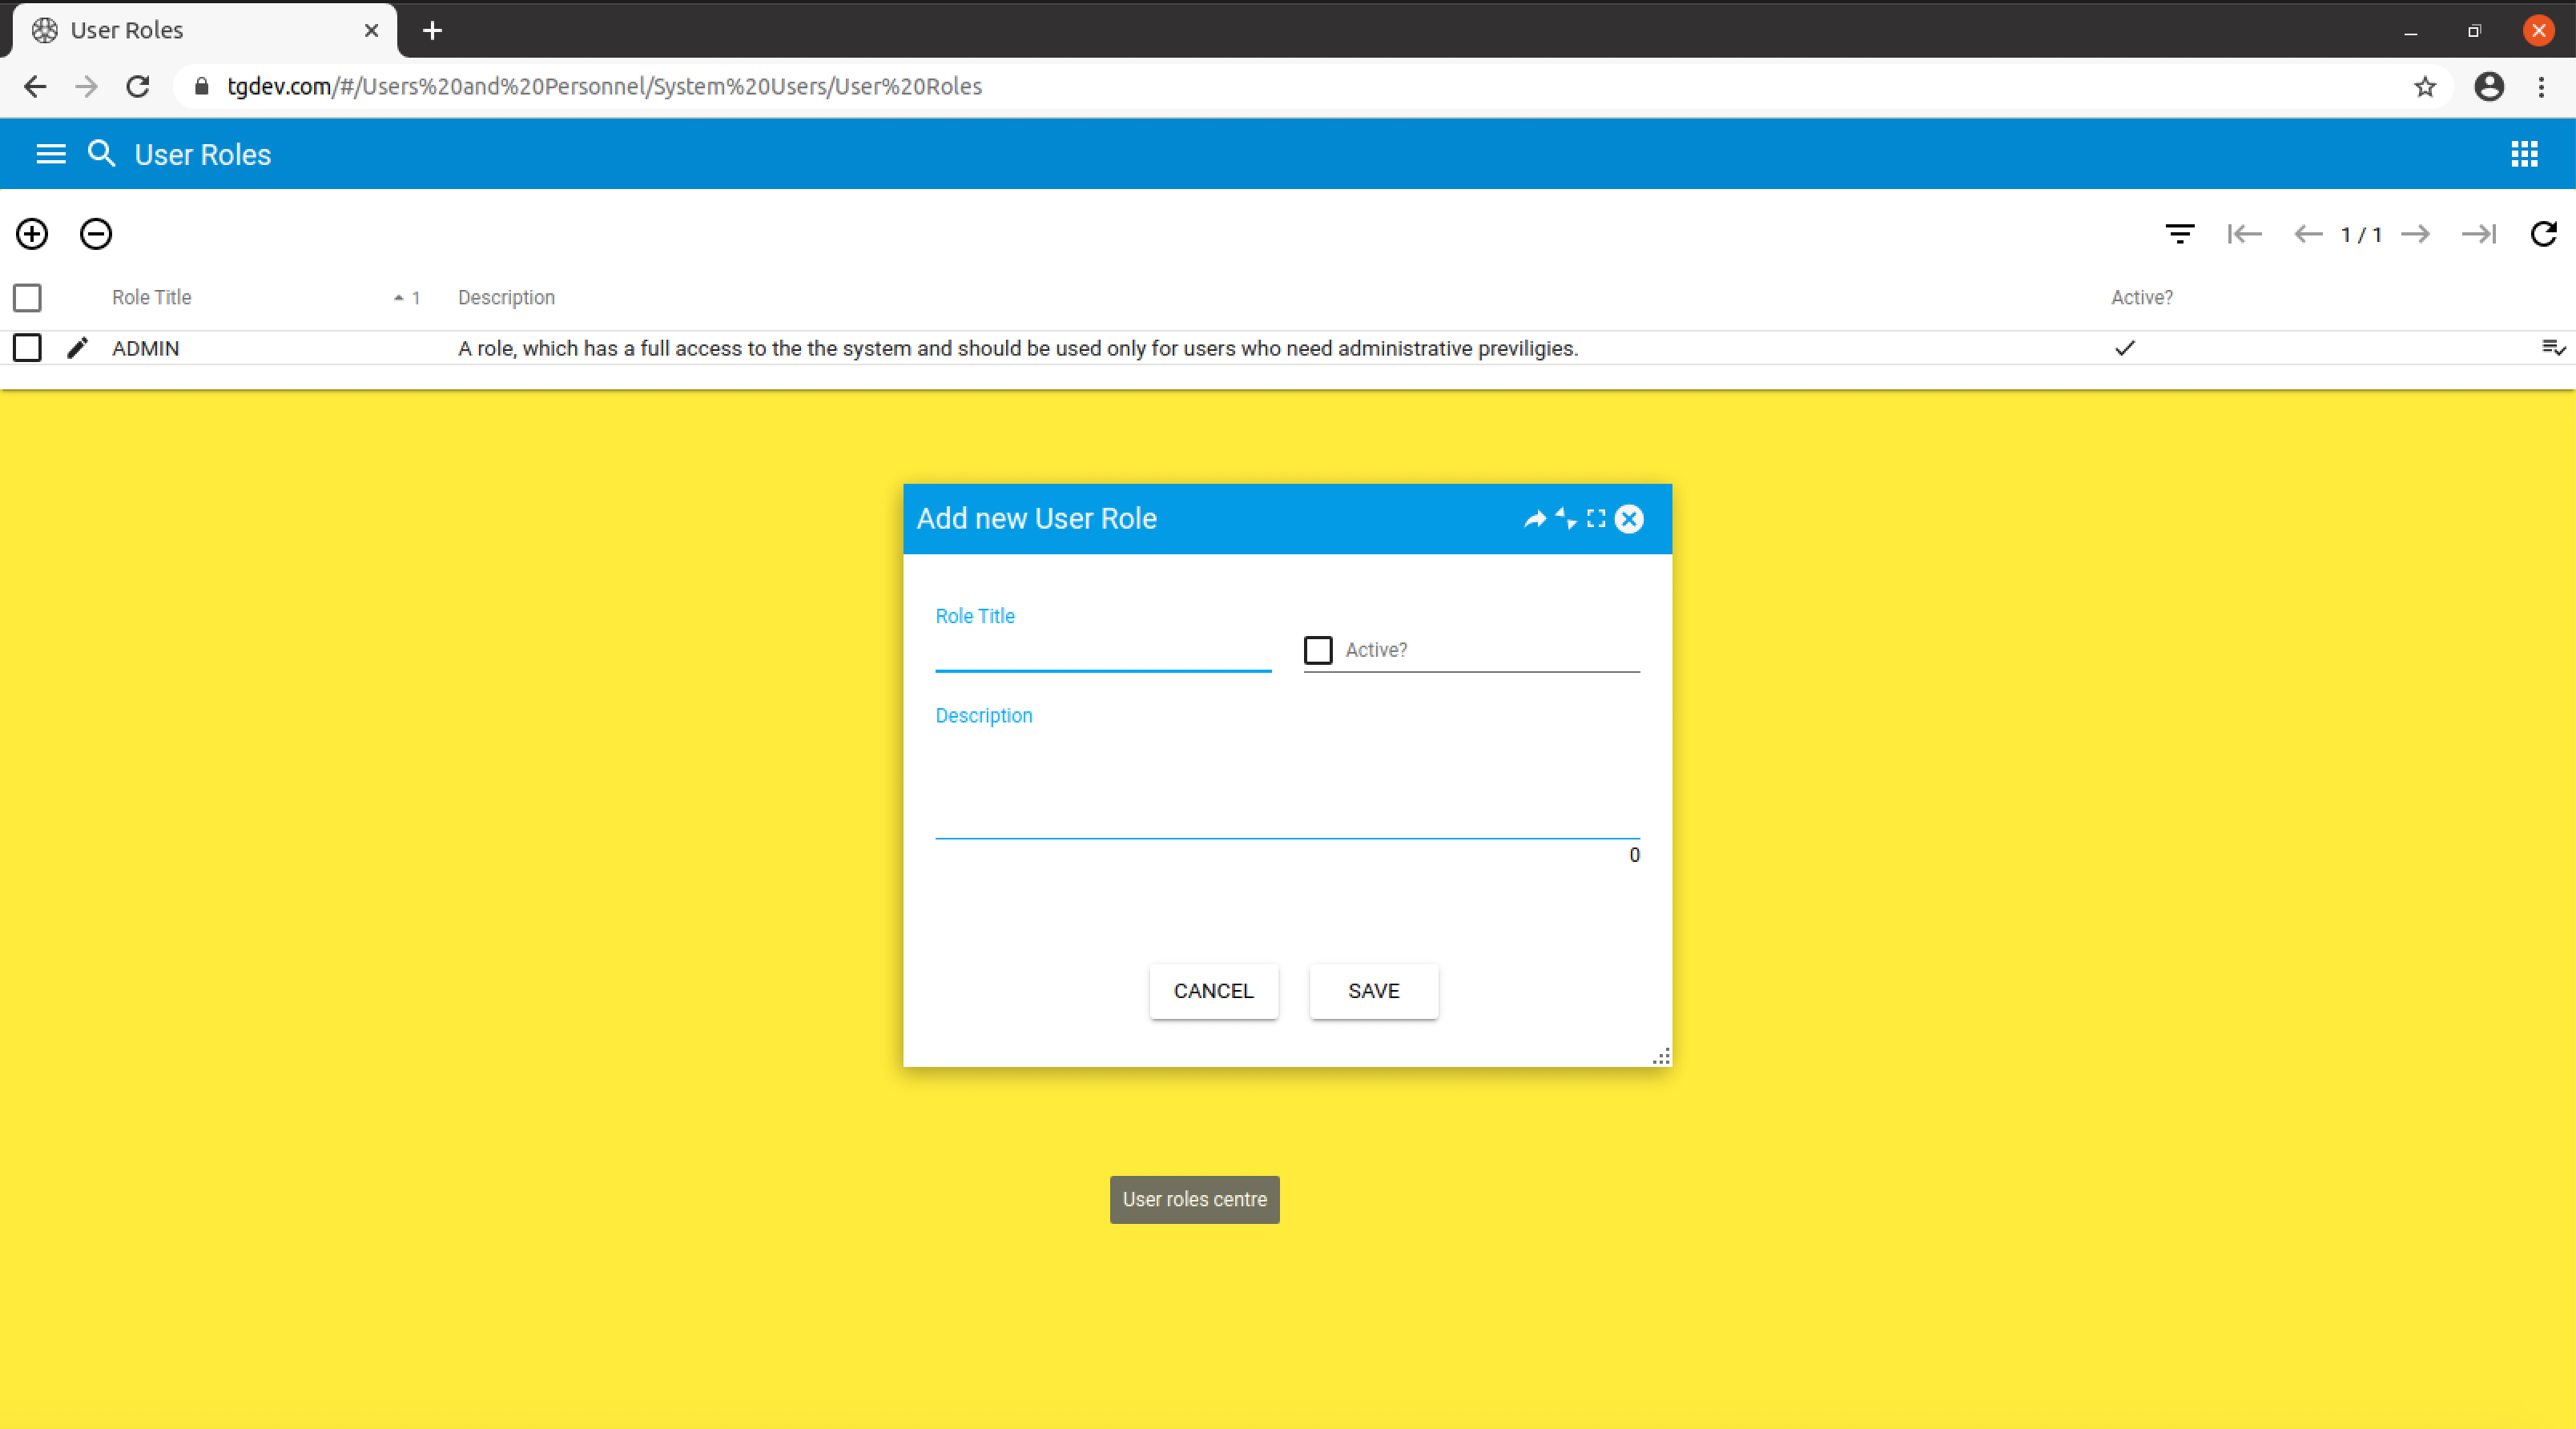
\includegraphics[width=\textwidth]{sections/01-chapter/images/system14.png}

By default we created the ADMIN role. 
The Security Matrix item describes what each role can have access to. 

The tokens do not enable the action by themself. A User has a particular role then it is authorized to make some actions. For example, a user with ADMIN role is authorized to add, edit and delete all the information related to User Entity as well as Person Entity.  

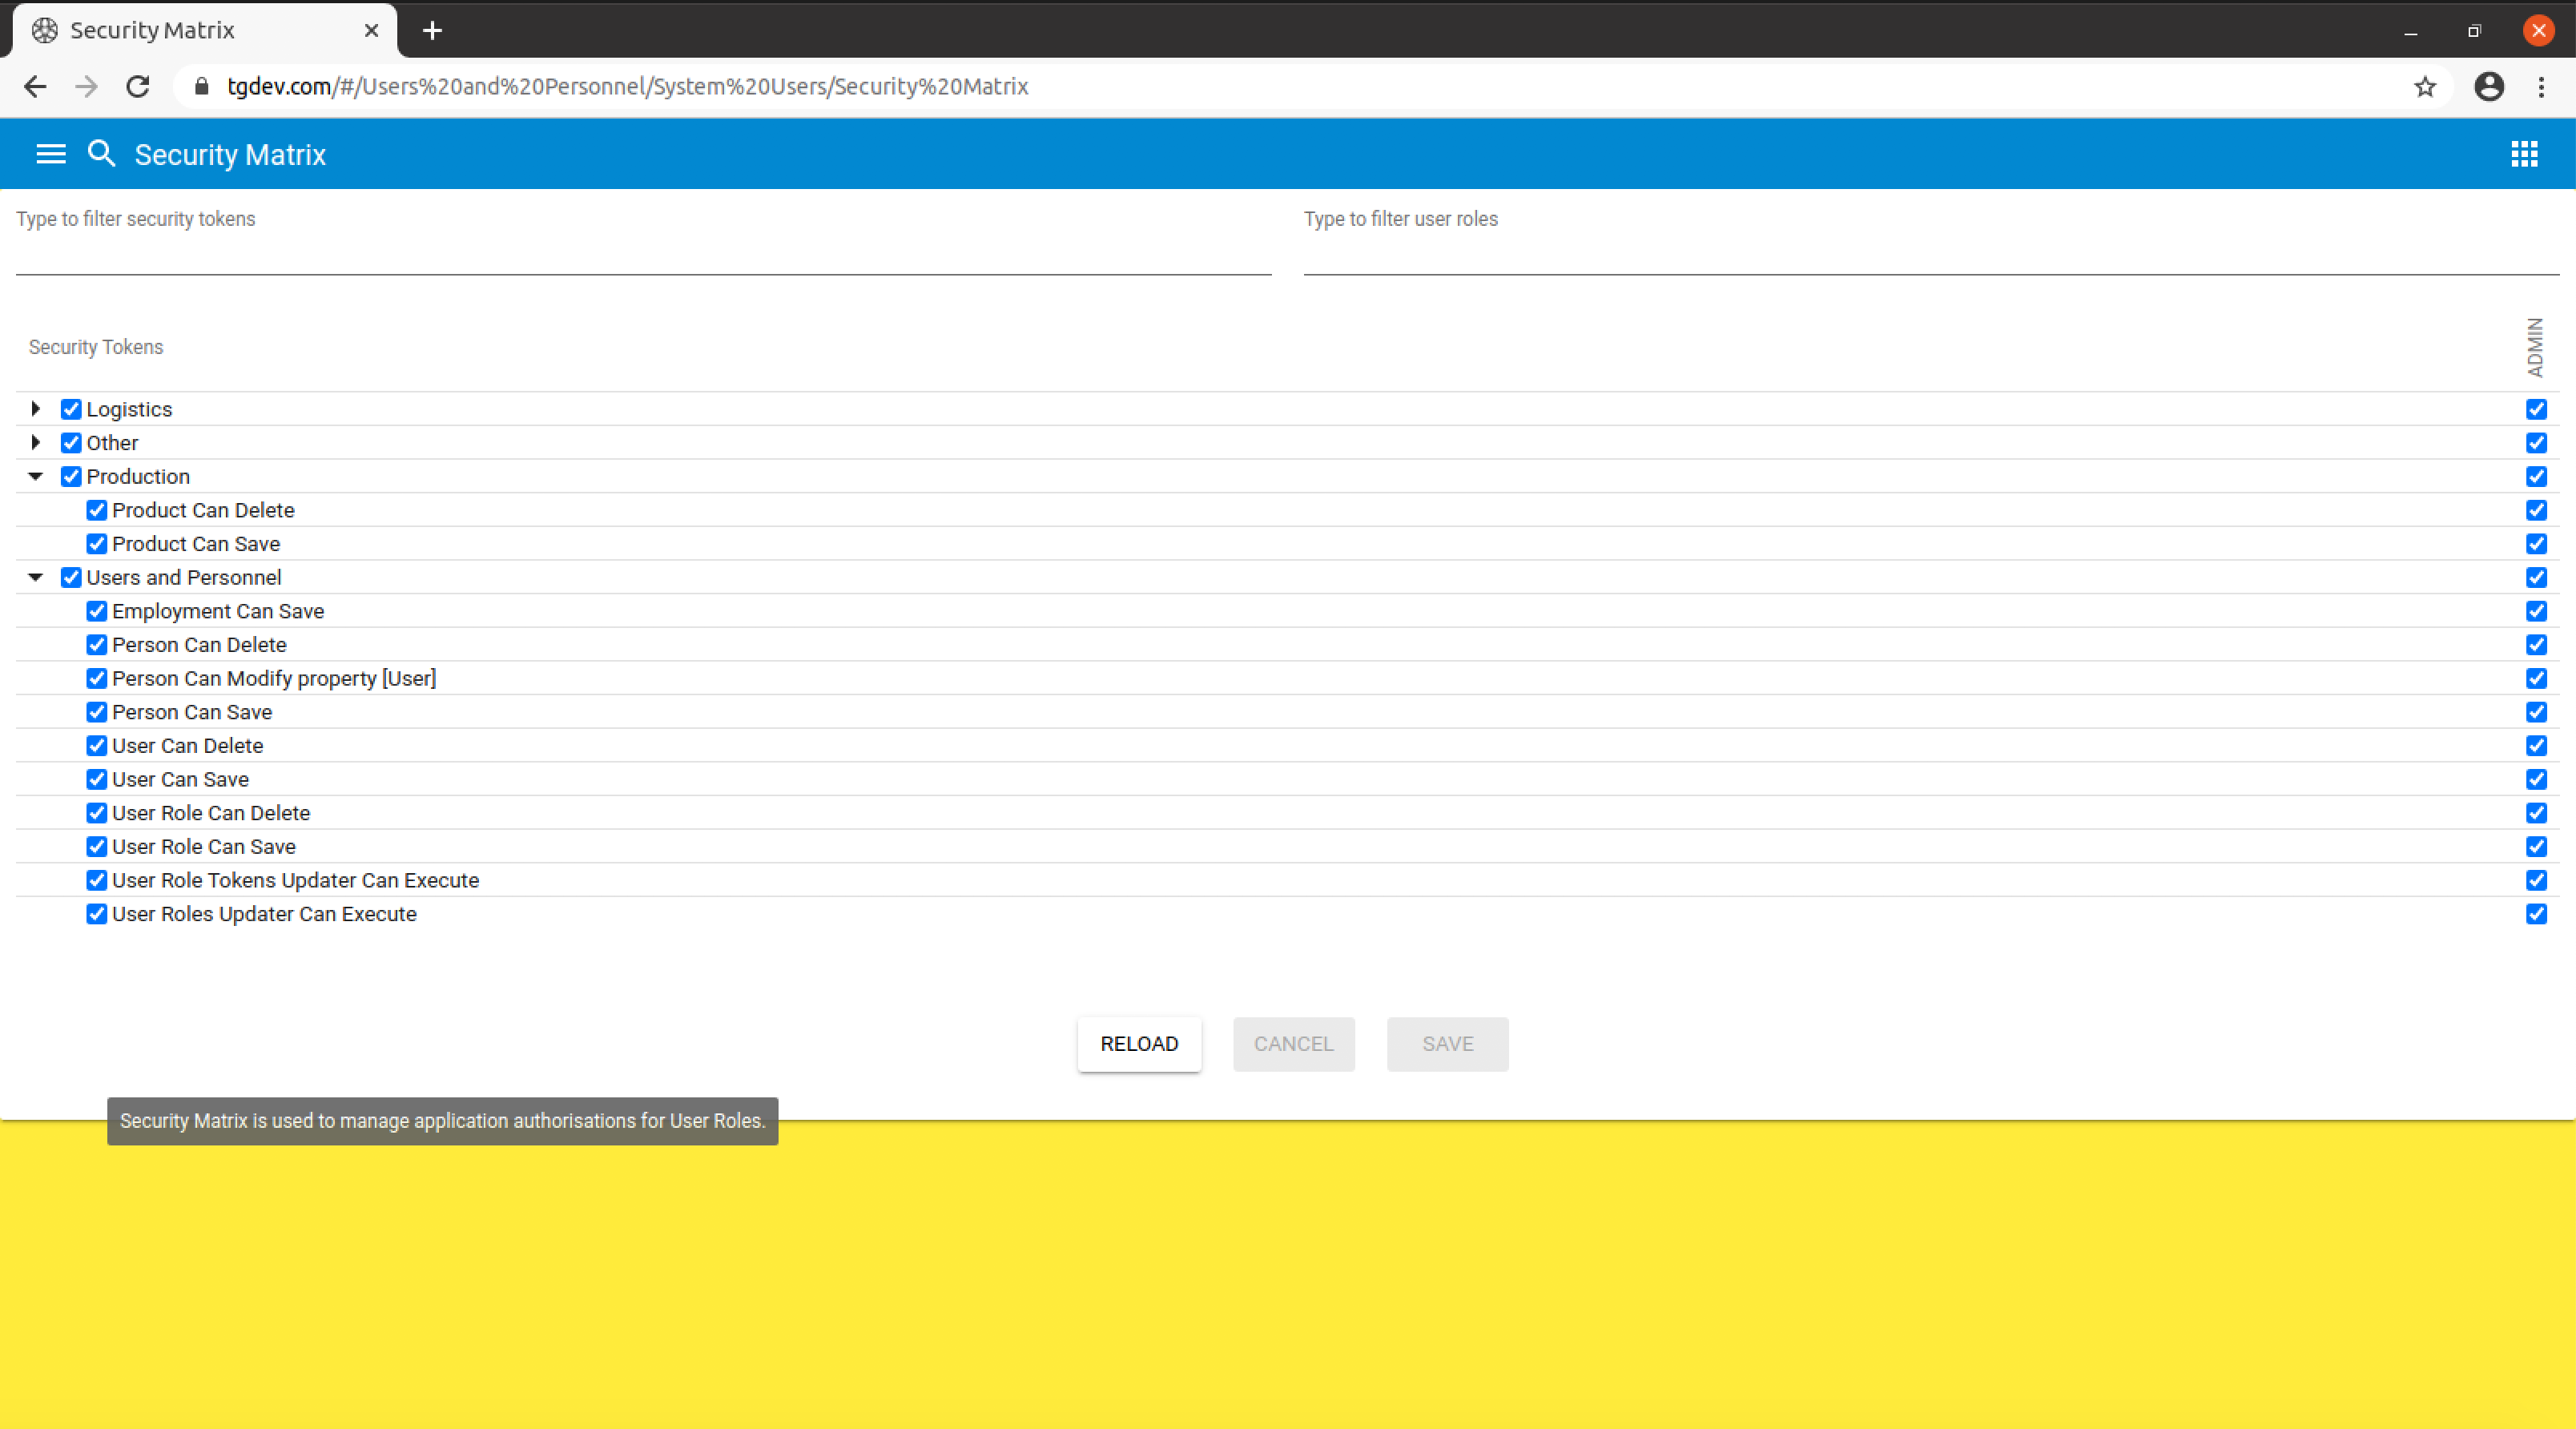
\includegraphics[width=\textwidth]{sections/01-chapter/images/system155.png}

During the assignment of the authorization zones You should be aware that the zones are nested and the outermost will be the one a user will have access to. 

\section{Contact information}
In case of further questions, You can post questions as the separate issue o GitHub: https://github.com/vlad-bilyk/Bakery or write them directly to one of the team members. 

Vlad Bilyk  →  bilyk@ucu.edu.ua

Sofiya Garkot  →  garkot@ucu.edu.ua

Sofiia Tatosh  →  tatosh@ucu.edu.ua

Solomiia Shuptar  →  shuptar@ucu.edu.ua

Nazar Todoshchuk  →  todoshchuk@ucu.edu.ua
